% Latex header for doxygen 1.8.14
\documentclass[twoside]{book}

% Packages required by doxygen
\usepackage{fixltx2e}
\usepackage{calc}
\usepackage{doxygen}
\usepackage[export]{adjustbox} % also loads graphicx
\usepackage{graphicx}
\usepackage[utf8]{inputenc}
\usepackage{makeidx}
\usepackage{multicol}
\usepackage{multirow}
\PassOptionsToPackage{warn}{textcomp}
\usepackage{textcomp}
\usepackage[nointegrals]{wasysym}
\usepackage[table]{xcolor}

\usepackage{float} % for table floating
\usepackage{tabularx}

% Font selection
\usepackage[T1]{fontenc}
\usepackage[scaled=.90]{helvet}
\usepackage{courier}
\usepackage{amssymb}
\usepackage{sectsty}
\renewcommand{\familydefault}{\sfdefault}
\allsectionsfont{%
  \fontseries{bc}\selectfont%
  \color{darkgray}%
}
\renewcommand{\DoxyLabelFont}{%
  \fontseries{bc}\selectfont%
  \color{darkgray}%
}
\newcommand{\+}{\discretionary{\mbox{\scriptsize$\hookleftarrow$}}{}{}}

% Page & text layout
\usepackage{geometry}
\geometry{%
  a4paper,%
  top=2.5cm,%
  bottom=2.5cm,%
  left=2.5cm,%
  right=2.5cm%
}
\tolerance=750
\hfuzz=15pt
\hbadness=750
\setlength{\emergencystretch}{15pt}
\setlength{\parindent}{0cm}
\setlength{\parskip}{3ex plus 2ex minus 2ex}
\makeatletter
\renewcommand{\paragraph}{%
  \@startsection{paragraph}{4}{0ex}{-1.0ex}{1.0ex}{%
    \normalfont\normalsize\bfseries\SS@parafont%
  }%
}
\renewcommand{\subparagraph}{%
  \@startsection{subparagraph}{5}{0ex}{-1.0ex}{1.0ex}{%
    \normalfont\normalsize\bfseries\SS@subparafont%
  }%
}
\makeatother

% Headers & footers
\usepackage{fancyhdr}
\pagestyle{fancyplain}
\fancyhead[LE]{\fancyplain{}{\bfseries\thepage}}
\fancyhead[CE]{\fancyplain{}{}}
\fancyhead[RE]{\fancyplain{}{\bfseries\leftmark}}
\fancyhead[LO]{\fancyplain{}{\bfseries\rightmark}}
\fancyhead[CO]{\fancyplain{}{}}
\fancyhead[RO]{\fancyplain{}{\bfseries\thepage}}
\fancyfoot[LE]{\fancyplain{}{}}
\fancyfoot[CE]{\fancyplain{}{}}
\fancyfoot[RE]{\fancyplain{}{\bfseries\scriptsize Generated by Doxygen }}
\fancyfoot[LO]{\fancyplain{}{\bfseries\scriptsize Generated by Doxygen }}
\fancyfoot[CO]{\fancyplain{}{}}
\fancyfoot[RO]{\fancyplain{}{}}
\renewcommand{\footrulewidth}{0.4pt}
\renewcommand{\chaptermark}[1]{%
  \markboth{#1}{}%
}
\renewcommand{\sectionmark}[1]{%
  \markright{\thesection\ #1}%
}

% Indices & bibliography
\usepackage{natbib}
\usepackage[titles]{tocloft}
\setcounter{tocdepth}{3}
\setcounter{secnumdepth}{5}
\makeindex

% Hyperlinks (required, but should be loaded last)
\usepackage{ifpdf}
\ifpdf
  \usepackage[pdftex,pagebackref=true]{hyperref}
\else
  \usepackage[ps2pdf,pagebackref=true]{hyperref}
\fi
\hypersetup{%
  colorlinks=true,%
  linkcolor=blue,%
  citecolor=blue,%
  unicode%
}

% Custom commands
\newcommand{\clearemptydoublepage}{%
  \newpage{\pagestyle{empty}\cleardoublepage}%
}

\usepackage{caption}
\captionsetup{labelsep=space,justification=centering,font={bf},singlelinecheck=off,skip=4pt,position=top}

%===== C O N T E N T S =====

\begin{document}

% Titlepage & ToC
\hypersetup{pageanchor=false,
             bookmarksnumbered=true,
             pdfencoding=unicode
            }
\pagenumbering{alph}
\begin{titlepage}
\vspace*{7cm}
\begin{center}%
{\Large \textbf{Vehicle Control Unit (VCU) }}\\
\vspace*{1cm}
{\large \textbf{Firmware Specifications}}\\
\end{center}
\end{titlepage}
\clearemptydoublepage
\pagenumbering{roman}

\begin{center}
{\Large \textbf{History}}\\
\vspace*{1cm}
\begin{table}[htbp]
    \centering
    %\begin{tabularx}{\textwidth}{| X | X | X |}
    \begin{tabularx}{\textwidth}{| X | X | X |}
        \hline
		\textbf{Version} & \textbf{Author} & \textbf{Date} \\ \hline
		1.0              & Arella Matteo   & 2018          \\ \hline
	\end{tabularx}
\end{table}
\end{center}

\tableofcontents
\clearemptydoublepage
\pagenumbering{arabic}
\hypersetup{pageanchor=true}

%--- Begin generated contents ---
\chapter{Fast\+Charge\+S\+AE V\+CU firmware}
\label{index}\hypertarget{index}{}Vehicle Control Unit (V\-C\-U) firmware is based upon 4 states\-:
\begin{DoxyItemize}
\item S\-T\-A\-N\-D\-: stato 0, accensione della vettura, si ritorna qui ogni volta che casca l'S\-C
\item H\-V\-O\-N\-: stato 1, alta tensione attiva si accede solo da S\-T\-A\-N\-D tramite A\-I\-Rbutton e S\-C$>$3\-V
\item D\-R\-I\-V\-E\-: stato 2, lo stato di guida sicura, accedibile tramite procedura R\-T\-D ma anche con lo scatto delle plausibilità tramite procedura di rientro 
\end{DoxyItemize}
\chapter{C\+AN Networks}
\label{_c_a_n}
\Hypertarget{_c_a_n}
Two C\+AN networks have been designed to be inserted into the vehicle\+: a first C\+AN network between the V\+CU and the inverter (C\+AN funzionale) and a second C\+AN network between the V\+CU, T\+CU and S\+C\+Us (C\+AN servizi).

Each node connected to C\+AN network has an unique ID internally to that network, according to this table\+: \tabulinesep=1mm
\begin{longtabu} spread 0pt [c]{*{3}{|X[-1]}|}
\hline
\rowcolor{\tableheadbgcolor}\textbf{ C\+AN N\+E\+T\+W\+O\+RK  }&\textbf{ N\+O\+DE  }&\textbf{ N\+O\+D\+E-\/\+ID   }\\\cline{1-3}
\endfirsthead
\hline
\endfoot
\hline
\rowcolor{\tableheadbgcolor}\textbf{ C\+AN N\+E\+T\+W\+O\+RK  }&\textbf{ N\+O\+DE  }&\textbf{ N\+O\+D\+E-\/\+ID   }\\\cline{1-3}
\endhead
\multirow{2}{\linewidth}{F\+U\+N\+Z\+I\+O\+N\+A\+LE  }&I\+N\+V\+E\+R\+T\+ER  &1   \\\cline{2-3}
&V\+CU  &2   \\\cline{1-3}
\multirow{3}{\linewidth}{S\+E\+R\+V\+I\+ZI  }&Frontal\+S\+CU  &1   \\\cline{2-3}
&V\+CU  &2   \\\cline{2-3}
&T\+CU  &4   \\\cline{1-3}
\end{longtabu}



\begin{DoxyItemize}
\item \mbox{\hyperlink{CAN_funzionale_page}{C\+AN funzionale}}
\item \mbox{\hyperlink{CAN_servizi_page}{C\+AN servizi}} 
\end{DoxyItemize}\hypertarget{CAN_funzionale_page}{}\section{C\+AN Funzionale}\label{CAN_funzionale_page}
C\+AN funzionale network arises from the need to have an high reliable and robust communication between V\+CU and inverter.

\subsection*{V\+CU master on power up sequence}


\begin{DoxyEnumerate}
\item {\bfseries wait for B\+O\+O\+T-\/\+UP message from inverter} ~\newline
 \tabulinesep=1mm
\begin{longtabu} spread 0pt [c]{*{2}{|X[-1]}|}
\hline
\rowcolor{\tableheadbgcolor}\textbf{ C\+O\+B-\/\+ID (11bits)  }&\textbf{ data byte 0   }\\\cline{1-2}
\endfirsthead
\hline
\endfoot
\hline
\rowcolor{\tableheadbgcolor}\textbf{ C\+O\+B-\/\+ID (11bits)  }&\textbf{ data byte 0   }\\\cline{1-2}
\endhead
0x700 + N\+O\+D\+E-\/\+ID  &0x00   \\\cline{1-2}
\end{longtabu}



\item {\bfseries check V\+E\+N\+D\+O\+R-\/\+ID} (V\+CU read object 0x1018) ~\newline
 {\itshape V\+CU send cliend S\+DO} \tabulinesep=1mm
\begin{longtabu} spread 0pt [c]{*{5}{|X[-1]}|}
\hline
\rowcolor{\tableheadbgcolor}\textbf{ C\+O\+B-\/\+ID (11bits)  }&\textbf{ Command byte  }&\textbf{ Obj. Index (2 byte)  }&\textbf{ Obj. sub-\/index (byte)  }&\textbf{ Data (4bytes)   }\\\cline{1-5}
\endfirsthead
\hline
\endfoot
\hline
\rowcolor{\tableheadbgcolor}\textbf{ C\+O\+B-\/\+ID (11bits)  }&\textbf{ Command byte  }&\textbf{ Obj. Index (2 byte)  }&\textbf{ Obj. sub-\/index (byte)  }&\textbf{ Data (4bytes)   }\\\cline{1-5}
\endhead
0x600 + N\+O\+D\+E-\/\+ID  &0x40  &0x1810  &0x01  &0   \\\cline{1-5}
\end{longtabu}
~\newline
 {\itshape V\+CU receive server S\+DO (from inverter)} \tabulinesep=1mm
\begin{longtabu} spread 0pt [c]{*{5}{|X[-1]}|}
\hline
\rowcolor{\tableheadbgcolor}\textbf{ C\+O\+B-\/\+ID (11bits)  }&\textbf{ Command byte  }&\textbf{ Obj. Index (2 byte)  }&\textbf{ Obj. sub-\/index (byte)  }&\textbf{ Data (4bytes)   }\\\cline{1-5}
\endfirsthead
\hline
\endfoot
\hline
\rowcolor{\tableheadbgcolor}\textbf{ C\+O\+B-\/\+ID (11bits)  }&\textbf{ Command byte  }&\textbf{ Obj. Index (2 byte)  }&\textbf{ Obj. sub-\/index (byte)  }&\textbf{ Data (4bytes)   }\\\cline{1-5}
\endhead
0x580 + N\+O\+D\+E-\/\+ID  &0x43  &0x1810  &0x01  &0x19030000   \\\cline{1-5}
\end{longtabu}



\item {\bfseries send N\+MT \textquotesingle{}go Operational\textquotesingle{}} (broadcast) \tabulinesep=1mm
\begin{longtabu} spread 0pt [c]{*{3}{|X[-1]}|}
\hline
\rowcolor{\tableheadbgcolor}\textbf{ C\+O\+B-\/\+ID (11bits)  }&\textbf{ data byte 0  }&\textbf{ data byte 1   }\\\cline{1-3}
\endfirsthead
\hline
\endfoot
\hline
\rowcolor{\tableheadbgcolor}\textbf{ C\+O\+B-\/\+ID (11bits)  }&\textbf{ data byte 0  }&\textbf{ data byte 1   }\\\cline{1-3}
\endhead
0x000  &0x01  &0x00   \\\cline{1-3}
\end{longtabu}



\item {\bfseries send P\+DO to enable P\+WM} ~\newline
 \tabulinesep=1mm
\begin{longtabu} spread 0pt [c]{*{2}{|X[-1]}|}
\hline
\rowcolor{\tableheadbgcolor}\textbf{ C\+O\+B-\/\+ID (11bits)  }&\textbf{ Data (R\+P\+D\+O1)   }\\\cline{1-2}
\endfirsthead
\hline
\endfoot
\hline
\rowcolor{\tableheadbgcolor}\textbf{ C\+O\+B-\/\+ID (11bits)  }&\textbf{ Data (R\+P\+D\+O1)   }\\\cline{1-2}
\endhead
0x200 + N\+O\+D\+E-\/\+ID  &06 00 xx xx xx xx xx xx   \\\cline{1-2}
\end{longtabu}
~\newline
 \tabulinesep=1mm
\begin{longtabu} spread 0pt [c]{*{2}{|X[-1]}|}
\hline
\rowcolor{\tableheadbgcolor}\textbf{ C\+O\+B-\/\+ID (11bits)  }&\textbf{ Data (R\+P\+D\+O1)   }\\\cline{1-2}
\endfirsthead
\hline
\endfoot
\hline
\rowcolor{\tableheadbgcolor}\textbf{ C\+O\+B-\/\+ID (11bits)  }&\textbf{ Data (R\+P\+D\+O1)   }\\\cline{1-2}
\endhead
0x200 + N\+O\+D\+E-\/\+ID  &07 00 xx xx xx xx xx xx   \\\cline{1-2}
\end{longtabu}
~\newline
 \tabulinesep=1mm
\begin{longtabu} spread 0pt [c]{*{2}{|X[-1]}|}
\hline
\rowcolor{\tableheadbgcolor}\textbf{ C\+O\+B-\/\+ID (11bits)  }&\textbf{ Data (R\+P\+D\+O1)   }\\\cline{1-2}
\endfirsthead
\hline
\endfoot
\hline
\rowcolor{\tableheadbgcolor}\textbf{ C\+O\+B-\/\+ID (11bits)  }&\textbf{ Data (R\+P\+D\+O1)   }\\\cline{1-2}
\endhead
0x200 + N\+O\+D\+E-\/\+ID  &0F 00 xx xx xx xx xx xx   \\\cline{1-2}
\end{longtabu}



\item {\bfseries periodically send S\+Y\+NC message} ~\newline
 {\itshape V\+CU broadcast S\+Y\+NC} \tabulinesep=1mm
\begin{longtabu} spread 0pt [c]{*{2}{|X[-1]}|}
\hline
\rowcolor{\tableheadbgcolor}\textbf{ C\+O\+B-\/\+ID (11bits)  }&\textbf{ Data byte 0   }\\\cline{1-2}
\endfirsthead
\hline
\endfoot
\hline
\rowcolor{\tableheadbgcolor}\textbf{ C\+O\+B-\/\+ID (11bits)  }&\textbf{ Data byte 0   }\\\cline{1-2}
\endhead
0x80 + N\+O\+D\+E-\/\+ID  &0x00   \\\cline{1-2}
\end{longtabu}

\end{DoxyEnumerate}\hypertarget{CAN_servizi_page}{}\section{C\+AN Servizi}\label{CAN_servizi_page}
C\+AN servizi network arises from the need to digitize all those signals necessary for the operation of the car. V\+CU master node is interested to receive pedals position percentage values, A\+P\+PS and brake plausibility from frontal S\+CU, and torque request limiter from T\+CU.

A C\+A\+Nbus communication protocol has been developed based on the C\+A\+Nopen specifications (CiA 301). Each slave node can be represented by a finite state machine with the following states\+: Initialisation, Pre-\/operational, Operational, Stopped. During power-\/up each node is in the Initialization phase. At the end of this phase, it attempts to send a boot-\/up message. As soon as it has been successfully sent, it is placed in the Pre-\/operational state. Using an N\+MT master message, the V\+CU can passes the various slave nodes between the different Pre-\/operational, Operational and Stopped states.

\subsection*{V\+CU master on power up sequence}


\begin{DoxyEnumerate}
\item {\bfseries wait for B\+O\+O\+T-\/\+UP message from slave nodes} (from frontal S\+CU and T\+CU) \tabulinesep=1mm
\begin{longtabu} spread 0pt [c]{*{2}{|X[-1]}|}
\hline
\rowcolor{\tableheadbgcolor}\textbf{ C\+O\+B-\/\+ID (11bits)  }&\textbf{ data byte 0   }\\\cline{1-2}
\endfirsthead
\hline
\endfoot
\hline
\rowcolor{\tableheadbgcolor}\textbf{ C\+O\+B-\/\+ID (11bits)  }&\textbf{ data byte 0   }\\\cline{1-2}
\endhead
0x700 + N\+O\+D\+E-\/\+ID  &0x00   \\\cline{1-2}
\end{longtabu}

\item {\bfseries send N\+MT \textquotesingle{}go Operational\textquotesingle{}} (broadcast) \tabulinesep=1mm
\begin{longtabu} spread 0pt [c]{*{3}{|X[-1]}|}
\hline
\rowcolor{\tableheadbgcolor}\textbf{ C\+O\+B-\/\+ID (11bits)  }&\textbf{ data byte 0  }&\textbf{ data byte 1   }\\\cline{1-3}
\endfirsthead
\hline
\endfoot
\hline
\rowcolor{\tableheadbgcolor}\textbf{ C\+O\+B-\/\+ID (11bits)  }&\textbf{ data byte 0  }&\textbf{ data byte 1   }\\\cline{1-3}
\endhead
0x000  &0x01  &0x00   \\\cline{1-3}
\end{longtabu}

\end{DoxyEnumerate}

\subsection*{Fault Tolerance}

If failure of C\+AN servizi network occurs, redundancy has been introduced in the acquisition of pedals\+: if P\+DO with the pedal data are not received within a certain timeout then C\+AN servizi network is considered non-\/functional and pedal sensors are acquired directly via analog signals from the V\+CU. 
\chapter{Board model}
\label{_model_page}
\Hypertarget{_model_page}
V\+CU is based on an Atmel S\+A\+M3\+X8E board with an A\+RM Cortex-\/\+M3 microprocessor.

IO signals managed from V\+CU are\+:
\begin{DoxyItemize}
\item A\+N\+A\+L\+OG
\begin{DoxyEnumerate}
\item First A\+P\+PS
\item Second A\+P\+PS
\item Brake pedal position sensor
\item SC voltage
\end{DoxyEnumerate}
\item D\+I\+G\+I\+T\+AL
\begin{DoxyEnumerate}
\item A\+I\+R+
\item A\+I\+R-\/
\item Precharge
\item R\+T\+DS buzzer
\item A\+IR button
\item R\+TD button
\end{DoxyEnumerate}
\end{DoxyItemize}

In case of \mbox{\hyperlink{CAN_servizi_page}{C\+AN Servizi}} failure both A\+P\+PS and brake pedal position sensor are acquired by analog signals for fault tolerance. 
\chapter{Ready To Drive Sound (R\+T\+DS)}
\label{_r_t_d_s}
\Hypertarget{_r_t_d_s}
The vehicle must make a characteristic sound, continuously for at least one second and a maximum of three seconds when it enters ready-\/to-\/drive mode. According \mbox{\hyperlink{_f_s_m_page}{Finite State Machine (F\+SM)}}, R\+T\+DS is triggered with transition from \mbox{\hyperlink{_f_s_m_page_HVON}{H\+V\+ON}} state to \mbox{\hyperlink{_f_s_m_page_DRIVE}{D\+R\+I\+VE}} state. 
\chapter{Finite State Machine (F\+SM)}
\label{_f_s_m_page}
\Hypertarget{_f_s_m_page}
V\+CU firmware is based upon 4 states\+:
\begin{DoxyItemize}
\item \label{_f_s_m_page_STAND}%
\Hypertarget{_f_s_m_page_STAND}%
\char`\"{}\+S\+T\+A\+N\+D\char`\"{}\+: ignition of the car, you return here every time SC is undervoltage
\item \label{_f_s_m_page_HVON}%
\Hypertarget{_f_s_m_page_HVON}%
\char`\"{}\+H\+V O\+N\char`\"{}\+: active high voltage is only accessed from S\+T\+A\+ND via A\+I\+Rbutton and SC voltage $>$ 3V
\item \label{_f_s_m_page_DRIVE}%
\Hypertarget{_f_s_m_page_DRIVE}%
\char`\"{}\+D\+R\+I\+V\+E\char`\"{}\+: the safe driving status, accessible by R\+TD procedure but also with pedals implausibility through the return procedure
\item \label{_f_s_m_page_NOTDRIVE}%
\Hypertarget{_f_s_m_page_NOTDRIVE}%
\char`\"{}\+N\+O\+T D\+R\+I\+V\+E\char`\"{}\+: error with pedals, the sensors of the pedals are disconnected or out range. Torque request and braking request are disabled; you enter only by pedals implausibility or absence of the brake.
\end{DoxyItemize}

 
\begin{DoxyImage}
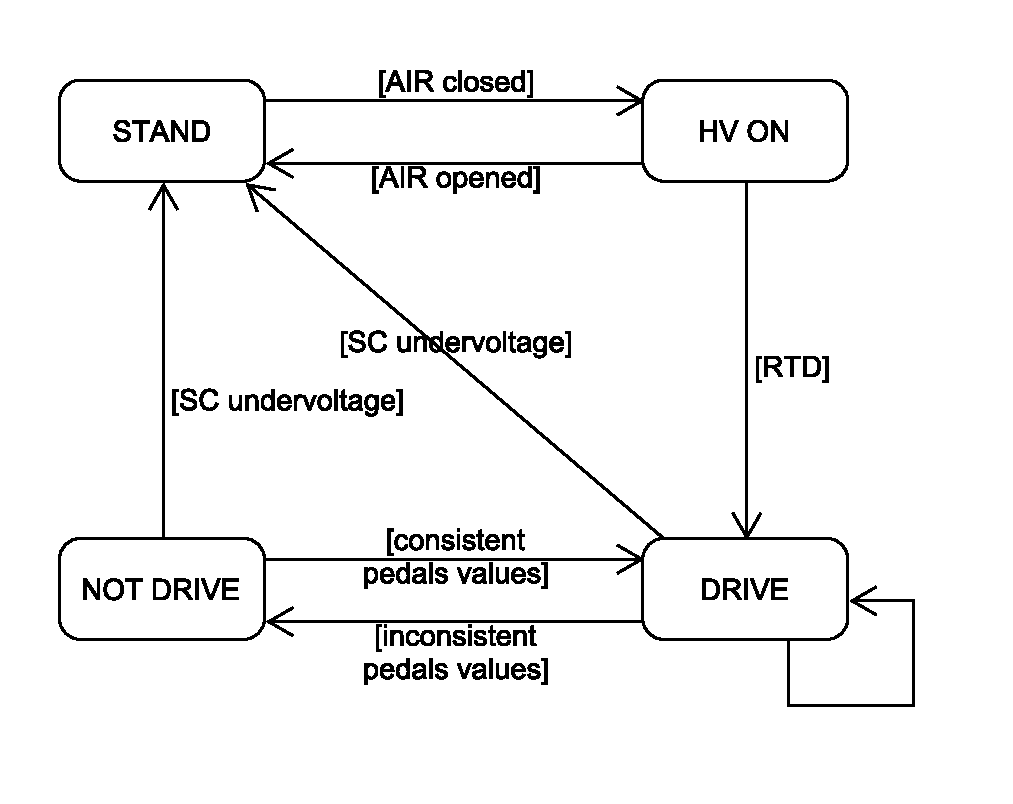
\includegraphics[width=10cm]{fsm_diagram}
\doxyfigcaption{F\+SM diagram}
\end{DoxyImage}
 
\chapter{Module Index}
\section{Modules}
Here is a list of all modules\-:\begin{DoxyCompactList}
\item \contentsline{section}{C\-A\-N\-\_\-module\-\_\-group}{\pageref{group___c_a_n__module__group}}{}
\begin{DoxyCompactList}
\item \contentsline{section}{C\-A\-N\-\_\-funzionale\-\_\-group}{\pageref{group___c_a_n__funzionale__group}}{}
\item \contentsline{section}{C\-A\-N\-\_\-servizi\-\_\-group}{\pageref{group___c_a_n__servizi__group}}{}
\end{DoxyCompactList}
\item \contentsline{section}{Board\-\_\-model\-\_\-group}{\pageref{group___board__model__group}}{}
\item \contentsline{section}{R\-T\-D\-S\-\_\-group}{\pageref{group___r_t_d_s__group}}{}
\end{DoxyCompactList}

\chapter{File Index}
\section{File List}
Here is a list of all documented files with brief descriptions\+:\begin{DoxyCompactList}
\item\contentsline{section}{{\bfseries board\+\_\+pinout.\+h} }{\pageref{board__pinout_8h}}{}
\item\contentsline{section}{\mbox{\hyperlink{can__funzionale_8cpp}{can\+\_\+funzionale.\+cpp}} \\*C\+AN funzionale module implementation }{\pageref{can__funzionale_8cpp}}{}
\item\contentsline{section}{\mbox{\hyperlink{can__funzionale_8h}{can\+\_\+funzionale.\+h}} \\*C\+AN funzionale module header }{\pageref{can__funzionale_8h}}{}
\item\contentsline{section}{\mbox{\hyperlink{_c_a_n___i_d_8h}{C\+A\+N\+\_\+\+I\+D.\+h}} \\*C\+AN nodes ID definitions module }{\pageref{_c_a_n___i_d_8h}}{}
\item\contentsline{section}{\mbox{\hyperlink{can__servizi_8cpp}{can\+\_\+servizi.\+cpp}} \\*C\+AN servizi module implementation }{\pageref{can__servizi_8cpp}}{}
\item\contentsline{section}{\mbox{\hyperlink{can__servizi_8h}{can\+\_\+servizi.\+h}} \\*C\+AN servizi module header }{\pageref{can__servizi_8h}}{}
\item\contentsline{section}{\mbox{\hyperlink{_c_o__can_8cpp}{C\+O\+\_\+can.\+cpp}} \\*C\+AN setup module implementation }{\pageref{_c_o__can_8cpp}}{}
\item\contentsline{section}{\mbox{\hyperlink{_c_o__can_8h}{C\+O\+\_\+can.\+h}} \\*C\+AN setup header module }{\pageref{_c_o__can_8h}}{}
\item\contentsline{section}{\mbox{\hyperlink{common_8h}{common.\+h}} \\*Common macro definitions module }{\pageref{common_8h}}{}
\item\contentsline{section}{{\bfseries def.\+h} }{\pageref{def_8h}}{}
\item\contentsline{section}{{\bfseries filter.\+cpp} }{\pageref{filter_8cpp}}{}
\item\contentsline{section}{{\bfseries filter.\+h} }{\pageref{filter_8h}}{}
\item\contentsline{section}{\mbox{\hyperlink{model_8cpp}{model.\+cpp}} \\*Board model implementation file }{\pageref{model_8cpp}}{}
\item\contentsline{section}{\mbox{\hyperlink{model_8h}{model.\+h}} \\*Board model header file }{\pageref{model_8h}}{}
\item\contentsline{section}{{\bfseries rtds.\+cpp} }{\pageref{rtds_8cpp}}{}
\item\contentsline{section}{{\bfseries rtds.\+h} }{\pageref{rtds_8h}}{}
\item\contentsline{section}{{\bfseries states.\+cpp} }{\pageref{states_8cpp}}{}
\item\contentsline{section}{{\bfseries states.\+h} }{\pageref{states_8h}}{}
\item\contentsline{section}{\mbox{\hyperlink{_v_c_u_8ino}{V\+C\+U.\+ino}} \\*Main module file }{\pageref{_v_c_u_8ino}}{}
\end{DoxyCompactList}

\chapter{Module Documentation}
\hypertarget{group___c_a_n__module__group}{\section{C\-A\-N\-\_\-module\-\_\-group}
\label{group___c_a_n__module__group}\index{C\-A\-N\-\_\-module\-\_\-group@{C\-A\-N\-\_\-module\-\_\-group}}
}
\subsection*{Modules}
\begin{DoxyCompactItemize}
\item 
\hyperlink{group___c_a_n__funzionale__group}{C\-A\-N\-\_\-funzionale\-\_\-group}
\item 
\hyperlink{group___c_a_n__servizi__group}{C\-A\-N\-\_\-servizi\-\_\-group}
\end{DoxyCompactItemize}
\subsection*{Macros}
\begin{DoxyCompactItemize}
\item 
\hypertarget{group___c_a_n__module__group_ga5703fd8de5ab8d0dcedb561f2178829e}{\#define \hyperlink{group___c_a_n__module__group_ga5703fd8de5ab8d0dcedb561f2178829e}{V\-C\-U\-\_\-\-N\-O\-D\-E\-\_\-\-I\-D}~2}\label{group___c_a_n__module__group_ga5703fd8de5ab8d0dcedb561f2178829e}

\begin{DoxyCompactList}\small\item\em V\-C\-U Node I\-D. \end{DoxyCompactList}\end{DoxyCompactItemize}
\subsection*{Functions}
\begin{DoxyCompactItemize}
\item 
bool \hyperlink{group___c_a_n__module__group_ga36b6b5924eb84ef2e4c2bd548b28436f}{can\-\_\-init} ()
\begin{DoxyCompactList}\small\item\em This function initializes both C\-A\-N funzionale and C\-A\-N servizi networks. \end{DoxyCompactList}\end{DoxyCompactItemize}


\subsection{Detailed Description}


\subsection{Function Documentation}
\hypertarget{group___c_a_n__module__group_ga36b6b5924eb84ef2e4c2bd548b28436f}{\index{C\-A\-N\-\_\-module\-\_\-group@{C\-A\-N\-\_\-module\-\_\-group}!can\-\_\-init@{can\-\_\-init}}
\index{can\-\_\-init@{can\-\_\-init}!CAN_module_group@{C\-A\-N\-\_\-module\-\_\-group}}
\subsubsection[{can\-\_\-init}]{\setlength{\rightskip}{0pt plus 5cm}bool can\-\_\-init (
\begin{DoxyParamCaption}
{}
\end{DoxyParamCaption}
)}}\label{group___c_a_n__module__group_ga36b6b5924eb84ef2e4c2bd548b28436f}


This function initializes both C\-A\-N funzionale and C\-A\-N servizi networks. 

\begin{DoxyAuthor}{Author}
Arella Matteo \par
 (mail\-: \href{mailto:arella.1646983@studenti.uniroma1.it}{\tt arella.\-1646983@studenti.\-uniroma1.\-it}) 
\end{DoxyAuthor}

\begin{DoxyRetVals}{Return values}
{\em true} & C\-A\-N networks initialized successfully \\
\hline
{\em false} & C\-A\-N networks initialization failed \\
\hline
\end{DoxyRetVals}


Definition at line 26 of file C\-O\-\_\-can.\-cpp.


\hypertarget{group___c_a_n__funzionale__group}{}\section{C\+AN funzionale}
\label{group___c_a_n__funzionale__group}\index{C\+A\+N funzionale@{C\+A\+N funzionale}}
Collaboration diagram for C\+AN funzionale\+:\nopagebreak
\begin{figure}[H]
\begin{center}
\leavevmode
\includegraphics[width=270pt]{group___c_a_n__funzionale__group}
\end{center}
\end{figure}
\subsection*{Macros}
\begin{DoxyCompactItemize}
\item 
\mbox{\Hypertarget{group___c_a_n__funzionale__group_ga59ea82aec4abe07072cbdad555a8c1b9}\label{group___c_a_n__funzionale__group_ga59ea82aec4abe07072cbdad555a8c1b9}} 
\#define \mbox{\hyperlink{group___c_a_n__funzionale__group_ga59ea82aec4abe07072cbdad555a8c1b9}{I\+N\+V\+E\+R\+T\+E\+R\+\_\+\+N\+O\+D\+E\+\_\+\+ID}}~1
\begin{DoxyCompactList}\small\item\em Inverter Node ID. \end{DoxyCompactList}\end{DoxyCompactItemize}
\subsection*{Functions}
\begin{DoxyCompactItemize}
\item 
volatile bool \mbox{\hyperlink{group___c_a_n__funzionale__group_gaf1acdfa5537f47656edd6ffa3e7c24bd}{can\+\_\+funzionale\+\_\+initialized}} ()
\begin{DoxyCompactList}\small\item\em This function returns C\+AN funzionale initialization status. \end{DoxyCompactList}\item 
void \mbox{\hyperlink{group___c_a_n__funzionale__group_gac93bbbf1b84f1bc82b26d54d7f898172}{can\+\_\+funzionale\+\_\+send\+\_\+sync}} ()
\begin{DoxyCompactList}\small\item\em This function sends a periodic C\+A\+N\+Open sync message to inverter slave node. \end{DoxyCompactList}\item 
void \mbox{\hyperlink{group___c_a_n__funzionale__group_gaf4990e00c0c4a9f9eeb9cb5bdaecfa94}{C\+A\+N\+\_\+\+F\+U\+N\+Z\+\_\+\+B\+O\+O\+T\+U\+P\+\_\+\+CB}} (C\+A\+N\+\_\+\+F\+R\+A\+ME $\ast$frame)
\begin{DoxyCompactList}\small\item\em This function manage boot-\/up message sent over C\+AN funzionale network by inverter slave node. Upon boot-\/up message reception the V\+CU send a S\+DO client request for check inverter vendor ID; then inverter is considered online over C\+AN funzionale network. \end{DoxyCompactList}\item 
void \mbox{\hyperlink{group___c_a_n__funzionale__group_ga81bbc4c65d579febfbcae399f0ecbffc}{C\+A\+N\+\_\+\+F\+U\+N\+Z\+\_\+\+V\+E\+N\+D\+O\+R\+\_\+\+I\+D\+\_\+\+CB}} (C\+A\+N\+\_\+\+F\+R\+A\+ME $\ast$frame)
\begin{DoxyCompactList}\small\item\em This function manage S\+DO server response with inverter Vendor ID. V\+CU sends N\+MT operational and P\+D\+Os to enable P\+WM; then inverter is considered correctly configured and a timer is started for sending periodic sync messages. \end{DoxyCompactList}\item 
void \mbox{\hyperlink{group___c_a_n__funzionale__group_ga1fcfa8e31cfbfe2461328c345b5b8e19}{C\+A\+N\+\_\+\+F\+U\+N\+Z\+\_\+\+G\+E\+N\+E\+R\+A\+L\+\_\+\+CB}} (C\+A\+N\+\_\+\+F\+R\+A\+ME $\ast$frame)
\begin{DoxyCompactList}\small\item\em This function manage T\+P\+DO from inverter and deserializes data\+: \end{DoxyCompactList}\item 
bool \mbox{\hyperlink{group___c_a_n__funzionale__group_ga578b28192b0c78942fcc0452d070accb}{can\+\_\+funzionale\+\_\+init}} ()
\begin{DoxyCompactList}\small\item\em This function initialize C\+AN funzionale hardware port with baudrate \mbox{\hyperlink{group___common__defines__group_gadee7e3800c996a5a977034531d94570d}{C\+A\+N\+\_\+\+F\+U\+N\+Z\+\_\+\+B\+A\+U\+D\+R\+A\+TE}}. Mailbox 0 is configured for receiving boot-\/up messages from inverter slave node (filter = 0x00000700 + \mbox{\hyperlink{group___c_a_n__funzionale__group_ga59ea82aec4abe07072cbdad555a8c1b9}{I\+N\+V\+E\+R\+T\+E\+R\+\_\+\+N\+O\+D\+E\+\_\+\+ID}}, mask = 0x1\+F\+F\+F\+F\+F\+FF); mailbox 1 is configured for receiving vendor\+ID S\+DO response from inverter (filter = 0x00000580 + \mbox{\hyperlink{group___c_a_n__funzionale__group_ga59ea82aec4abe07072cbdad555a8c1b9}{I\+N\+V\+E\+R\+T\+E\+R\+\_\+\+N\+O\+D\+E\+\_\+\+ID}}, mask = 0x1\+F\+F\+F\+F\+F\+FF); remaining mailboxes are configured for receiving T\+P\+D\+Os from inverter slave node (filter = 0x00000080, mask = 0x1\+F\+F\+F\+F\+C\+FF). \end{DoxyCompactList}\item 
volatile bool \mbox{\hyperlink{group___c_a_n__funzionale__group_ga7d74fd826c5df3b86fd751f91c61671f}{can\+\_\+funzionale\+\_\+online}} ()
\begin{DoxyCompactList}\small\item\em This function returns if inverter is online and active over C\+AN funzionale. \end{DoxyCompactList}\item 
void \mbox{\hyperlink{group___c_a_n__funzionale__group_ga41854ab275f2b3cb7efb9385502d7d65}{inverter\+\_\+torque\+\_\+request}} (uint16\+\_\+t torque)
\begin{DoxyCompactList}\small\item\em This function send torque request to inverter. If inverter is active over C\+AN funzionale network then the request is done via R\+P\+D\+O1 viceversa it\textquotesingle{}s done via analog signal. \end{DoxyCompactList}\item 
void \mbox{\hyperlink{group___c_a_n__funzionale__group_ga75820e0d72b7f264a70d99f414745518}{inverter\+\_\+regen\+\_\+request}} (uint16\+\_\+t regen)
\begin{DoxyCompactList}\small\item\em This function send regen request to inverter. \end{DoxyCompactList}\item 
volatile uint16\+\_\+t \mbox{\hyperlink{group___c_a_n__funzionale__group_ga3c4828f57a818b8e1b2f277c2174b5da}{get\+\_\+torque\+\_\+actual\+\_\+value}} ()
\begin{DoxyCompactList}\small\item\em This function return the torque value requested by inverter to motor retrieved from T\+P\+D\+O1 from inverter over C\+AN funzionale network. \end{DoxyCompactList}\end{DoxyCompactItemize}
\subsection*{Variables}
\begin{DoxyCompactItemize}
\item 
\mbox{\Hypertarget{group___c_a_n__funzionale__group_ga8cd40fe9b965184307fe5886fcef6236}\label{group___c_a_n__funzionale__group_ga8cd40fe9b965184307fe5886fcef6236}} 
volatile bool \mbox{\hyperlink{group___c_a_n__funzionale__group_ga8cd40fe9b965184307fe5886fcef6236}{can\+\_\+funz\+\_\+initialized}} = false
\begin{DoxyCompactList}\small\item\em C\+AN funzionale initialization status flag (true if initialized) \end{DoxyCompactList}\item 
\mbox{\Hypertarget{group___c_a_n__funzionale__group_ga392f688b1edd69f29b48818a5b9b19ae}\label{group___c_a_n__funzionale__group_ga392f688b1edd69f29b48818a5b9b19ae}} 
volatile bool \mbox{\hyperlink{group___c_a_n__funzionale__group_ga392f688b1edd69f29b48818a5b9b19ae}{inverter\+\_\+online}} = false
\begin{DoxyCompactList}\small\item\em Inverter online status flag (true if online) \end{DoxyCompactList}\item 
\mbox{\Hypertarget{group___c_a_n__funzionale__group_ga979fff19d884e9a83eecc2309b36ad0c}\label{group___c_a_n__funzionale__group_ga979fff19d884e9a83eecc2309b36ad0c}} 
volatile bool \mbox{\hyperlink{group___c_a_n__funzionale__group_ga979fff19d884e9a83eecc2309b36ad0c}{inverter\+\_\+configured}} = false
\begin{DoxyCompactList}\small\item\em Inverter configured status flag (true if configured) \end{DoxyCompactList}\item 
\mbox{\Hypertarget{group___c_a_n__funzionale__group_ga99ead1878913db87bc7cc808a8392e21}\label{group___c_a_n__funzionale__group_ga99ead1878913db87bc7cc808a8392e21}} 
volatile uint16\+\_\+t \mbox{\hyperlink{group___c_a_n__funzionale__group_ga99ead1878913db87bc7cc808a8392e21}{torque\+\_\+actual\+\_\+value}} = 0
\begin{DoxyCompactList}\small\item\em Torque requested by inverter to motor. \end{DoxyCompactList}\end{DoxyCompactItemize}


\subsection{Detailed Description}


\subsection{Function Documentation}
\mbox{\Hypertarget{group___c_a_n__funzionale__group_gaf4990e00c0c4a9f9eeb9cb5bdaecfa94}\label{group___c_a_n__funzionale__group_gaf4990e00c0c4a9f9eeb9cb5bdaecfa94}} 
\index{C\+A\+N funzionale@{C\+A\+N funzionale}!C\+A\+N\+\_\+\+F\+U\+N\+Z\+\_\+\+B\+O\+O\+T\+U\+P\+\_\+\+CB@{C\+A\+N\+\_\+\+F\+U\+N\+Z\+\_\+\+B\+O\+O\+T\+U\+P\+\_\+\+CB}}
\index{C\+A\+N\+\_\+\+F\+U\+N\+Z\+\_\+\+B\+O\+O\+T\+U\+P\+\_\+\+CB@{C\+A\+N\+\_\+\+F\+U\+N\+Z\+\_\+\+B\+O\+O\+T\+U\+P\+\_\+\+CB}!C\+A\+N funzionale@{C\+A\+N funzionale}}
\subsubsection{\texorpdfstring{C\+A\+N\+\_\+\+F\+U\+N\+Z\+\_\+\+B\+O\+O\+T\+U\+P\+\_\+\+C\+B()}{CAN\_FUNZ\_BOOTUP\_CB()}}
{\footnotesize\ttfamily void C\+A\+N\+\_\+\+F\+U\+N\+Z\+\_\+\+B\+O\+O\+T\+U\+P\+\_\+\+CB (\begin{DoxyParamCaption}\item[{C\+A\+N\+\_\+\+F\+R\+A\+ME $\ast$}]{frame }\end{DoxyParamCaption})}



This function manage boot-\/up message sent over C\+AN funzionale network by inverter slave node. Upon boot-\/up message reception the V\+CU send a S\+DO client request for check inverter vendor ID; then inverter is considered online over C\+AN funzionale network. 

\begin{DoxyAuthor}{Author}
Arella Matteo ~\newline
 (mail\+: \href{mailto:arella.1646983@studenti.uniroma1.it}{\tt arella.\+1646983@studenti.\+uniroma1.\+it})
\end{DoxyAuthor}

\begin{DoxyParams}[1]{Parameters}
\mbox{\tt in}  & {\em frame} & C\+AN frame received from C\+AN funzionale port \\
\hline
\end{DoxyParams}


Definition at line 77 of file can\+\_\+funzionale.\+cpp.

\mbox{\Hypertarget{group___c_a_n__funzionale__group_ga1fcfa8e31cfbfe2461328c345b5b8e19}\label{group___c_a_n__funzionale__group_ga1fcfa8e31cfbfe2461328c345b5b8e19}} 
\index{C\+A\+N funzionale@{C\+A\+N funzionale}!C\+A\+N\+\_\+\+F\+U\+N\+Z\+\_\+\+G\+E\+N\+E\+R\+A\+L\+\_\+\+CB@{C\+A\+N\+\_\+\+F\+U\+N\+Z\+\_\+\+G\+E\+N\+E\+R\+A\+L\+\_\+\+CB}}
\index{C\+A\+N\+\_\+\+F\+U\+N\+Z\+\_\+\+G\+E\+N\+E\+R\+A\+L\+\_\+\+CB@{C\+A\+N\+\_\+\+F\+U\+N\+Z\+\_\+\+G\+E\+N\+E\+R\+A\+L\+\_\+\+CB}!C\+A\+N funzionale@{C\+A\+N funzionale}}
\subsubsection{\texorpdfstring{C\+A\+N\+\_\+\+F\+U\+N\+Z\+\_\+\+G\+E\+N\+E\+R\+A\+L\+\_\+\+C\+B()}{CAN\_FUNZ\_GENERAL\_CB()}}
{\footnotesize\ttfamily void C\+A\+N\+\_\+\+F\+U\+N\+Z\+\_\+\+G\+E\+N\+E\+R\+A\+L\+\_\+\+CB (\begin{DoxyParamCaption}\item[{C\+A\+N\+\_\+\+F\+R\+A\+ME $\ast$}]{frame }\end{DoxyParamCaption})}



This function manage T\+P\+DO from inverter and deserializes data\+: 

\tabulinesep=1mm
\begin{longtabu} spread 0pt [c]{*{3}{|X[-1]}|}
\hline
{\bfseries T\+P\+DO num}&{\bfseries N\+O\+D\+E-\/\+ID}&{\bfseries Data}  \\\cline{1-3}
1&\mbox{\hyperlink{group___c_a_n__funzionale__group_ga59ea82aec4abe07072cbdad555a8c1b9}{I\+N\+V\+E\+R\+T\+E\+R\+\_\+\+N\+O\+D\+E\+\_\+\+ID}}&Torque Actual Val  \\\cline{1-3}
\end{longtabu}


\begin{DoxyAuthor}{Author}
Arella Matteo ~\newline
 (mail\+: \href{mailto:arella.1646983@studenti.uniroma1.it}{\tt arella.\+1646983@studenti.\+uniroma1.\+it})
\end{DoxyAuthor}

\begin{DoxyParams}[1]{Parameters}
\mbox{\tt in}  & {\em frame} & C\+AN frame received from C\+AN servizi port \\
\hline
\end{DoxyParams}


Definition at line 170 of file can\+\_\+funzionale.\+cpp.

\mbox{\Hypertarget{group___c_a_n__funzionale__group_ga81bbc4c65d579febfbcae399f0ecbffc}\label{group___c_a_n__funzionale__group_ga81bbc4c65d579febfbcae399f0ecbffc}} 
\index{C\+A\+N funzionale@{C\+A\+N funzionale}!C\+A\+N\+\_\+\+F\+U\+N\+Z\+\_\+\+V\+E\+N\+D\+O\+R\+\_\+\+I\+D\+\_\+\+CB@{C\+A\+N\+\_\+\+F\+U\+N\+Z\+\_\+\+V\+E\+N\+D\+O\+R\+\_\+\+I\+D\+\_\+\+CB}}
\index{C\+A\+N\+\_\+\+F\+U\+N\+Z\+\_\+\+V\+E\+N\+D\+O\+R\+\_\+\+I\+D\+\_\+\+CB@{C\+A\+N\+\_\+\+F\+U\+N\+Z\+\_\+\+V\+E\+N\+D\+O\+R\+\_\+\+I\+D\+\_\+\+CB}!C\+A\+N funzionale@{C\+A\+N funzionale}}
\subsubsection{\texorpdfstring{C\+A\+N\+\_\+\+F\+U\+N\+Z\+\_\+\+V\+E\+N\+D\+O\+R\+\_\+\+I\+D\+\_\+\+C\+B()}{CAN\_FUNZ\_VENDOR\_ID\_CB()}}
{\footnotesize\ttfamily void C\+A\+N\+\_\+\+F\+U\+N\+Z\+\_\+\+V\+E\+N\+D\+O\+R\+\_\+\+I\+D\+\_\+\+CB (\begin{DoxyParamCaption}\item[{C\+A\+N\+\_\+\+F\+R\+A\+ME $\ast$}]{frame }\end{DoxyParamCaption})}



This function manage S\+DO server response with inverter Vendor ID. V\+CU sends N\+MT operational and P\+D\+Os to enable P\+WM; then inverter is considered correctly configured and a timer is started for sending periodic sync messages. 

\begin{DoxyAuthor}{Author}
Arella Matteo ~\newline
 (mail\+: \href{mailto:arella.1646983@studenti.uniroma1.it}{\tt arella.\+1646983@studenti.\+uniroma1.\+it})
\end{DoxyAuthor}

\begin{DoxyParams}[1]{Parameters}
\mbox{\tt in}  & {\em frame} & C\+AN frame received from C\+AN servizi port \\
\hline
\end{DoxyParams}


Definition at line 108 of file can\+\_\+funzionale.\+cpp.

\mbox{\Hypertarget{group___c_a_n__funzionale__group_ga578b28192b0c78942fcc0452d070accb}\label{group___c_a_n__funzionale__group_ga578b28192b0c78942fcc0452d070accb}} 
\index{C\+A\+N funzionale@{C\+A\+N funzionale}!can\+\_\+funzionale\+\_\+init@{can\+\_\+funzionale\+\_\+init}}
\index{can\+\_\+funzionale\+\_\+init@{can\+\_\+funzionale\+\_\+init}!C\+A\+N funzionale@{C\+A\+N funzionale}}
\subsubsection{\texorpdfstring{can\+\_\+funzionale\+\_\+init()}{can\_funzionale\_init()}}
{\footnotesize\ttfamily bool can\+\_\+funzionale\+\_\+init (\begin{DoxyParamCaption}{ }\end{DoxyParamCaption})}



This function initialize C\+AN funzionale hardware port with baudrate \mbox{\hyperlink{group___common__defines__group_gadee7e3800c996a5a977034531d94570d}{C\+A\+N\+\_\+\+F\+U\+N\+Z\+\_\+\+B\+A\+U\+D\+R\+A\+TE}}. Mailbox 0 is configured for receiving boot-\/up messages from inverter slave node (filter = 0x00000700 + \mbox{\hyperlink{group___c_a_n__funzionale__group_ga59ea82aec4abe07072cbdad555a8c1b9}{I\+N\+V\+E\+R\+T\+E\+R\+\_\+\+N\+O\+D\+E\+\_\+\+ID}}, mask = 0x1\+F\+F\+F\+F\+F\+FF); mailbox 1 is configured for receiving vendor\+ID S\+DO response from inverter (filter = 0x00000580 + \mbox{\hyperlink{group___c_a_n__funzionale__group_ga59ea82aec4abe07072cbdad555a8c1b9}{I\+N\+V\+E\+R\+T\+E\+R\+\_\+\+N\+O\+D\+E\+\_\+\+ID}}, mask = 0x1\+F\+F\+F\+F\+F\+FF); remaining mailboxes are configured for receiving T\+P\+D\+Os from inverter slave node (filter = 0x00000080, mask = 0x1\+F\+F\+F\+F\+C\+FF). 

This function initializes C\+AN funzionale network with inverter.

\begin{DoxyAuthor}{Author}
Arella Matteo ~\newline
 (mail\+: \href{mailto:arella.1646983@studenti.uniroma1.it}{\tt arella.\+1646983@studenti.\+uniroma1.\+it})
\end{DoxyAuthor}

\begin{DoxyRetVals}{Return values}
{\em true} & C\+AN servizi initialized \\
\hline
{\em false} & C\+AN servizi not initialized\\
\hline
\end{DoxyRetVals}
\begin{DoxyAuthor}{Author}
Arella Matteo ~\newline
 (mail\+: \href{mailto:arella.1646983@studenti.uniroma1.it}{\tt arella.\+1646983@studenti.\+uniroma1.\+it})
\end{DoxyAuthor}

\begin{DoxyRetVals}{Return values}
{\em true} & C\+AN funzionale network initialized successfully \\
\hline
{\em false} & C\+AN funzionale network initialization failed \\
\hline
\end{DoxyRetVals}


Definition at line 192 of file can\+\_\+funzionale.\+cpp.

\mbox{\Hypertarget{group___c_a_n__funzionale__group_gaf1acdfa5537f47656edd6ffa3e7c24bd}\label{group___c_a_n__funzionale__group_gaf1acdfa5537f47656edd6ffa3e7c24bd}} 
\index{C\+A\+N funzionale@{C\+A\+N funzionale}!can\+\_\+funzionale\+\_\+initialized@{can\+\_\+funzionale\+\_\+initialized}}
\index{can\+\_\+funzionale\+\_\+initialized@{can\+\_\+funzionale\+\_\+initialized}!C\+A\+N funzionale@{C\+A\+N funzionale}}
\subsubsection{\texorpdfstring{can\+\_\+funzionale\+\_\+initialized()}{can\_funzionale\_initialized()}}
{\footnotesize\ttfamily volatile bool can\+\_\+funzionale\+\_\+initialized (\begin{DoxyParamCaption}{ }\end{DoxyParamCaption})}



This function returns C\+AN funzionale initialization status. 

\begin{DoxyAuthor}{Author}
Arella Matteo ~\newline
 (mail\+: \href{mailto:arella.1646983@studenti.uniroma1.it}{\tt arella.\+1646983@studenti.\+uniroma1.\+it})
\end{DoxyAuthor}

\begin{DoxyRetVals}{Return values}
{\em true} & C\+AN funzionale network initialized \\
\hline
{\em false} & C\+AN funzionale network not initialized \\
\hline
\end{DoxyRetVals}


Definition at line 44 of file can\+\_\+funzionale.\+cpp.

\mbox{\Hypertarget{group___c_a_n__funzionale__group_ga7d74fd826c5df3b86fd751f91c61671f}\label{group___c_a_n__funzionale__group_ga7d74fd826c5df3b86fd751f91c61671f}} 
\index{C\+A\+N funzionale@{C\+A\+N funzionale}!can\+\_\+funzionale\+\_\+online@{can\+\_\+funzionale\+\_\+online}}
\index{can\+\_\+funzionale\+\_\+online@{can\+\_\+funzionale\+\_\+online}!C\+A\+N funzionale@{C\+A\+N funzionale}}
\subsubsection{\texorpdfstring{can\+\_\+funzionale\+\_\+online()}{can\_funzionale\_online()}}
{\footnotesize\ttfamily volatile bool can\+\_\+funzionale\+\_\+online (\begin{DoxyParamCaption}{ }\end{DoxyParamCaption})}



This function returns if inverter is online and active over C\+AN funzionale. 

This function returns if C\+AN funzionale network is online.

\begin{DoxyAuthor}{Author}
Arella Matteo ~\newline
 (mail\+: \href{mailto:arella.1646983@studenti.uniroma1.it}{\tt arella.\+1646983@studenti.\+uniroma1.\+it})
\end{DoxyAuthor}

\begin{DoxyRetVals}{Return values}
{\em true} & C\+AN funzionale initialized, inverter online and inverter configured successfully \\
\hline
{\em false} & C\+AN funzionale not initialized or inverter not online or configured.\\
\hline
\end{DoxyRetVals}
\begin{DoxyAuthor}{Author}
Arella Matteo ~\newline
 (mail\+: \href{mailto:arella.1646983@studenti.uniroma1.it}{\tt arella.\+1646983@studenti.\+uniroma1.\+it})
\end{DoxyAuthor}

\begin{DoxyRetVals}{Return values}
{\em true} & C\+AN funzionale network online \\
\hline
{\em false} & C\+AN funzionale network offline \\
\hline
\end{DoxyRetVals}


Definition at line 226 of file can\+\_\+funzionale.\+cpp.

\mbox{\Hypertarget{group___c_a_n__funzionale__group_gac93bbbf1b84f1bc82b26d54d7f898172}\label{group___c_a_n__funzionale__group_gac93bbbf1b84f1bc82b26d54d7f898172}} 
\index{C\+A\+N funzionale@{C\+A\+N funzionale}!can\+\_\+funzionale\+\_\+send\+\_\+sync@{can\+\_\+funzionale\+\_\+send\+\_\+sync}}
\index{can\+\_\+funzionale\+\_\+send\+\_\+sync@{can\+\_\+funzionale\+\_\+send\+\_\+sync}!C\+A\+N funzionale@{C\+A\+N funzionale}}
\subsubsection{\texorpdfstring{can\+\_\+funzionale\+\_\+send\+\_\+sync()}{can\_funzionale\_send\_sync()}}
{\footnotesize\ttfamily void can\+\_\+funzionale\+\_\+send\+\_\+sync (\begin{DoxyParamCaption}{ }\end{DoxyParamCaption})}



This function sends a periodic C\+A\+N\+Open sync message to inverter slave node. 

\begin{DoxyAuthor}{Author}
Arella Matteo ~\newline
 (mail\+: \href{mailto:arella.1646983@studenti.uniroma1.it}{\tt arella.\+1646983@studenti.\+uniroma1.\+it}) 
\end{DoxyAuthor}


Definition at line 55 of file can\+\_\+funzionale.\+cpp.

\mbox{\Hypertarget{group___c_a_n__funzionale__group_ga3c4828f57a818b8e1b2f277c2174b5da}\label{group___c_a_n__funzionale__group_ga3c4828f57a818b8e1b2f277c2174b5da}} 
\index{C\+A\+N funzionale@{C\+A\+N funzionale}!get\+\_\+torque\+\_\+actual\+\_\+value@{get\+\_\+torque\+\_\+actual\+\_\+value}}
\index{get\+\_\+torque\+\_\+actual\+\_\+value@{get\+\_\+torque\+\_\+actual\+\_\+value}!C\+A\+N funzionale@{C\+A\+N funzionale}}
\subsubsection{\texorpdfstring{get\+\_\+torque\+\_\+actual\+\_\+value()}{get\_torque\_actual\_value()}}
{\footnotesize\ttfamily volatile uint16\+\_\+t get\+\_\+torque\+\_\+actual\+\_\+value (\begin{DoxyParamCaption}{ }\end{DoxyParamCaption})}



This function return the torque value requested by inverter to motor retrieved from T\+P\+D\+O1 from inverter over C\+AN funzionale network. 

This function return the torque value requested by inverter to motor.

\begin{DoxyAuthor}{Author}
Arella Matteo ~\newline
 (mail\+: \href{mailto:arella.1646983@studenti.uniroma1.it}{\tt arella.\+1646983@studenti.\+uniroma1.\+it})
\end{DoxyAuthor}
\begin{DoxyReturn}{Returns}
Torque requested by inverter to motor 
\end{DoxyReturn}


Definition at line 276 of file can\+\_\+funzionale.\+cpp.

\mbox{\Hypertarget{group___c_a_n__funzionale__group_ga75820e0d72b7f264a70d99f414745518}\label{group___c_a_n__funzionale__group_ga75820e0d72b7f264a70d99f414745518}} 
\index{C\+A\+N funzionale@{C\+A\+N funzionale}!inverter\+\_\+regen\+\_\+request@{inverter\+\_\+regen\+\_\+request}}
\index{inverter\+\_\+regen\+\_\+request@{inverter\+\_\+regen\+\_\+request}!C\+A\+N funzionale@{C\+A\+N funzionale}}
\subsubsection{\texorpdfstring{inverter\+\_\+regen\+\_\+request()}{inverter\_regen\_request()}}
{\footnotesize\ttfamily void inverter\+\_\+regen\+\_\+request (\begin{DoxyParamCaption}\item[{uint16\+\_\+t}]{regen }\end{DoxyParamCaption})}



This function send regen request to inverter. 

\begin{DoxyAuthor}{Author}
Arella Matteo ~\newline
 (mail\+: \href{mailto:arella.1646983@studenti.uniroma1.it}{\tt arella.\+1646983@studenti.\+uniroma1.\+it})
\end{DoxyAuthor}

\begin{DoxyParams}[1]{Parameters}
\mbox{\tt in}  & {\em regen} & Regen request value \\
\hline
\end{DoxyParams}


Definition at line 258 of file can\+\_\+funzionale.\+cpp.

\mbox{\Hypertarget{group___c_a_n__funzionale__group_ga41854ab275f2b3cb7efb9385502d7d65}\label{group___c_a_n__funzionale__group_ga41854ab275f2b3cb7efb9385502d7d65}} 
\index{C\+A\+N funzionale@{C\+A\+N funzionale}!inverter\+\_\+torque\+\_\+request@{inverter\+\_\+torque\+\_\+request}}
\index{inverter\+\_\+torque\+\_\+request@{inverter\+\_\+torque\+\_\+request}!C\+A\+N funzionale@{C\+A\+N funzionale}}
\subsubsection{\texorpdfstring{inverter\+\_\+torque\+\_\+request()}{inverter\_torque\_request()}}
{\footnotesize\ttfamily void inverter\+\_\+torque\+\_\+request (\begin{DoxyParamCaption}\item[{uint16\+\_\+t}]{torque }\end{DoxyParamCaption})}



This function send torque request to inverter. If inverter is active over C\+AN funzionale network then the request is done via R\+P\+D\+O1 viceversa it\textquotesingle{}s done via analog signal. 

This function send torque request to inverter.

\begin{DoxyAuthor}{Author}
Arella Matteo ~\newline
 (mail\+: \href{mailto:arella.1646983@studenti.uniroma1.it}{\tt arella.\+1646983@studenti.\+uniroma1.\+it})
\end{DoxyAuthor}

\begin{DoxyParams}[1]{Parameters}
\mbox{\tt in}  & {\em torque} & Torque value in percentage multiplied per tcs torque limiter coefficient \\
\hline
\end{DoxyParams}


Definition at line 241 of file can\+\_\+funzionale.\+cpp.


\hypertarget{group___c_a_n__servizi__group}{\section{C\-A\-N\-\_\-servizi\-\_\-group}
\label{group___c_a_n__servizi__group}\index{C\-A\-N\-\_\-servizi\-\_\-group@{C\-A\-N\-\_\-servizi\-\_\-group}}
}
\subsection*{Macros}
\begin{DoxyCompactItemize}
\item 
\hypertarget{group___c_a_n__servizi__group_ga8d64b6b4c0f02ebded5440c6250e03b9}{\#define \hyperlink{group___c_a_n__servizi__group_ga8d64b6b4c0f02ebded5440c6250e03b9}{S\-C\-U\-\_\-\-F\-R\-O\-N\-T\-A\-L\-\_\-\-N\-O\-D\-E\-\_\-\-I\-D}~1}\label{group___c_a_n__servizi__group_ga8d64b6b4c0f02ebded5440c6250e03b9}

\begin{DoxyCompactList}\small\item\em Frontal S\-C\-U Node I\-D. \end{DoxyCompactList}\item 
\hypertarget{group___c_a_n__servizi__group_gaceef3f7366b39e88d89cb98ad8094c7b}{\#define \hyperlink{group___c_a_n__servizi__group_gaceef3f7366b39e88d89cb98ad8094c7b}{T\-C\-U\-\_\-\-N\-O\-D\-E\-\_\-\-I\-D}~4}\label{group___c_a_n__servizi__group_gaceef3f7366b39e88d89cb98ad8094c7b}

\begin{DoxyCompactList}\small\item\em T\-C\-U Node I\-D. \end{DoxyCompactList}\end{DoxyCompactItemize}
\subsection*{Functions}
\begin{DoxyCompactItemize}
\item 
void \hyperlink{group___c_a_n__servizi__group_gad446b5782bcb2d8ffc0aa1f8c4d16ded}{timeout} ()
\begin{DoxyCompactList}\small\item\em This function is executed periodically after C\-A\-N servizi 'go Operational' N\-M\-T request is sent. When timeout occurs if \hyperlink{group___c_a_n__servizi__group_gadcbd4ad67b50cf61731266bf5c5ba158}{next\-\_\-pedals\-\_\-seq\-\_\-num} is greater than \hyperlink{group___c_a_n__servizi__group_gacad002b7cb06bffa8811859e6f53cb28}{curr\-\_\-pedals\-\_\-seq\-\_\-num} then frontal S\-C\-U is considered active, viceversa it is considered offline. \end{DoxyCompactList}\item 
volatile bool \hyperlink{group___c_a_n__servizi__group_gaa460928ec03256a076ebafceab10c2be}{can\-\_\-servizi\-\_\-initialized} ()
\begin{DoxyCompactList}\small\item\em This function returns C\-A\-N servizi initialization status. \end{DoxyCompactList}\item 
void \hyperlink{group___c_a_n__servizi__group_gaab9a1dbabaf97e474f5597e8b2a02c6e}{C\-A\-N\-\_\-\-S\-E\-R\-V\-\_\-\-B\-O\-O\-T\-U\-P\-\_\-\-C\-B} (C\-A\-N\-\_\-\-F\-R\-A\-M\-E $\ast$frame)
\begin{DoxyCompactList}\small\item\em This function manage boot-\/up messages sent over C\-A\-N servizi network by slave nodes. \end{DoxyCompactList}\item 
void \hyperlink{group___c_a_n__servizi__group_ga5897a28288e24aa5131ff5b81f5fedc8}{C\-A\-N\-\_\-\-S\-E\-R\-V\-\_\-\-G\-E\-N\-E\-R\-A\-L\-\_\-\-C\-B} (C\-A\-N\-\_\-\-F\-R\-A\-M\-E $\ast$frame)
\begin{DoxyCompactList}\small\item\em This function manage P\-D\-Os received over C\-A\-N servizi network and deserializes data\-: \end{DoxyCompactList}\item 
bool \hyperlink{group___c_a_n__servizi__group_ga2d29bd107e96ae1986e8874f004ffc84}{can\-\_\-servizi\-\_\-init} ()
\begin{DoxyCompactList}\small\item\em This function initialize C\-A\-N servizi hardware port with baudrate \hyperlink{common_8h_a2a5e84dfc7fa972b75e7ddbc6cc52a45}{C\-A\-N\-\_\-\-S\-E\-R\-V\-\_\-\-B\-A\-U\-D\-R\-A\-T\-E}. Mailbox 0 is configured for receiving boot-\/up messages from C\-A\-N servizi slave nodes (filter = 0x00000700, mask = 0x1\-F\-F\-F\-F\-F80); remaining mailboxes are configured for receiving T\-P\-D\-Os from C\-A\-N servizi slave nodes (filter = 0x00000080, mask = 0x1\-F\-F\-F\-F\-C80). \end{DoxyCompactList}\item 
void \hyperlink{group___c_a_n__servizi__group_gad444fb6be3b439dcfbefff66e85efd94}{can\-\_\-servizi\-\_\-go\-\_\-operational} ()
\begin{DoxyCompactList}\small\item\em This function send a C\-A\-N\-Open master N\-M\-T message for request 'go to Operational' state to C\-A\-N servizi slave nodes (S\-C\-Us and T\-C\-U). \end{DoxyCompactList}\item 
volatile bool \hyperlink{group___c_a_n__servizi__group_ga43e9ef52770f760c5751d83b138c7e6b}{can\-\_\-servizi\-\_\-online} ()
\begin{DoxyCompactList}\small\item\em This function returns if C\-A\-N servizi network is online. \end{DoxyCompactList}\item 
volatile bool \hyperlink{group___c_a_n__servizi__group_ga0c5f72386ae62e3e0b6908efa2fb2b28}{tcs\-\_\-online} ()
\begin{DoxyCompactList}\small\item\em This function returns if T\-C\-U node is active and online on the C\-A\-N servizi network. \end{DoxyCompactList}\item 
volatile uint8\-\_\-t \hyperlink{group___c_a_n__servizi__group_gac899876f81f391e2daafcd8b22d2f32e}{get\-\_\-servizi\-\_\-tps1} ()
\begin{DoxyCompactList}\small\item\em This function returns the value of the first A\-P\-P\-S in percentage, retrieved by frontal S\-C\-U node over C\-A\-N servizi network. \end{DoxyCompactList}\item 
volatile uint8\-\_\-t \hyperlink{group___c_a_n__servizi__group_ga431b31efe978864b1a2db0d57a5b572a}{get\-\_\-servizi\-\_\-tps2} ()
\begin{DoxyCompactList}\small\item\em This function returns the value of the second A\-P\-P\-S in percentage, retrieved by frontal S\-C\-U node over C\-A\-N servizi network. \end{DoxyCompactList}\item 
volatile uint8\-\_\-t \hyperlink{group___c_a_n__servizi__group_ga21c09880bef645f24962658ef3dbb16e}{get\-\_\-servizi\-\_\-brake} ()
\begin{DoxyCompactList}\small\item\em This function returns the value of brake pedal position sensor in percentage, retrieved by frontal S\-C\-U node over C\-A\-N servizi network. \end{DoxyCompactList}\item 
volatile bool \hyperlink{group___c_a_n__servizi__group_ga66135a8978149fc6fa0b62446131ce95}{get\-\_\-servizi\-\_\-apps\-\_\-plausibility} ()
\begin{DoxyCompactList}\small\item\em This function returns the value of A\-P\-P\-S plausibility retrieved by frontal S\-C\-U node over C\-A\-N servizi network. \end{DoxyCompactList}\item 
volatile bool \hyperlink{group___c_a_n__servizi__group_ga064fdc5f825b2d50b1b13509e3f135d2}{get\-\_\-servizi\-\_\-brake\-\_\-plausibility} ()
\begin{DoxyCompactList}\small\item\em This function returns the value of brake plausibility retrieved by frontal S\-C\-U node over C\-A\-N servizi network. \end{DoxyCompactList}\item 
volatile uint8\-\_\-t \hyperlink{group___c_a_n__servizi__group_ga68bca94de95a77a3366f46eed661193f}{get\-\_\-tcs\-\_\-torque\-\_\-coefficient} ()
\begin{DoxyCompactList}\small\item\em This function returns the value of torque limiter percentage retrieved by T\-C\-U node over C\-A\-N servizi network. \end{DoxyCompactList}\end{DoxyCompactItemize}
\subsection*{Variables}
\begin{DoxyCompactItemize}
\item 
\hypertarget{group___c_a_n__servizi__group_gaf351ebc02b2d28174f8e4b18ff9edf5f}{volatile bool \hyperlink{group___c_a_n__servizi__group_gaf351ebc02b2d28174f8e4b18ff9edf5f}{can\-\_\-serv\-\_\-initialized} = false}\label{group___c_a_n__servizi__group_gaf351ebc02b2d28174f8e4b18ff9edf5f}

\begin{DoxyCompactList}\small\item\em C\-A\-N servizi initialization status flag (true if initialized) \end{DoxyCompactList}\item 
\hypertarget{group___c_a_n__servizi__group_gafc26efcf97051372e70a8d0f2f0c79f0}{volatile bool \hyperlink{group___c_a_n__servizi__group_gafc26efcf97051372e70a8d0f2f0c79f0}{S\-C\-U\-\_\-\-F\-\_\-online} = false}\label{group___c_a_n__servizi__group_gafc26efcf97051372e70a8d0f2f0c79f0}

\begin{DoxyCompactList}\small\item\em Frontal S\-C\-U online status flag (true if online) \end{DoxyCompactList}\item 
\hypertarget{group___c_a_n__servizi__group_gad3e88db55b4105026b7e451f853a796b}{volatile bool \hyperlink{group___c_a_n__servizi__group_gad3e88db55b4105026b7e451f853a796b}{T\-C\-S\-\_\-online} = false}\label{group___c_a_n__servizi__group_gad3e88db55b4105026b7e451f853a796b}

\begin{DoxyCompactList}\small\item\em T\-C\-S online status flag (true if online) \end{DoxyCompactList}\item 
\hypertarget{group___c_a_n__servizi__group_gacad002b7cb06bffa8811859e6f53cb28}{volatile uint32\-\_\-t \hyperlink{group___c_a_n__servizi__group_gacad002b7cb06bffa8811859e6f53cb28}{curr\-\_\-pedals\-\_\-seq\-\_\-num} = 0}\label{group___c_a_n__servizi__group_gacad002b7cb06bffa8811859e6f53cb28}

\begin{DoxyCompactList}\small\item\em Frontal S\-C\-U P\-D\-Otx1 current sequence number. \end{DoxyCompactList}\item 
\hypertarget{group___c_a_n__servizi__group_gadcbd4ad67b50cf61731266bf5c5ba158}{volatile uint32\-\_\-t \hyperlink{group___c_a_n__servizi__group_gadcbd4ad67b50cf61731266bf5c5ba158}{next\-\_\-pedals\-\_\-seq\-\_\-num} = 0}\label{group___c_a_n__servizi__group_gadcbd4ad67b50cf61731266bf5c5ba158}

\begin{DoxyCompactList}\small\item\em Frontal S\-C\-U P\-D\-Otx1 next sequence number. \end{DoxyCompactList}\item 
volatile uint8\-\_\-t \hyperlink{group___c_a_n__servizi__group_ga1d42f28ccf027a3243fad064fa47ef81}{tps1\-\_\-percentage} = 0
\begin{DoxyCompactList}\small\item\em First A\-P\-P\-S percentage value retrieved by frontal S\-C\-U node. \end{DoxyCompactList}\item 
volatile uint8\-\_\-t \hyperlink{group___c_a_n__servizi__group_gaf69d82f83885abc5adbd5fcbf4c421cf}{tps2\-\_\-percentage} = 0
\begin{DoxyCompactList}\small\item\em Second A\-P\-P\-S percentage value retrieved by frontal S\-C\-U node. \end{DoxyCompactList}\item 
volatile uint8\-\_\-t \hyperlink{group___c_a_n__servizi__group_ga8e50a30864da7026531520887968d4c0}{brake\-\_\-percentage} = 0
\begin{DoxyCompactList}\small\item\em Brake pedal position sensor percentage value retrieved by frontal S\-C\-U node. \end{DoxyCompactList}\item 
\hypertarget{group___c_a_n__servizi__group_gaa9de48f5a49bc92a608ed315c087f3a6}{volatile bool \hyperlink{group___c_a_n__servizi__group_gaa9de48f5a49bc92a608ed315c087f3a6}{apps\-\_\-plausibility} = true}\label{group___c_a_n__servizi__group_gaa9de48f5a49bc92a608ed315c087f3a6}

\begin{DoxyCompactList}\small\item\em A\-P\-P\-S plausibility status retrieved by frontal S\-C\-U node. \end{DoxyCompactList}\item 
\hypertarget{group___c_a_n__servizi__group_gae505d69d6ac9d4e7e3c2268ca6cb20b3}{volatile bool \hyperlink{group___c_a_n__servizi__group_gae505d69d6ac9d4e7e3c2268ca6cb20b3}{brake\-\_\-plausibility} = true}\label{group___c_a_n__servizi__group_gae505d69d6ac9d4e7e3c2268ca6cb20b3}

\begin{DoxyCompactList}\small\item\em Brake plausibility status retrieved by frontal S\-C\-U node. \end{DoxyCompactList}\item 
\hypertarget{group___c_a_n__servizi__group_gac6f04deffa2553115dad7c8b45e14d8b}{volatile uint8\-\_\-t \hyperlink{group___c_a_n__servizi__group_gac6f04deffa2553115dad7c8b45e14d8b}{tcs\-\_\-coefficient} = 0}\label{group___c_a_n__servizi__group_gac6f04deffa2553115dad7c8b45e14d8b}

\begin{DoxyCompactList}\small\item\em torque limiter percentage retrieved by T\-C\-U node \end{DoxyCompactList}\end{DoxyCompactItemize}


\subsection{Detailed Description}


\subsection{Function Documentation}
\hypertarget{group___c_a_n__servizi__group_gaab9a1dbabaf97e474f5597e8b2a02c6e}{\index{C\-A\-N\-\_\-servizi\-\_\-group@{C\-A\-N\-\_\-servizi\-\_\-group}!C\-A\-N\-\_\-\-S\-E\-R\-V\-\_\-\-B\-O\-O\-T\-U\-P\-\_\-\-C\-B@{C\-A\-N\-\_\-\-S\-E\-R\-V\-\_\-\-B\-O\-O\-T\-U\-P\-\_\-\-C\-B}}
\index{C\-A\-N\-\_\-\-S\-E\-R\-V\-\_\-\-B\-O\-O\-T\-U\-P\-\_\-\-C\-B@{C\-A\-N\-\_\-\-S\-E\-R\-V\-\_\-\-B\-O\-O\-T\-U\-P\-\_\-\-C\-B}!CAN_servizi_group@{C\-A\-N\-\_\-servizi\-\_\-group}}
\subsubsection[{C\-A\-N\-\_\-\-S\-E\-R\-V\-\_\-\-B\-O\-O\-T\-U\-P\-\_\-\-C\-B}]{\setlength{\rightskip}{0pt plus 5cm}void C\-A\-N\-\_\-\-S\-E\-R\-V\-\_\-\-B\-O\-O\-T\-U\-P\-\_\-\-C\-B (
\begin{DoxyParamCaption}
\item[{C\-A\-N\-\_\-\-F\-R\-A\-M\-E $\ast$}]{frame}
\end{DoxyParamCaption}
)}}\label{group___c_a_n__servizi__group_gaab9a1dbabaf97e474f5597e8b2a02c6e}


This function manage boot-\/up messages sent over C\-A\-N servizi network by slave nodes. 

\begin{DoxyAuthor}{Author}
Arella Matteo \par
 (mail\-: \href{mailto:arella.1646983@studenti.uniroma1.it}{\tt arella.\-1646983@studenti.\-uniroma1.\-it})
\end{DoxyAuthor}

\begin{DoxyParams}[1]{Parameters}
\mbox{\tt in}  & {\em frame} & C\-A\-N frame received from C\-A\-N servizi port \\
\hline
\end{DoxyParams}


Definition at line 115 of file can\-\_\-servizi.\-cpp.

\hypertarget{group___c_a_n__servizi__group_ga5897a28288e24aa5131ff5b81f5fedc8}{\index{C\-A\-N\-\_\-servizi\-\_\-group@{C\-A\-N\-\_\-servizi\-\_\-group}!C\-A\-N\-\_\-\-S\-E\-R\-V\-\_\-\-G\-E\-N\-E\-R\-A\-L\-\_\-\-C\-B@{C\-A\-N\-\_\-\-S\-E\-R\-V\-\_\-\-G\-E\-N\-E\-R\-A\-L\-\_\-\-C\-B}}
\index{C\-A\-N\-\_\-\-S\-E\-R\-V\-\_\-\-G\-E\-N\-E\-R\-A\-L\-\_\-\-C\-B@{C\-A\-N\-\_\-\-S\-E\-R\-V\-\_\-\-G\-E\-N\-E\-R\-A\-L\-\_\-\-C\-B}!CAN_servizi_group@{C\-A\-N\-\_\-servizi\-\_\-group}}
\subsubsection[{C\-A\-N\-\_\-\-S\-E\-R\-V\-\_\-\-G\-E\-N\-E\-R\-A\-L\-\_\-\-C\-B}]{\setlength{\rightskip}{0pt plus 5cm}void C\-A\-N\-\_\-\-S\-E\-R\-V\-\_\-\-G\-E\-N\-E\-R\-A\-L\-\_\-\-C\-B (
\begin{DoxyParamCaption}
\item[{C\-A\-N\-\_\-\-F\-R\-A\-M\-E $\ast$}]{frame}
\end{DoxyParamCaption}
)}}\label{group___c_a_n__servizi__group_ga5897a28288e24aa5131ff5b81f5fedc8}


This function manage P\-D\-Os received over C\-A\-N servizi network and deserializes data\-: 

\begin{TabularC}{4}
\hline
{\bfseries T\-P\-D\-O num}&{\bfseries N\-O\-D\-E-\/\-I\-D}&{\bfseries Length}&{\bfseries Data}  \\\cline{1-4}
\multirow{5}{\linewidth}{1}&\multirow{5}{\linewidth}{\hyperlink{group___c_a_n__servizi__group_ga8d64b6b4c0f02ebded5440c6250e03b9}{S\-C\-U\-\_\-\-F\-R\-O\-N\-T\-A\-L\-\_\-\-N\-O\-D\-E\-\_\-\-I\-D}}&\multirow{5}{\linewidth}{4 }&A\-P\-P\-S1 percentage \\\cline{4-4}
&&&A\-P\-P\-S2 percentage \\\cline{4-4}
&&&Brake percentage \\\cline{4-4}
&&&A\-P\-P\-S plausibility \\\cline{4-4}
&&&B\-R\-A\-K\-E plausibility  \\\cline{1-4}
1&\hyperlink{group___c_a_n__servizi__group_gaceef3f7366b39e88d89cb98ad8094c7b}{T\-C\-U\-\_\-\-N\-O\-D\-E\-\_\-\-I\-D}&1&T\-C\-U torque limiter \\\cline{1-4}
\end{TabularC}


When P\-D\-Otx1 message is received from frontal S\-C\-U node then \hyperlink{group___c_a_n__servizi__group_gadcbd4ad67b50cf61731266bf5c5ba158}{next\-\_\-pedals\-\_\-seq\-\_\-num} is incremented for keep track of last pedals message received.

\begin{DoxyAuthor}{Author}
Arella Matteo \par
 (mail\-: \href{mailto:arella.1646983@studenti.uniroma1.it}{\tt arella.\-1646983@studenti.\-uniroma1.\-it})
\end{DoxyAuthor}

\begin{DoxyParams}[1]{Parameters}
\mbox{\tt in}  & {\em frame} & C\-A\-N frame received from C\-A\-N servizi port \\
\hline
\end{DoxyParams}


Definition at line 149 of file can\-\_\-servizi.\-cpp.

\hypertarget{group___c_a_n__servizi__group_gad444fb6be3b439dcfbefff66e85efd94}{\index{C\-A\-N\-\_\-servizi\-\_\-group@{C\-A\-N\-\_\-servizi\-\_\-group}!can\-\_\-servizi\-\_\-go\-\_\-operational@{can\-\_\-servizi\-\_\-go\-\_\-operational}}
\index{can\-\_\-servizi\-\_\-go\-\_\-operational@{can\-\_\-servizi\-\_\-go\-\_\-operational}!CAN_servizi_group@{C\-A\-N\-\_\-servizi\-\_\-group}}
\subsubsection[{can\-\_\-servizi\-\_\-go\-\_\-operational}]{\setlength{\rightskip}{0pt plus 5cm}void can\-\_\-servizi\-\_\-go\-\_\-operational (
\begin{DoxyParamCaption}
{}
\end{DoxyParamCaption}
)}}\label{group___c_a_n__servizi__group_gad444fb6be3b439dcfbefff66e85efd94}


This function send a C\-A\-N\-Open master N\-M\-T message for request 'go to Operational' state to C\-A\-N servizi slave nodes (S\-C\-Us and T\-C\-U). 

\begin{DoxyAuthor}{Author}
Arella Matteo \par
 (mail\-: \href{mailto:arella.1646983@studenti.uniroma1.it}{\tt arella.\-1646983@studenti.\-uniroma1.\-it}) 
\end{DoxyAuthor}


Definition at line 206 of file can\-\_\-servizi.\-cpp.

\hypertarget{group___c_a_n__servizi__group_ga2d29bd107e96ae1986e8874f004ffc84}{\index{C\-A\-N\-\_\-servizi\-\_\-group@{C\-A\-N\-\_\-servizi\-\_\-group}!can\-\_\-servizi\-\_\-init@{can\-\_\-servizi\-\_\-init}}
\index{can\-\_\-servizi\-\_\-init@{can\-\_\-servizi\-\_\-init}!CAN_servizi_group@{C\-A\-N\-\_\-servizi\-\_\-group}}
\subsubsection[{can\-\_\-servizi\-\_\-init}]{\setlength{\rightskip}{0pt plus 5cm}bool can\-\_\-servizi\-\_\-init (
\begin{DoxyParamCaption}
{}
\end{DoxyParamCaption}
)}}\label{group___c_a_n__servizi__group_ga2d29bd107e96ae1986e8874f004ffc84}


This function initialize C\-A\-N servizi hardware port with baudrate \hyperlink{common_8h_a2a5e84dfc7fa972b75e7ddbc6cc52a45}{C\-A\-N\-\_\-\-S\-E\-R\-V\-\_\-\-B\-A\-U\-D\-R\-A\-T\-E}. Mailbox 0 is configured for receiving boot-\/up messages from C\-A\-N servizi slave nodes (filter = 0x00000700, mask = 0x1\-F\-F\-F\-F\-F80); remaining mailboxes are configured for receiving T\-P\-D\-Os from C\-A\-N servizi slave nodes (filter = 0x00000080, mask = 0x1\-F\-F\-F\-F\-C80). 

This function initializes C\-A\-N servizi network.

\begin{DoxyAuthor}{Author}
Arella Matteo \par
 (mail\-: \href{mailto:arella.1646983@studenti.uniroma1.it}{\tt arella.\-1646983@studenti.\-uniroma1.\-it})
\end{DoxyAuthor}

\begin{DoxyRetVals}{Return values}
{\em true} & C\-A\-N servizi initialized \\
\hline
{\em false} & C\-A\-N servizi not initialized\\
\hline
\end{DoxyRetVals}
\begin{DoxyAuthor}{Author}
Arella Matteo \par
 (mail\-: \href{mailto:arella.1646983@studenti.uniroma1.it}{\tt arella.\-1646983@studenti.\-uniroma1.\-it})
\end{DoxyAuthor}

\begin{DoxyRetVals}{Return values}
{\em true} & C\-A\-N servizi network initialized successfully \\
\hline
{\em false} & C\-A\-N servizi network initialization failed \\
\hline
\end{DoxyRetVals}


Definition at line 182 of file can\-\_\-servizi.\-cpp.

\hypertarget{group___c_a_n__servizi__group_gaa460928ec03256a076ebafceab10c2be}{\index{C\-A\-N\-\_\-servizi\-\_\-group@{C\-A\-N\-\_\-servizi\-\_\-group}!can\-\_\-servizi\-\_\-initialized@{can\-\_\-servizi\-\_\-initialized}}
\index{can\-\_\-servizi\-\_\-initialized@{can\-\_\-servizi\-\_\-initialized}!CAN_servizi_group@{C\-A\-N\-\_\-servizi\-\_\-group}}
\subsubsection[{can\-\_\-servizi\-\_\-initialized}]{\setlength{\rightskip}{0pt plus 5cm}volatile bool can\-\_\-servizi\-\_\-initialized (
\begin{DoxyParamCaption}
{}
\end{DoxyParamCaption}
)}}\label{group___c_a_n__servizi__group_gaa460928ec03256a076ebafceab10c2be}


This function returns C\-A\-N servizi initialization status. 

\begin{DoxyAuthor}{Author}
Arella Matteo \par
 (mail\-: \href{mailto:arella.1646983@studenti.uniroma1.it}{\tt arella.\-1646983@studenti.\-uniroma1.\-it})
\end{DoxyAuthor}

\begin{DoxyRetVals}{Return values}
{\em true} & C\-A\-N servizi network initialized \\
\hline
{\em false} & C\-A\-N servizi network not initialized \\
\hline
\end{DoxyRetVals}


Definition at line 102 of file can\-\_\-servizi.\-cpp.

\hypertarget{group___c_a_n__servizi__group_ga43e9ef52770f760c5751d83b138c7e6b}{\index{C\-A\-N\-\_\-servizi\-\_\-group@{C\-A\-N\-\_\-servizi\-\_\-group}!can\-\_\-servizi\-\_\-online@{can\-\_\-servizi\-\_\-online}}
\index{can\-\_\-servizi\-\_\-online@{can\-\_\-servizi\-\_\-online}!CAN_servizi_group@{C\-A\-N\-\_\-servizi\-\_\-group}}
\subsubsection[{can\-\_\-servizi\-\_\-online}]{\setlength{\rightskip}{0pt plus 5cm}volatile bool can\-\_\-servizi\-\_\-online (
\begin{DoxyParamCaption}
{}
\end{DoxyParamCaption}
)}}\label{group___c_a_n__servizi__group_ga43e9ef52770f760c5751d83b138c7e6b}


This function returns if C\-A\-N servizi network is online. 

\begin{DoxyAuthor}{Author}
Arella Matteo \par
 (mail\-: \href{mailto:arella.1646983@studenti.uniroma1.it}{\tt arella.\-1646983@studenti.\-uniroma1.\-it})
\end{DoxyAuthor}

\begin{DoxyRetVals}{Return values}
{\em true} & C\-A\-N servizi network online \\
\hline
{\em false} & C\-A\-N servizi network offline \\
\hline
\end{DoxyRetVals}


Definition at line 220 of file can\-\_\-servizi.\-cpp.

\hypertarget{group___c_a_n__servizi__group_ga66135a8978149fc6fa0b62446131ce95}{\index{C\-A\-N\-\_\-servizi\-\_\-group@{C\-A\-N\-\_\-servizi\-\_\-group}!get\-\_\-servizi\-\_\-apps\-\_\-plausibility@{get\-\_\-servizi\-\_\-apps\-\_\-plausibility}}
\index{get\-\_\-servizi\-\_\-apps\-\_\-plausibility@{get\-\_\-servizi\-\_\-apps\-\_\-plausibility}!CAN_servizi_group@{C\-A\-N\-\_\-servizi\-\_\-group}}
\subsubsection[{get\-\_\-servizi\-\_\-apps\-\_\-plausibility}]{\setlength{\rightskip}{0pt plus 5cm}volatile bool get\-\_\-servizi\-\_\-apps\-\_\-plausibility (
\begin{DoxyParamCaption}
{}
\end{DoxyParamCaption}
)}}\label{group___c_a_n__servizi__group_ga66135a8978149fc6fa0b62446131ce95}


This function returns the value of A\-P\-P\-S plausibility retrieved by frontal S\-C\-U node over C\-A\-N servizi network. 

\begin{DoxyAuthor}{Author}
Arella Matteo \par
 (mail\-: \href{mailto:arella.1646983@studenti.uniroma1.it}{\tt arella.\-1646983@studenti.\-uniroma1.\-it})
\end{DoxyAuthor}

\begin{DoxyRetVals}{Return values}
{\em true} & A\-P\-P\-S plausibility \\
\hline
{\em false} & A\-P\-P\-S implausibility \\
\hline
\end{DoxyRetVals}


Definition at line 245 of file can\-\_\-servizi.\-cpp.

\hypertarget{group___c_a_n__servizi__group_ga21c09880bef645f24962658ef3dbb16e}{\index{C\-A\-N\-\_\-servizi\-\_\-group@{C\-A\-N\-\_\-servizi\-\_\-group}!get\-\_\-servizi\-\_\-brake@{get\-\_\-servizi\-\_\-brake}}
\index{get\-\_\-servizi\-\_\-brake@{get\-\_\-servizi\-\_\-brake}!CAN_servizi_group@{C\-A\-N\-\_\-servizi\-\_\-group}}
\subsubsection[{get\-\_\-servizi\-\_\-brake}]{\setlength{\rightskip}{0pt plus 5cm}volatile uint8\-\_\-t get\-\_\-servizi\-\_\-brake (
\begin{DoxyParamCaption}
{}
\end{DoxyParamCaption}
)}}\label{group___c_a_n__servizi__group_ga21c09880bef645f24962658ef3dbb16e}


This function returns the value of brake pedal position sensor in percentage, retrieved by frontal S\-C\-U node over C\-A\-N servizi network. 

\begin{DoxyAuthor}{Author}
Arella Matteo \par
 (mail\-: \href{mailto:arella.1646983@studenti.uniroma1.it}{\tt arella.\-1646983@studenti.\-uniroma1.\-it})
\end{DoxyAuthor}
\begin{DoxyReturn}{Returns}
Brake pedal position percentage value 
\end{DoxyReturn}


Definition at line 240 of file can\-\_\-servizi.\-cpp.

\hypertarget{group___c_a_n__servizi__group_ga064fdc5f825b2d50b1b13509e3f135d2}{\index{C\-A\-N\-\_\-servizi\-\_\-group@{C\-A\-N\-\_\-servizi\-\_\-group}!get\-\_\-servizi\-\_\-brake\-\_\-plausibility@{get\-\_\-servizi\-\_\-brake\-\_\-plausibility}}
\index{get\-\_\-servizi\-\_\-brake\-\_\-plausibility@{get\-\_\-servizi\-\_\-brake\-\_\-plausibility}!CAN_servizi_group@{C\-A\-N\-\_\-servizi\-\_\-group}}
\subsubsection[{get\-\_\-servizi\-\_\-brake\-\_\-plausibility}]{\setlength{\rightskip}{0pt plus 5cm}volatile bool get\-\_\-servizi\-\_\-brake\-\_\-plausibility (
\begin{DoxyParamCaption}
{}
\end{DoxyParamCaption}
)}}\label{group___c_a_n__servizi__group_ga064fdc5f825b2d50b1b13509e3f135d2}


This function returns the value of brake plausibility retrieved by frontal S\-C\-U node over C\-A\-N servizi network. 

\begin{DoxyAuthor}{Author}
Arella Matteo \par
 (mail\-: \href{mailto:arella.1646983@studenti.uniroma1.it}{\tt arella.\-1646983@studenti.\-uniroma1.\-it})
\end{DoxyAuthor}

\begin{DoxyRetVals}{Return values}
{\em true} & Brake plausibility \\
\hline
{\em false} & Brake implausibility \\
\hline
\end{DoxyRetVals}


Definition at line 250 of file can\-\_\-servizi.\-cpp.

\hypertarget{group___c_a_n__servizi__group_gac899876f81f391e2daafcd8b22d2f32e}{\index{C\-A\-N\-\_\-servizi\-\_\-group@{C\-A\-N\-\_\-servizi\-\_\-group}!get\-\_\-servizi\-\_\-tps1@{get\-\_\-servizi\-\_\-tps1}}
\index{get\-\_\-servizi\-\_\-tps1@{get\-\_\-servizi\-\_\-tps1}!CAN_servizi_group@{C\-A\-N\-\_\-servizi\-\_\-group}}
\subsubsection[{get\-\_\-servizi\-\_\-tps1}]{\setlength{\rightskip}{0pt plus 5cm}volatile uint8\-\_\-t get\-\_\-servizi\-\_\-tps1 (
\begin{DoxyParamCaption}
{}
\end{DoxyParamCaption}
)}}\label{group___c_a_n__servizi__group_gac899876f81f391e2daafcd8b22d2f32e}


This function returns the value of the first A\-P\-P\-S in percentage, retrieved by frontal S\-C\-U node over C\-A\-N servizi network. 

\begin{DoxyAuthor}{Author}
Arella Matteo \par
 (mail\-: \href{mailto:arella.1646983@studenti.uniroma1.it}{\tt arella.\-1646983@studenti.\-uniroma1.\-it})
\end{DoxyAuthor}
\begin{DoxyReturn}{Returns}
First A\-P\-P\-S percentage value 
\end{DoxyReturn}


Definition at line 230 of file can\-\_\-servizi.\-cpp.

\hypertarget{group___c_a_n__servizi__group_ga431b31efe978864b1a2db0d57a5b572a}{\index{C\-A\-N\-\_\-servizi\-\_\-group@{C\-A\-N\-\_\-servizi\-\_\-group}!get\-\_\-servizi\-\_\-tps2@{get\-\_\-servizi\-\_\-tps2}}
\index{get\-\_\-servizi\-\_\-tps2@{get\-\_\-servizi\-\_\-tps2}!CAN_servizi_group@{C\-A\-N\-\_\-servizi\-\_\-group}}
\subsubsection[{get\-\_\-servizi\-\_\-tps2}]{\setlength{\rightskip}{0pt plus 5cm}volatile uint8\-\_\-t get\-\_\-servizi\-\_\-tps2 (
\begin{DoxyParamCaption}
{}
\end{DoxyParamCaption}
)}}\label{group___c_a_n__servizi__group_ga431b31efe978864b1a2db0d57a5b572a}


This function returns the value of the second A\-P\-P\-S in percentage, retrieved by frontal S\-C\-U node over C\-A\-N servizi network. 

\begin{DoxyAuthor}{Author}
Arella Matteo \par
 (mail\-: \href{mailto:arella.1646983@studenti.uniroma1.it}{\tt arella.\-1646983@studenti.\-uniroma1.\-it})
\end{DoxyAuthor}
\begin{DoxyReturn}{Returns}
Second A\-P\-P\-S percentage value 
\end{DoxyReturn}


Definition at line 235 of file can\-\_\-servizi.\-cpp.

\hypertarget{group___c_a_n__servizi__group_ga68bca94de95a77a3366f46eed661193f}{\index{C\-A\-N\-\_\-servizi\-\_\-group@{C\-A\-N\-\_\-servizi\-\_\-group}!get\-\_\-tcs\-\_\-torque\-\_\-coefficient@{get\-\_\-tcs\-\_\-torque\-\_\-coefficient}}
\index{get\-\_\-tcs\-\_\-torque\-\_\-coefficient@{get\-\_\-tcs\-\_\-torque\-\_\-coefficient}!CAN_servizi_group@{C\-A\-N\-\_\-servizi\-\_\-group}}
\subsubsection[{get\-\_\-tcs\-\_\-torque\-\_\-coefficient}]{\setlength{\rightskip}{0pt plus 5cm}volatile uint8\-\_\-t get\-\_\-tcs\-\_\-torque\-\_\-coefficient (
\begin{DoxyParamCaption}
{}
\end{DoxyParamCaption}
)}}\label{group___c_a_n__servizi__group_ga68bca94de95a77a3366f46eed661193f}


This function returns the value of torque limiter percentage retrieved by T\-C\-U node over C\-A\-N servizi network. 

\begin{DoxyAuthor}{Author}
Arella Matteo \par
 (mail\-: \href{mailto:arella.1646983@studenti.uniroma1.it}{\tt arella.\-1646983@studenti.\-uniroma1.\-it})
\end{DoxyAuthor}
\begin{DoxyReturn}{Returns}
Torque limiter coefficient in percentage 
\end{DoxyReturn}


Definition at line 255 of file can\-\_\-servizi.\-cpp.

\hypertarget{group___c_a_n__servizi__group_ga0c5f72386ae62e3e0b6908efa2fb2b28}{\index{C\-A\-N\-\_\-servizi\-\_\-group@{C\-A\-N\-\_\-servizi\-\_\-group}!tcs\-\_\-online@{tcs\-\_\-online}}
\index{tcs\-\_\-online@{tcs\-\_\-online}!CAN_servizi_group@{C\-A\-N\-\_\-servizi\-\_\-group}}
\subsubsection[{tcs\-\_\-online}]{\setlength{\rightskip}{0pt plus 5cm}volatile bool tcs\-\_\-online (
\begin{DoxyParamCaption}
{}
\end{DoxyParamCaption}
)}}\label{group___c_a_n__servizi__group_ga0c5f72386ae62e3e0b6908efa2fb2b28}


This function returns if T\-C\-U node is active and online on the C\-A\-N servizi network. 

\begin{DoxyAuthor}{Author}
Arella Matteo \par
 (mail\-: \href{mailto:arella.1646983@studenti.uniroma1.it}{\tt arella.\-1646983@studenti.\-uniroma1.\-it})
\end{DoxyAuthor}

\begin{DoxyRetVals}{Return values}
{\em true} & T\-C\-S is online and active \\
\hline
{\em false} & T\-C\-S is offline \\
\hline
\end{DoxyRetVals}


Definition at line 225 of file can\-\_\-servizi.\-cpp.

\hypertarget{group___c_a_n__servizi__group_gad446b5782bcb2d8ffc0aa1f8c4d16ded}{\index{C\-A\-N\-\_\-servizi\-\_\-group@{C\-A\-N\-\_\-servizi\-\_\-group}!timeout@{timeout}}
\index{timeout@{timeout}!CAN_servizi_group@{C\-A\-N\-\_\-servizi\-\_\-group}}
\subsubsection[{timeout}]{\setlength{\rightskip}{0pt plus 5cm}void timeout (
\begin{DoxyParamCaption}
{}
\end{DoxyParamCaption}
)}}\label{group___c_a_n__servizi__group_gad446b5782bcb2d8ffc0aa1f8c4d16ded}


This function is executed periodically after C\-A\-N servizi 'go Operational' N\-M\-T request is sent. When timeout occurs if \hyperlink{group___c_a_n__servizi__group_gadcbd4ad67b50cf61731266bf5c5ba158}{next\-\_\-pedals\-\_\-seq\-\_\-num} is greater than \hyperlink{group___c_a_n__servizi__group_gacad002b7cb06bffa8811859e6f53cb28}{curr\-\_\-pedals\-\_\-seq\-\_\-num} then frontal S\-C\-U is considered active, viceversa it is considered offline. 

\begin{DoxyAuthor}{Author}
Arella Matteo \par
 (mail\-: \href{mailto:arella.1646983@studenti.uniroma1.it}{\tt arella.\-1646983@studenti.\-uniroma1.\-it}) 
\end{DoxyAuthor}


Definition at line 93 of file can\-\_\-servizi.\-cpp.



\subsection{Variable Documentation}
\hypertarget{group___c_a_n__servizi__group_ga8e50a30864da7026531520887968d4c0}{\index{C\-A\-N\-\_\-servizi\-\_\-group@{C\-A\-N\-\_\-servizi\-\_\-group}!brake\-\_\-percentage@{brake\-\_\-percentage}}
\index{brake\-\_\-percentage@{brake\-\_\-percentage}!CAN_servizi_group@{C\-A\-N\-\_\-servizi\-\_\-group}}
\subsubsection[{brake\-\_\-percentage}]{\setlength{\rightskip}{0pt plus 5cm}volatile uint8\-\_\-t brake\-\_\-percentage = 0}}\label{group___c_a_n__servizi__group_ga8e50a30864da7026531520887968d4c0}


Brake pedal position sensor percentage value retrieved by frontal S\-C\-U node. 

Brake pedal position sensor percentage value retrieved by analog brake signal (\hyperlink{group___board__model__group_gad632b56bf4c6259a390c3db91607078e}{B\-R\-A\-K\-E\-\_\-\-P\-I\-N}) 

Definition at line 64 of file can\-\_\-servizi.\-cpp.

\hypertarget{group___c_a_n__servizi__group_ga1d42f28ccf027a3243fad064fa47ef81}{\index{C\-A\-N\-\_\-servizi\-\_\-group@{C\-A\-N\-\_\-servizi\-\_\-group}!tps1\-\_\-percentage@{tps1\-\_\-percentage}}
\index{tps1\-\_\-percentage@{tps1\-\_\-percentage}!CAN_servizi_group@{C\-A\-N\-\_\-servizi\-\_\-group}}
\subsubsection[{tps1\-\_\-percentage}]{\setlength{\rightskip}{0pt plus 5cm}volatile uint8\-\_\-t tps1\-\_\-percentage = 0}}\label{group___c_a_n__servizi__group_ga1d42f28ccf027a3243fad064fa47ef81}


First A\-P\-P\-S percentage value retrieved by frontal S\-C\-U node. 

First A\-P\-P\-S percentage value retrieved by analog tps1 signal (\hyperlink{group___board__model__group_gae9aa914854f611488701c96a330b0bd4}{T\-P\-S1\-\_\-\-P\-I\-N}) 

Definition at line 52 of file can\-\_\-servizi.\-cpp.

\hypertarget{group___c_a_n__servizi__group_gaf69d82f83885abc5adbd5fcbf4c421cf}{\index{C\-A\-N\-\_\-servizi\-\_\-group@{C\-A\-N\-\_\-servizi\-\_\-group}!tps2\-\_\-percentage@{tps2\-\_\-percentage}}
\index{tps2\-\_\-percentage@{tps2\-\_\-percentage}!CAN_servizi_group@{C\-A\-N\-\_\-servizi\-\_\-group}}
\subsubsection[{tps2\-\_\-percentage}]{\setlength{\rightskip}{0pt plus 5cm}volatile uint8\-\_\-t tps2\-\_\-percentage = 0}}\label{group___c_a_n__servizi__group_gaf69d82f83885abc5adbd5fcbf4c421cf}


Second A\-P\-P\-S percentage value retrieved by frontal S\-C\-U node. 

Second A\-P\-P\-S percentage value retrieved by analog tps2 signal (\hyperlink{group___board__model__group_gab13a816bae3ca994897fc6f1cb590a67}{T\-P\-S2\-\_\-\-P\-I\-N}) 

Definition at line 58 of file can\-\_\-servizi.\-cpp.


\hypertarget{group___common__defines__group}{}\section{Common Defines}
\label{group___common__defines__group}\index{Common Defines@{Common Defines}}
\subsection*{Macros}
\begin{DoxyCompactItemize}
\item 
\mbox{\Hypertarget{group___common__defines__group_gadee7e3800c996a5a977034531d94570d}\label{group___common__defines__group_gadee7e3800c996a5a977034531d94570d}} 
\#define \mbox{\hyperlink{group___common__defines__group_gadee7e3800c996a5a977034531d94570d}{C\+A\+N\+\_\+\+F\+U\+N\+Z\+\_\+\+B\+A\+U\+D\+R\+A\+TE}}~1000000
\begin{DoxyCompactList}\small\item\em Defines C\+AN funzionale baudrate. \end{DoxyCompactList}\item 
\mbox{\Hypertarget{group___common__defines__group_ga2a5e84dfc7fa972b75e7ddbc6cc52a45}\label{group___common__defines__group_ga2a5e84dfc7fa972b75e7ddbc6cc52a45}} 
\#define \mbox{\hyperlink{group___common__defines__group_ga2a5e84dfc7fa972b75e7ddbc6cc52a45}{C\+A\+N\+\_\+\+S\+E\+R\+V\+\_\+\+B\+A\+U\+D\+R\+A\+TE}}~1000000
\begin{DoxyCompactList}\small\item\em Defines C\+AN servizi baudrate. \end{DoxyCompactList}\item 
\mbox{\Hypertarget{group___common__defines__group_ga89f82a9d44beaa52b00c7245a50a105c}\label{group___common__defines__group_ga89f82a9d44beaa52b00c7245a50a105c}} 
\#define \mbox{\hyperlink{group___common__defines__group_ga89f82a9d44beaa52b00c7245a50a105c}{S\+E\+R\+I\+A\+L\+\_\+\+B\+A\+U\+D\+R\+A\+TE}}~115200
\begin{DoxyCompactList}\small\item\em Defines serial baudrate. \end{DoxyCompactList}\item 
\mbox{\Hypertarget{group___common__defines__group_ga88b70295d519fa0e69facb9837567b2f}\label{group___common__defines__group_ga88b70295d519fa0e69facb9837567b2f}} 
\#define \mbox{\hyperlink{group___common__defines__group_ga88b70295d519fa0e69facb9837567b2f}{I\+N\+V\+E\+R\+T\+E\+R\+\_\+\+T\+O\+R\+Q\+U\+E\+\_\+\+M\+IN}}~0
\begin{DoxyCompactList}\small\item\em Defines inverter torque request lower bound. \end{DoxyCompactList}\item 
\mbox{\Hypertarget{group___common__defines__group_ga72d863a60f837177f8e2d72da9b9f6b8}\label{group___common__defines__group_ga72d863a60f837177f8e2d72da9b9f6b8}} 
\#define \mbox{\hyperlink{group___common__defines__group_ga72d863a60f837177f8e2d72da9b9f6b8}{I\+N\+V\+E\+R\+T\+E\+R\+\_\+\+T\+O\+R\+Q\+U\+E\+\_\+\+M\+AX}}~32767
\begin{DoxyCompactList}\small\item\em Defines inverter torque request upper bound. \end{DoxyCompactList}\item 
\mbox{\Hypertarget{group___common__defines__group_ga141aed1ea96be5f08ec65951b9b29592}\label{group___common__defines__group_ga141aed1ea96be5f08ec65951b9b29592}} 
\#define \mbox{\hyperlink{group___common__defines__group_ga141aed1ea96be5f08ec65951b9b29592}{C\+A\+N\+\_\+\+F\+U\+N\+Z\+\_\+\+S\+Y\+N\+C\+\_\+\+P\+E\+R\+I\+OD}}~5000
\begin{DoxyCompactList}\small\item\em Defines C\+AN funzionale sync message trasmission period. \end{DoxyCompactList}\item 
\mbox{\Hypertarget{group___common__defines__group_ga203445f69e05597667dd8d4f43451ffc}\label{group___common__defines__group_ga203445f69e05597667dd8d4f43451ffc}} 
\#define \mbox{\hyperlink{group___common__defines__group_ga203445f69e05597667dd8d4f43451ffc}{C\+A\+N\+\_\+\+S\+E\+R\+V\+I\+Z\+I\+\_\+\+T\+I\+M\+E\+O\+U\+T\+\_\+\+P\+E\+R\+I\+OD}}~30000
\begin{DoxyCompactList}\small\item\em Defines C\+AN servizi timeout period for fault check. \end{DoxyCompactList}\end{DoxyCompactItemize}


\subsection{Detailed Description}

\hypertarget{group___filter__module__group}{}\section{Filter buffer}
\label{group___filter__module__group}\index{Filter buffer@{Filter buffer}}
\subsection*{Macros}
\begin{DoxyCompactItemize}
\item 
\mbox{\Hypertarget{group___filter__module__group_ga1646c21a91b653eeb516c9d508c1cab6}\label{group___filter__module__group_ga1646c21a91b653eeb516c9d508c1cab6}} 
\#define \mbox{\hyperlink{group___filter__module__group_ga1646c21a91b653eeb516c9d508c1cab6}{U\+S\+E\+\_\+\+L\+O\+O\+P\+\_\+\+U\+N\+R\+O\+L\+L\+I\+NG}}~(1)
\begin{DoxyCompactList}\small\item\em Flag macro for using or not loop unrolling into filter function. \end{DoxyCompactList}\item 
\mbox{\Hypertarget{group___filter__module__group_gaa505bfa61df2c48cb76be56720dae3d1}\label{group___filter__module__group_gaa505bfa61df2c48cb76be56720dae3d1}} 
\#define \mbox{\hyperlink{group___filter__module__group_gaa505bfa61df2c48cb76be56720dae3d1}{pos}}(x,  offset)~((x) $\ast$ offset)
\begin{DoxyCompactList}\small\item\em Buffer indexing macro. \end{DoxyCompactList}\end{DoxyCompactItemize}
\subsection*{Functions}
\begin{DoxyCompactItemize}
\item 
uint16\+\_\+t \mbox{\hyperlink{group___filter__module__group_ga676952eee893902e5a15b3f5adca1f86}{filter\+\_\+buffer}} (volatile uint16\+\_\+t $\ast$buffer, int size, unsigned offset)
\begin{DoxyCompactList}\small\item\em This function filters the input buffer with an average filter. \end{DoxyCompactList}\end{DoxyCompactItemize}


\subsection{Detailed Description}


\subsection{Function Documentation}
\mbox{\Hypertarget{group___filter__module__group_ga676952eee893902e5a15b3f5adca1f86}\label{group___filter__module__group_ga676952eee893902e5a15b3f5adca1f86}} 
\index{Filter buffer@{Filter buffer}!filter\+\_\+buffer@{filter\+\_\+buffer}}
\index{filter\+\_\+buffer@{filter\+\_\+buffer}!Filter buffer@{Filter buffer}}
\subsubsection{\texorpdfstring{filter\+\_\+buffer()}{filter\_buffer()}}
{\footnotesize\ttfamily uint16\+\_\+t filter\+\_\+buffer (\begin{DoxyParamCaption}\item[{volatile uint16\+\_\+t $\ast$}]{buffer,  }\item[{int}]{size,  }\item[{unsigned}]{offset }\end{DoxyParamCaption})}



This function filters the input buffer with an average filter. 

\begin{DoxyAuthor}{Author}
Arella Matteo ~\newline
 (mail\+: \href{mailto:arella.1646983@studenti.uniroma1.it}{\tt arella.\+1646983@studenti.\+uniroma1.\+it})
\end{DoxyAuthor}

\begin{DoxyParams}[1]{Parameters}
\mbox{\tt in}  & {\em buffer} & Input buffer \\
\hline
\mbox{\tt in}  & {\em size} & Buffer size \\
\hline
\mbox{\tt in}  & {\em offset} & Offset between data corresponding to same acquired value \\
\hline
\end{DoxyParams}
\begin{DoxyReturn}{Returns}
Filtered data 
\end{DoxyReturn}


Definition at line 39 of file filter.\+cpp.


\hypertarget{group___board__model__group}{\section{Board\-\_\-model\-\_\-group}
\label{group___board__model__group}\index{Board\-\_\-model\-\_\-group@{Board\-\_\-model\-\_\-group}}
}
\subsection*{Macros}
\begin{DoxyCompactItemize}
\item 
\hypertarget{group___board__model__group_gaea8caf3e051442ba02c4e44a59602796}{\#define \hyperlink{group___board__model__group_gaea8caf3e051442ba02c4e44a59602796}{C\-A\-N\-\_\-\-F\-U\-N\-Z\-I\-O\-N\-A\-L\-E}~Can1}\label{group___board__model__group_gaea8caf3e051442ba02c4e44a59602796}

\begin{DoxyCompactList}\small\item\em Pin on board dedicated to C\-A\-N funzionale port. \end{DoxyCompactList}\item 
\hypertarget{group___board__model__group_ga8d2f70cd4c07aafe94fd9944121922d9}{\#define \hyperlink{group___board__model__group_ga8d2f70cd4c07aafe94fd9944121922d9}{C\-A\-N\-\_\-\-S\-E\-R\-V\-I\-Z\-I}~Can0}\label{group___board__model__group_ga8d2f70cd4c07aafe94fd9944121922d9}

\begin{DoxyCompactList}\small\item\em Pin on board dedicated to C\-A\-N servizi port. \end{DoxyCompactList}\item 
\hypertarget{group___board__model__group_ga15003800bba3fb64e770c6a920613419}{\#define \hyperlink{group___board__model__group_ga15003800bba3fb64e770c6a920613419}{A\-I\-Rcc}~48}\label{group___board__model__group_ga15003800bba3fb64e770c6a920613419}

\begin{DoxyCompactList}\small\item\em Pin on board dedicated to A\-I\-R+. \end{DoxyCompactList}\item 
\hypertarget{group___board__model__group_gab421578437964f5c645163739a0803e7}{\#define \hyperlink{group___board__model__group_gab421578437964f5c645163739a0803e7}{A\-I\-R\-Gnd}~49}\label{group___board__model__group_gab421578437964f5c645163739a0803e7}

\begin{DoxyCompactList}\small\item\em Pin on board dedicated to A\-I\-R-\/. \end{DoxyCompactList}\item 
\hypertarget{group___board__model__group_ga349316092037fdd0773335fab4e15ee8}{\#define \hyperlink{group___board__model__group_ga349316092037fdd0773335fab4e15ee8}{P\-R\-E}~47}\label{group___board__model__group_ga349316092037fdd0773335fab4e15ee8}

\begin{DoxyCompactList}\small\item\em Pin on board dedicated to P\-R\-E\-C\-H\-A\-R\-G\-E. \end{DoxyCompactList}\item 
\hypertarget{group___board__model__group_ga145103118f6d9d1129aa4509cf214a13}{\#define \hyperlink{group___board__model__group_ga145103118f6d9d1129aa4509cf214a13}{B\-U\-Z\-Z\-E\-R}~52}\label{group___board__model__group_ga145103118f6d9d1129aa4509cf214a13}

\begin{DoxyCompactList}\small\item\em Pin on board dedicated to buzzer for R\-T\-D\-S. \end{DoxyCompactList}\item 
\hypertarget{group___board__model__group_ga78a99c4f7bcb7723d7bf21810c4ce09b}{\#define \hyperlink{group___board__model__group_ga78a99c4f7bcb7723d7bf21810c4ce09b}{A\-I\-R\-B}~14}\label{group___board__model__group_ga78a99c4f7bcb7723d7bf21810c4ce09b}

\begin{DoxyCompactList}\small\item\em Pin on board dedicated to A\-I\-R button. \end{DoxyCompactList}\item 
\hypertarget{group___board__model__group_ga1bcd7461cf494d3235f792bf3d814923}{\#define \hyperlink{group___board__model__group_ga1bcd7461cf494d3235f792bf3d814923}{R\-T\-D\-B}~15}\label{group___board__model__group_ga1bcd7461cf494d3235f792bf3d814923}

\begin{DoxyCompactList}\small\item\em Pin on board dedicated to R\-T\-D button. \end{DoxyCompactList}\item 
\hypertarget{group___board__model__group_gacd9448edb89c378d843fc3cb93a098d3}{\#define \hyperlink{group___board__model__group_gacd9448edb89c378d843fc3cb93a098d3}{F\-A\-N}~9}\label{group___board__model__group_gacd9448edb89c378d843fc3cb93a098d3}

\begin{DoxyCompactList}\small\item\em Pin on board dedicated to F\-A\-N. \end{DoxyCompactList}\item 
\hypertarget{group___board__model__group_gad6c9e9b63f53c664772ee858436e0ae9}{\#define \hyperlink{group___board__model__group_gad6c9e9b63f53c664772ee858436e0ae9}{I\-N\-V\-E\-R\-T\-E\-R\-\_\-\-A\-N\-A\-L\-O\-G\-\_\-\-P\-I\-N}~D\-A\-C1}\label{group___board__model__group_gad6c9e9b63f53c664772ee858436e0ae9}

\begin{DoxyCompactList}\small\item\em Pin on board dedicated to inverter torque request analog signal. \end{DoxyCompactList}\item 
\hypertarget{group___board__model__group_ga604c7f4c9fe74f1d9877071bbee1c9e0}{\#define \hyperlink{group___board__model__group_ga604c7f4c9fe74f1d9877071bbee1c9e0}{B\-R\-A\-K\-E\-\_\-\-R\-E\-G\-E\-N\-\_\-\-P\-I\-N}~D\-A\-C0}\label{group___board__model__group_ga604c7f4c9fe74f1d9877071bbee1c9e0}

\begin{DoxyCompactList}\small\item\em Pin on board dedicated to inverter regen request analog signal. \end{DoxyCompactList}\item 
\hypertarget{group___board__model__group_gae9aa914854f611488701c96a330b0bd4}{\#define \hyperlink{group___board__model__group_gae9aa914854f611488701c96a330b0bd4}{T\-P\-S1\-\_\-\-P\-I\-N}~A0}\label{group___board__model__group_gae9aa914854f611488701c96a330b0bd4}

\begin{DoxyCompactList}\small\item\em Pin on board dedicated to first A\-P\-P\-S (tps1) \end{DoxyCompactList}\item 
\hypertarget{group___board__model__group_ga99b2a7dadaf495e3c559a46440f9141f}{\#define \hyperlink{group___board__model__group_ga99b2a7dadaf495e3c559a46440f9141f}{T\-P\-S1\-\_\-\-A\-D\-C\-\_\-\-C\-H\-A\-N\-\_\-\-N\-U\-M}~A\-D\-C\-\_\-\-C\-H\-E\-R\-\_\-\-C\-H7}\label{group___board__model__group_ga99b2a7dadaf495e3c559a46440f9141f}

\begin{DoxyCompactList}\small\item\em G\-P\-I\-O pin on the Atmel S\-A\-M3\-X8\-E processor corresponding to tps1 signal (A\-D7) \end{DoxyCompactList}\item 
\hypertarget{group___board__model__group_gab13a816bae3ca994897fc6f1cb590a67}{\#define \hyperlink{group___board__model__group_gab13a816bae3ca994897fc6f1cb590a67}{T\-P\-S2\-\_\-\-P\-I\-N}~A1}\label{group___board__model__group_gab13a816bae3ca994897fc6f1cb590a67}

\begin{DoxyCompactList}\small\item\em Pin on board dedicated to second A\-P\-P\-S (tps2) \end{DoxyCompactList}\item 
\hypertarget{group___board__model__group_ga4cecb8c10512873904099a1a88d69ed3}{\#define \hyperlink{group___board__model__group_ga4cecb8c10512873904099a1a88d69ed3}{T\-P\-S2\-\_\-\-A\-D\-C\-\_\-\-C\-H\-A\-N\-\_\-\-N\-U\-M}~A\-D\-C\-\_\-\-C\-H\-E\-R\-\_\-\-C\-H6}\label{group___board__model__group_ga4cecb8c10512873904099a1a88d69ed3}

\begin{DoxyCompactList}\small\item\em G\-P\-I\-O pin on the Atmel S\-A\-M3\-X8\-E processor corresponding to tps2 signal (A\-D6) \end{DoxyCompactList}\item 
\hypertarget{group___board__model__group_gad632b56bf4c6259a390c3db91607078e}{\#define \hyperlink{group___board__model__group_gad632b56bf4c6259a390c3db91607078e}{B\-R\-A\-K\-E\-\_\-\-P\-I\-N}~A2}\label{group___board__model__group_gad632b56bf4c6259a390c3db91607078e}

\begin{DoxyCompactList}\small\item\em Pin on board dedicated to brake pedal position sensor. \end{DoxyCompactList}\item 
\hypertarget{group___board__model__group_ga310547321c4a016c4ad19922920fadfd}{\#define \hyperlink{group___board__model__group_ga310547321c4a016c4ad19922920fadfd}{B\-R\-A\-K\-E\-\_\-\-A\-D\-C\-\_\-\-C\-H\-A\-N\-\_\-\-N\-U\-M}~A\-D\-C\-\_\-\-C\-H\-E\-R\-\_\-\-C\-H5}\label{group___board__model__group_ga310547321c4a016c4ad19922920fadfd}

\begin{DoxyCompactList}\small\item\em G\-P\-I\-O pin on the Atmel S\-A\-M3\-X8\-E processor corresponding to brake signal (A\-D5) \end{DoxyCompactList}\item 
\hypertarget{group___board__model__group_gabbdb157ae4ad39d102935c21fa30d1c5}{\#define \hyperlink{group___board__model__group_gabbdb157ae4ad39d102935c21fa30d1c5}{S\-C\-\_\-\-P\-I\-N}~A3}\label{group___board__model__group_gabbdb157ae4ad39d102935c21fa30d1c5}

\begin{DoxyCompactList}\small\item\em Pin on board dedicated to S\-C read signal. \end{DoxyCompactList}\item 
\hypertarget{group___board__model__group_ga564adb575db2620ac85e3abdd6a5bbaf}{\#define \hyperlink{group___board__model__group_ga564adb575db2620ac85e3abdd6a5bbaf}{S\-C\-\_\-\-A\-D\-C\-\_\-\-C\-H\-A\-N\-\_\-\-N\-U\-M}~A\-D\-C\-\_\-\-C\-H\-E\-R\-\_\-\-C\-H4}\label{group___board__model__group_ga564adb575db2620ac85e3abdd6a5bbaf}

\begin{DoxyCompactList}\small\item\em G\-P\-I\-O pin on the Atmel S\-A\-M3\-X8\-E processor corresponding to S\-C signal (A\-D4) \end{DoxyCompactList}\item 
\hypertarget{group___board__model__group_ga602abb8ec84dcb3b6f854a738310ea46}{\#define \hyperlink{group___board__model__group_ga602abb8ec84dcb3b6f854a738310ea46}{A\-D\-C\-\_\-\-B\-U\-F\-F\-E\-R\-\_\-\-S\-I\-Z\-E}~128}\label{group___board__model__group_ga602abb8ec84dcb3b6f854a738310ea46}

\begin{DoxyCompactList}\small\item\em Size (bytes) of buffer for store each A\-D\-C channel data. \end{DoxyCompactList}\item 
\hypertarget{group___board__model__group_gaabe0f927d44a09f458bd5fe5ab4e2f7f}{\#define \hyperlink{group___board__model__group_gaabe0f927d44a09f458bd5fe5ab4e2f7f}{B\-U\-F\-F\-E\-R\-S}~4}\label{group___board__model__group_gaabe0f927d44a09f458bd5fe5ab4e2f7f}

\begin{DoxyCompactList}\small\item\em Number of A\-D\-C buffers. \end{DoxyCompactList}\item 
\hypertarget{group___board__model__group_gaf0098a1eafb8a60a1c65773e1064d595}{\#define \hyperlink{group___board__model__group_gaf0098a1eafb8a60a1c65773e1064d595}{A\-D\-C\-\_\-\-M\-I\-N}~0}\label{group___board__model__group_gaf0098a1eafb8a60a1c65773e1064d595}

\begin{DoxyCompactList}\small\item\em A\-D\-C lower bound value. \end{DoxyCompactList}\item 
\hypertarget{group___board__model__group_ga555a695bf58df062dc03f0e892d95cd7}{\#define \hyperlink{group___board__model__group_ga555a695bf58df062dc03f0e892d95cd7}{A\-D\-C\-\_\-\-M\-A\-X}~4095}\label{group___board__model__group_ga555a695bf58df062dc03f0e892d95cd7}

\begin{DoxyCompactList}\small\item\em A\-D\-C upper bound value. \end{DoxyCompactList}\item 
\hypertarget{group___board__model__group_ga3e1022cd2e2154437b583f7ff83f2960}{\#define \hyperlink{group___board__model__group_ga3e1022cd2e2154437b583f7ff83f2960}{A\-P\-P\-S\-\_\-\-P\-L\-A\-U\-S\-\_\-\-R\-A\-N\-G\-E}~10}\label{group___board__model__group_ga3e1022cd2e2154437b583f7ff83f2960}

\begin{DoxyCompactList}\small\item\em Size (bytes) of each A\-D\-C buffer. \end{DoxyCompactList}\item 
\hypertarget{group___board__model__group_ga8b6fbd5b46174be3b86bc1ab5daa9080}{\#define \hyperlink{group___board__model__group_ga8b6fbd5b46174be3b86bc1ab5daa9080}{A\-D\-C\-\_\-\-C\-H\-A\-N\-N\-E\-L\-S\-\_\-\-L\-I\-S\-T}~\hyperlink{group___board__model__group_ga99b2a7dadaf495e3c559a46440f9141f}{T\-P\-S1\-\_\-\-A\-D\-C\-\_\-\-C\-H\-A\-N\-\_\-\-N\-U\-M} $|$ \hyperlink{group___board__model__group_ga4cecb8c10512873904099a1a88d69ed3}{T\-P\-S2\-\_\-\-A\-D\-C\-\_\-\-C\-H\-A\-N\-\_\-\-N\-U\-M} $|$ \hyperlink{group___board__model__group_ga310547321c4a016c4ad19922920fadfd}{B\-R\-A\-K\-E\-\_\-\-A\-D\-C\-\_\-\-C\-H\-A\-N\-\_\-\-N\-U\-M} $|$ \hyperlink{group___board__model__group_ga564adb575db2620ac85e3abdd6a5bbaf}{S\-C\-\_\-\-A\-D\-C\-\_\-\-C\-H\-A\-N\-\_\-\-N\-U\-M}}\label{group___board__model__group_ga8b6fbd5b46174be3b86bc1ab5daa9080}

\begin{DoxyCompactList}\small\item\em List of A\-D\-C channels dedicated to each board pinout. \end{DoxyCompactList}\item 
\hypertarget{group___board__model__group_ga065dcfa648ca52ed6214008cb177de36}{\#define \hyperlink{group___board__model__group_ga065dcfa648ca52ed6214008cb177de36}{A\-D\-C\-\_\-\-C\-H\-A\-N\-N\-E\-L\-S}~4}\label{group___board__model__group_ga065dcfa648ca52ed6214008cb177de36}

\begin{DoxyCompactList}\small\item\em Number of A\-D\-C channels. \end{DoxyCompactList}\item 
\hypertarget{group___board__model__group_ga7ce02d79fba23321a377a26a963e2bdf}{\#define \hyperlink{group___board__model__group_ga7ce02d79fba23321a377a26a963e2bdf}{T\-P\-S1\-\_\-\-A\-D\-C\-\_\-\-O\-F\-F\-S\-E\-T}~0}\label{group___board__model__group_ga7ce02d79fba23321a377a26a963e2bdf}

\begin{DoxyCompactList}\small\item\em Offset from D\-M\-A buffer. \end{DoxyCompactList}\item 
\hypertarget{group___board__model__group_ga24019e59e805c7acf8f816e141d3d689}{\#define \hyperlink{group___board__model__group_ga24019e59e805c7acf8f816e141d3d689}{T\-P\-S2\-\_\-\-A\-D\-C\-\_\-\-O\-F\-F\-S\-E\-T}~1}\label{group___board__model__group_ga24019e59e805c7acf8f816e141d3d689}

\begin{DoxyCompactList}\small\item\em Offset from D\-M\-A buffer. \end{DoxyCompactList}\item 
\hypertarget{group___board__model__group_gade98eccd60c9b68cde78ca4c0009a84c}{\#define \hyperlink{group___board__model__group_gade98eccd60c9b68cde78ca4c0009a84c}{B\-R\-A\-K\-E\-\_\-\-A\-D\-C\-\_\-\-O\-F\-F\-S\-E\-T}~2}\label{group___board__model__group_gade98eccd60c9b68cde78ca4c0009a84c}

\begin{DoxyCompactList}\small\item\em Offset from D\-M\-A buffer. \end{DoxyCompactList}\item 
\hypertarget{group___board__model__group_ga58133efa918e1af6c0cc436137c78cc0}{\#define \hyperlink{group___board__model__group_ga58133efa918e1af6c0cc436137c78cc0}{S\-C\-\_\-\-A\-D\-C\-\_\-\-O\-F\-F\-S\-E\-T}~3}\label{group___board__model__group_ga58133efa918e1af6c0cc436137c78cc0}

\begin{DoxyCompactList}\small\item\em Offset from D\-M\-A buffer. \end{DoxyCompactList}\item 
\hypertarget{group___board__model__group_gaf7b7dc9a200cb1404c280bd500fd1551}{\#define \hyperlink{group___board__model__group_gaf7b7dc9a200cb1404c280bd500fd1551}{B\-U\-F\-F\-E\-R\-\_\-\-L\-E\-N\-G\-T\-H}~\hyperlink{group___board__model__group_ga602abb8ec84dcb3b6f854a738310ea46}{A\-D\-C\-\_\-\-B\-U\-F\-F\-E\-R\-\_\-\-S\-I\-Z\-E} $\ast$ \hyperlink{group___board__model__group_ga065dcfa648ca52ed6214008cb177de36}{A\-D\-C\-\_\-\-C\-H\-A\-N\-N\-E\-L\-S}}\label{group___board__model__group_gaf7b7dc9a200cb1404c280bd500fd1551}

\begin{DoxyCompactList}\small\item\em Length, in bytes, of each D\-M\-A buffer. \end{DoxyCompactList}\item 
\hypertarget{group___board__model__group_ga6741cba3daf129b6f73eed1b1db09519}{\#define \hyperlink{group___board__model__group_ga6741cba3daf129b6f73eed1b1db09519}{T\-P\-S1\-\_\-\-U\-P\-P\-E\-R\-\_\-\-B\-O\-U\-N\-D}~2482}\label{group___board__model__group_ga6741cba3daf129b6f73eed1b1db09519}

\begin{DoxyCompactList}\small\item\em First A\-P\-P\-S max output voltage (2\-V) \end{DoxyCompactList}\item 
\hypertarget{group___board__model__group_ga9c9aa914f6b372d9ef3f15ce4108da6a}{\#define \hyperlink{group___board__model__group_ga9c9aa914f6b372d9ef3f15ce4108da6a}{T\-P\-S1\-\_\-\-L\-O\-W\-E\-R\-\_\-\-B\-O\-U\-N\-D}~993}\label{group___board__model__group_ga9c9aa914f6b372d9ef3f15ce4108da6a}

\begin{DoxyCompactList}\small\item\em First A\-P\-P\-S min output voltage (0.\-8\-V) \end{DoxyCompactList}\item 
\hypertarget{group___board__model__group_gac8be8d89c699c40b79d04c0fdf6238f4}{\#define \hyperlink{group___board__model__group_gac8be8d89c699c40b79d04c0fdf6238f4}{T\-P\-S2\-\_\-\-U\-P\-P\-E\-R\-\_\-\-B\-O\-U\-N\-D}~1241}\label{group___board__model__group_gac8be8d89c699c40b79d04c0fdf6238f4}

\begin{DoxyCompactList}\small\item\em Second A\-P\-P\-S max output voltage (1\-V) \end{DoxyCompactList}\item 
\hypertarget{group___board__model__group_gadfcc723e175ac44e73e38407299ac875}{\#define \hyperlink{group___board__model__group_gadfcc723e175ac44e73e38407299ac875}{T\-P\-S2\-\_\-\-L\-O\-W\-E\-R\-\_\-\-B\-O\-U\-N\-D}~497}\label{group___board__model__group_gadfcc723e175ac44e73e38407299ac875}

\begin{DoxyCompactList}\small\item\em Second A\-P\-P\-S min output voltage (0.\-4\-V) \end{DoxyCompactList}\item 
\hypertarget{group___board__model__group_ga891de03ab9e1bd9a92ffffe69a1b10ca}{\#define \hyperlink{group___board__model__group_ga891de03ab9e1bd9a92ffffe69a1b10ca}{B\-R\-A\-K\-E\-\_\-\-U\-P\-P\-E\-R\-\_\-\-B\-O\-U\-N\-D}~0}\label{group___board__model__group_ga891de03ab9e1bd9a92ffffe69a1b10ca}

\begin{DoxyCompactList}\small\item\em Brake sensor max output voltage (T\-O\-D\-O\-: check Voutmax) \end{DoxyCompactList}\item 
\hypertarget{group___board__model__group_ga0aed20cafcc206360abda47b125432c7}{\#define \hyperlink{group___board__model__group_ga0aed20cafcc206360abda47b125432c7}{B\-R\-A\-K\-E\-\_\-\-L\-O\-W\-E\-R\-\_\-\-B\-O\-U\-N\-D}~\hyperlink{group___board__model__group_ga555a695bf58df062dc03f0e892d95cd7}{A\-D\-C\-\_\-\-M\-A\-X}}\label{group___board__model__group_ga0aed20cafcc206360abda47b125432c7}

\begin{DoxyCompactList}\small\item\em Brake sensor min output voltage (T\-O\-D\-O\-: check Voutmin) \end{DoxyCompactList}\end{DoxyCompactItemize}
\subsection*{Functions}
\begin{DoxyCompactItemize}
\item 
\hypertarget{group___board__model__group_gaedc241164d501dcbc52cde232333c9cf}{void {\bfseries A\-D\-C\-\_\-\-Handler} ()}\label{group___board__model__group_gaedc241164d501dcbc52cde232333c9cf}

\item 
void \hyperlink{group___board__model__group_gace5a444da39d4366693503c53f0841c2}{model\-\_\-init} ()
\begin{DoxyCompactList}\small\item\em This function initializes hardware board. \end{DoxyCompactList}\item 
volatile uint8\-\_\-t \hyperlink{group___board__model__group_ga9239a95f68fab3d9b6832fbe85eb87cd}{get\-\_\-tps1\-\_\-percentage} ()
\begin{DoxyCompactList}\small\item\em This function returns the value of the first A\-P\-P\-S in percentage, retrieved by C\-A\-N servizi network, if online, or by analog signal. \end{DoxyCompactList}\item 
volatile uint8\-\_\-t \hyperlink{group___board__model__group_gae563bbe9e3c31913df498ebd7cbf6c10}{get\-\_\-tps2\-\_\-percentage} ()
\begin{DoxyCompactList}\small\item\em This function returns the value of the second A\-P\-P\-S in percentage, retrieved by C\-A\-N servizi network, if online, or by analog signal. \end{DoxyCompactList}\item 
volatile uint8\-\_\-t \hyperlink{group___board__model__group_ga6db41e7368919bc4dfafaf4e400ae1a9}{get\-\_\-brake\-\_\-percentage} ()
\begin{DoxyCompactList}\small\item\em This function returns the value of the brake pedal position sensor in percentage, retrieved by C\-A\-N servizi network, if online, or by analog signal. \end{DoxyCompactList}\item 
volatile bool \hyperlink{group___board__model__group_gae0acabf32ee7f2a82b2f9149ba3d1978}{get\-\_\-apps\-\_\-plausibility} ()
\begin{DoxyCompactList}\small\item\em This function returns the value of A\-P\-P\-S plausibility retrieved by C\-A\-N servizi network, if online, or by analog signal. \end{DoxyCompactList}\item 
volatile bool \hyperlink{group___board__model__group_gad47b702f79115e19d75b22f39b45efeb}{get\-\_\-brake\-\_\-plausibility} ()
\begin{DoxyCompactList}\small\item\em This function returns the value of brake plausibility retrieved by C\-A\-N servizi network, if online, or by analog signal. \end{DoxyCompactList}\item 
volatile uint16\-\_\-t \hyperlink{group___board__model__group_ga36eddbc000c8d1820fd2a644a39c87ea}{get\-\_\-\-S\-C\-\_\-value} ()
\begin{DoxyCompactList}\small\item\em This function returns the value of the S\-C. \end{DoxyCompactList}\item 
\hypertarget{group___board__model__group_ga56b9cca331f294c3249df72b9f37ff2a}{void {\bfseries model\-\_\-enable\-\_\-calibrations} ()}\label{group___board__model__group_ga56b9cca331f294c3249df72b9f37ff2a}

\item 
\hypertarget{group___board__model__group_ga8ce089b65afda1dee23f7ecefd0cb873}{void {\bfseries model\-\_\-disable\-\_\-calibrations} ()}\label{group___board__model__group_ga8ce089b65afda1dee23f7ecefd0cb873}

\end{DoxyCompactItemize}
\subsection*{Variables}
\begin{DoxyCompactItemize}
\item 
\hypertarget{group___board__model__group_ga7c7f5690cca986bc3fb2f6dcbda24690}{volatile uint8\-\_\-t {\bfseries tps1\-\_\-adc\-\_\-percentage} = 0}\label{group___board__model__group_ga7c7f5690cca986bc3fb2f6dcbda24690}

\item 
\hypertarget{group___board__model__group_gae1f465253d690605c0948394a3f055f4}{volatile uint8\-\_\-t {\bfseries tps2\-\_\-adc\-\_\-percentage} = 0}\label{group___board__model__group_gae1f465253d690605c0948394a3f055f4}

\item 
\hypertarget{group___board__model__group_ga709add26e40f60e3add32981ea2a5868}{volatile uint8\-\_\-t {\bfseries brake\-\_\-adc\-\_\-percentage} = 0}\label{group___board__model__group_ga709add26e40f60e3add32981ea2a5868}

\item 
\hypertarget{group___board__model__group_ga3e919d1e6477d52b4ccddd497351d3ec}{volatile bool \hyperlink{group___board__model__group_ga3e919d1e6477d52b4ccddd497351d3ec}{apps\-\_\-adc\-\_\-plausibility} = true}\label{group___board__model__group_ga3e919d1e6477d52b4ccddd497351d3ec}

\begin{DoxyCompactList}\small\item\em A\-P\-P\-S plausibility status retrieved by analog acquisition. \end{DoxyCompactList}\item 
\hypertarget{group___board__model__group_gaf6aa7f974533c4306128757d0634572a}{volatile bool \hyperlink{group___board__model__group_gaf6aa7f974533c4306128757d0634572a}{brake\-\_\-adc\-\_\-plausibility} = true}\label{group___board__model__group_gaf6aa7f974533c4306128757d0634572a}

\begin{DoxyCompactList}\small\item\em Brake plausibility status retrieved by analog acquisition. \end{DoxyCompactList}\item 
\hypertarget{group___board__model__group_ga3d6043851868b7da3c1d6381f835a559}{volatile uint16\-\_\-t \hyperlink{group___board__model__group_ga3d6043851868b7da3c1d6381f835a559}{tps1\-\_\-value} = 0}\label{group___board__model__group_ga3d6043851868b7da3c1d6381f835a559}

\begin{DoxyCompactList}\small\item\em First A\-P\-P\-S value retrieved directly by analog tps1 signal (\hyperlink{group___board__model__group_gae9aa914854f611488701c96a330b0bd4}{T\-P\-S1\-\_\-\-P\-I\-N}) and filtered after D\-M\-A buffer is filled entirely. \end{DoxyCompactList}\item 
\hypertarget{group___board__model__group_gaa8a9b03858f40eadfd5d3d6c3e266834}{volatile uint16\-\_\-t \hyperlink{group___board__model__group_gaa8a9b03858f40eadfd5d3d6c3e266834}{tps2\-\_\-value} = 0}\label{group___board__model__group_gaa8a9b03858f40eadfd5d3d6c3e266834}

\begin{DoxyCompactList}\small\item\em Second A\-P\-P\-S value retrieved directly by analog tps2 signal (\hyperlink{group___board__model__group_gab13a816bae3ca994897fc6f1cb590a67}{T\-P\-S2\-\_\-\-P\-I\-N}) and filtered after D\-M\-A buffer is filled entirely. \end{DoxyCompactList}\item 
\hypertarget{group___board__model__group_gad7966e70fb4bebc6947eb3fbb059a3c9}{volatile uint16\-\_\-t \hyperlink{group___board__model__group_gad7966e70fb4bebc6947eb3fbb059a3c9}{brake\-\_\-value} = 0}\label{group___board__model__group_gad7966e70fb4bebc6947eb3fbb059a3c9}

\begin{DoxyCompactList}\small\item\em Brake pedal position sensor value retrieved directly by analog brake signal (\hyperlink{group___board__model__group_gad632b56bf4c6259a390c3db91607078e}{B\-R\-A\-K\-E\-\_\-\-P\-I\-N}) and filtered after D\-M\-A buffer is filled entirely. \end{DoxyCompactList}\item 
\hypertarget{group___board__model__group_ga0b4151ed3267a5fae4789f4b3ffe7bbd}{volatile uint16\-\_\-t \hyperlink{group___board__model__group_ga0b4151ed3267a5fae4789f4b3ffe7bbd}{S\-C\-\_\-value} = 0}\label{group___board__model__group_ga0b4151ed3267a5fae4789f4b3ffe7bbd}

\begin{DoxyCompactList}\small\item\em S\-C value retrieved directly by analog S\-C signal (\hyperlink{group___board__model__group_gabbdb157ae4ad39d102935c21fa30d1c5}{S\-C\-\_\-\-P\-I\-N}) and filtered after D\-M\-A buffer is filled entirely. \end{DoxyCompactList}\item 
\hypertarget{group___board__model__group_gaf1d46fb483b2a63c3da25c11688af7c4}{volatile uint16\-\_\-t {\bfseries tps1\-\_\-max} = 2482}\label{group___board__model__group_gaf1d46fb483b2a63c3da25c11688af7c4}

\item 
\hypertarget{group___board__model__group_ga51d40eb16833e50f71e595ab0a45795e}{volatile uint16\-\_\-t {\bfseries tps1\-\_\-low} = 993}\label{group___board__model__group_ga51d40eb16833e50f71e595ab0a45795e}

\item 
\hypertarget{group___board__model__group_ga53381436ea8db96c356db8b305bec988}{volatile uint16\-\_\-t {\bfseries tps2\-\_\-max} = 1241}\label{group___board__model__group_ga53381436ea8db96c356db8b305bec988}

\item 
\hypertarget{group___board__model__group_gab03e92ec2b5f742e5a147a6589d3975e}{volatile uint16\-\_\-t {\bfseries tps2\-\_\-low} = 497}\label{group___board__model__group_gab03e92ec2b5f742e5a147a6589d3975e}

\item 
\hypertarget{group___board__model__group_ga744857a9bc060647cfc4ad47017c5bee}{volatile uint16\-\_\-t {\bfseries brake\-\_\-max} = 0}\label{group___board__model__group_ga744857a9bc060647cfc4ad47017c5bee}

\item 
\hypertarget{group___board__model__group_gaaf843a7e652e5cf9b270d0b211be937c}{volatile uint16\-\_\-t {\bfseries brake\-\_\-low} = 4095}\label{group___board__model__group_gaaf843a7e652e5cf9b270d0b211be937c}

\item 
\hypertarget{group___board__model__group_gad2658b77f345b15c03759c02d1ba0e81}{volatile int {\bfseries bufn}}\label{group___board__model__group_gad2658b77f345b15c03759c02d1ba0e81}

\item 
\hypertarget{group___board__model__group_gafef4d6ed48b3edc5f7a74defba82e7d8}{volatile int {\bfseries obufn}}\label{group___board__model__group_gafef4d6ed48b3edc5f7a74defba82e7d8}

\item 
\hypertarget{group___board__model__group_gabaadbcc3b48e8ec3798741a74a672046}{volatile uint16\-\_\-t \hyperlink{group___board__model__group_gabaadbcc3b48e8ec3798741a74a672046}{buf} \mbox{[}4\mbox{]}\mbox{[}128 $\ast$4\mbox{]}}\label{group___board__model__group_gabaadbcc3b48e8ec3798741a74a672046}

\begin{DoxyCompactList}\small\item\em D\-M\-A buffers\-: \hyperlink{group___board__model__group_gaabe0f927d44a09f458bd5fe5ab4e2f7f}{B\-U\-F\-F\-E\-R\-S} number of buffers each of \hyperlink{group___board__model__group_gaf7b7dc9a200cb1404c280bd500fd1551}{B\-U\-F\-F\-E\-R\-\_\-\-L\-E\-N\-G\-T\-H} size; D\-M\-A is configured in cyclic mode\-: after one of \hyperlink{group___board__model__group_gaabe0f927d44a09f458bd5fe5ab4e2f7f}{B\-U\-F\-F\-E\-R\-S} is filled then D\-M\-A transfer head moves to next buffer in circular indexing. \end{DoxyCompactList}\item 
\hypertarget{group___board__model__group_ga481292a7bd814aefcdc2deb9872f5421}{volatile bool {\bfseries calibrate} = false}\label{group___board__model__group_ga481292a7bd814aefcdc2deb9872f5421}

\end{DoxyCompactItemize}


\subsection{Detailed Description}


\subsection{Function Documentation}
\hypertarget{group___board__model__group_gae0acabf32ee7f2a82b2f9149ba3d1978}{\index{Board\-\_\-model\-\_\-group@{Board\-\_\-model\-\_\-group}!get\-\_\-apps\-\_\-plausibility@{get\-\_\-apps\-\_\-plausibility}}
\index{get\-\_\-apps\-\_\-plausibility@{get\-\_\-apps\-\_\-plausibility}!Board_model_group@{Board\-\_\-model\-\_\-group}}
\subsubsection[{get\-\_\-apps\-\_\-plausibility}]{\setlength{\rightskip}{0pt plus 5cm}volatile bool get\-\_\-apps\-\_\-plausibility (
\begin{DoxyParamCaption}
{}
\end{DoxyParamCaption}
)}}\label{group___board__model__group_gae0acabf32ee7f2a82b2f9149ba3d1978}


This function returns the value of A\-P\-P\-S plausibility retrieved by C\-A\-N servizi network, if online, or by analog signal. 

\begin{DoxyAuthor}{Author}
Arella Matteo \par
 (mail\-: \href{mailto:arella.1646983@studenti.uniroma1.it}{\tt arella.\-1646983@studenti.\-uniroma1.\-it})
\end{DoxyAuthor}

\begin{DoxyRetVals}{Return values}
{\em true} & A\-P\-P\-S plausibility \\
\hline
{\em false} & A\-P\-P\-S implausibility \\
\hline
\end{DoxyRetVals}


Definition at line 346 of file model.\-cpp.

\hypertarget{group___board__model__group_ga6db41e7368919bc4dfafaf4e400ae1a9}{\index{Board\-\_\-model\-\_\-group@{Board\-\_\-model\-\_\-group}!get\-\_\-brake\-\_\-percentage@{get\-\_\-brake\-\_\-percentage}}
\index{get\-\_\-brake\-\_\-percentage@{get\-\_\-brake\-\_\-percentage}!Board_model_group@{Board\-\_\-model\-\_\-group}}
\subsubsection[{get\-\_\-brake\-\_\-percentage}]{\setlength{\rightskip}{0pt plus 5cm}volatile uint8\-\_\-t get\-\_\-brake\-\_\-percentage (
\begin{DoxyParamCaption}
{}
\end{DoxyParamCaption}
)}}\label{group___board__model__group_ga6db41e7368919bc4dfafaf4e400ae1a9}


This function returns the value of the brake pedal position sensor in percentage, retrieved by C\-A\-N servizi network, if online, or by analog signal. 

\begin{DoxyAuthor}{Author}
Arella Matteo \par
 (mail\-: \href{mailto:arella.1646983@studenti.uniroma1.it}{\tt arella.\-1646983@studenti.\-uniroma1.\-it})
\end{DoxyAuthor}
\begin{DoxyReturn}{Returns}
Brake pedal position sensor percentage value 
\end{DoxyReturn}


Definition at line 342 of file model.\-cpp.

\hypertarget{group___board__model__group_gad47b702f79115e19d75b22f39b45efeb}{\index{Board\-\_\-model\-\_\-group@{Board\-\_\-model\-\_\-group}!get\-\_\-brake\-\_\-plausibility@{get\-\_\-brake\-\_\-plausibility}}
\index{get\-\_\-brake\-\_\-plausibility@{get\-\_\-brake\-\_\-plausibility}!Board_model_group@{Board\-\_\-model\-\_\-group}}
\subsubsection[{get\-\_\-brake\-\_\-plausibility}]{\setlength{\rightskip}{0pt plus 5cm}volatile bool get\-\_\-brake\-\_\-plausibility (
\begin{DoxyParamCaption}
{}
\end{DoxyParamCaption}
)}}\label{group___board__model__group_gad47b702f79115e19d75b22f39b45efeb}


This function returns the value of brake plausibility retrieved by C\-A\-N servizi network, if online, or by analog signal. 

\begin{DoxyAuthor}{Author}
Arella Matteo \par
 (mail\-: \href{mailto:arella.1646983@studenti.uniroma1.it}{\tt arella.\-1646983@studenti.\-uniroma1.\-it})
\end{DoxyAuthor}

\begin{DoxyRetVals}{Return values}
{\em true} & Brake plausibility \\
\hline
{\em false} & Brake implausibility \\
\hline
\end{DoxyRetVals}


Definition at line 350 of file model.\-cpp.

\hypertarget{group___board__model__group_ga36eddbc000c8d1820fd2a644a39c87ea}{\index{Board\-\_\-model\-\_\-group@{Board\-\_\-model\-\_\-group}!get\-\_\-\-S\-C\-\_\-value@{get\-\_\-\-S\-C\-\_\-value}}
\index{get\-\_\-\-S\-C\-\_\-value@{get\-\_\-\-S\-C\-\_\-value}!Board_model_group@{Board\-\_\-model\-\_\-group}}
\subsubsection[{get\-\_\-\-S\-C\-\_\-value}]{\setlength{\rightskip}{0pt plus 5cm}volatile uint16\-\_\-t get\-\_\-\-S\-C\-\_\-value (
\begin{DoxyParamCaption}
{}
\end{DoxyParamCaption}
)}}\label{group___board__model__group_ga36eddbc000c8d1820fd2a644a39c87ea}


This function returns the value of the S\-C. 

\begin{DoxyAuthor}{Author}
Arella Matteo \par
 (mail\-: \href{mailto:arella.1646983@studenti.uniroma1.it}{\tt arella.\-1646983@studenti.\-uniroma1.\-it})
\end{DoxyAuthor}
\begin{DoxyReturn}{Returns}
S\-C value 
\end{DoxyReturn}


Definition at line 354 of file model.\-cpp.

\hypertarget{group___board__model__group_ga9239a95f68fab3d9b6832fbe85eb87cd}{\index{Board\-\_\-model\-\_\-group@{Board\-\_\-model\-\_\-group}!get\-\_\-tps1\-\_\-percentage@{get\-\_\-tps1\-\_\-percentage}}
\index{get\-\_\-tps1\-\_\-percentage@{get\-\_\-tps1\-\_\-percentage}!Board_model_group@{Board\-\_\-model\-\_\-group}}
\subsubsection[{get\-\_\-tps1\-\_\-percentage}]{\setlength{\rightskip}{0pt plus 5cm}volatile uint8\-\_\-t get\-\_\-tps1\-\_\-percentage (
\begin{DoxyParamCaption}
{}
\end{DoxyParamCaption}
)}}\label{group___board__model__group_ga9239a95f68fab3d9b6832fbe85eb87cd}


This function returns the value of the first A\-P\-P\-S in percentage, retrieved by C\-A\-N servizi network, if online, or by analog signal. 

\begin{DoxyAuthor}{Author}
Arella Matteo \par
 (mail\-: \href{mailto:arella.1646983@studenti.uniroma1.it}{\tt arella.\-1646983@studenti.\-uniroma1.\-it})
\end{DoxyAuthor}
\begin{DoxyReturn}{Returns}
First A\-P\-P\-S percentage value 
\end{DoxyReturn}


Definition at line 334 of file model.\-cpp.

\hypertarget{group___board__model__group_gae563bbe9e3c31913df498ebd7cbf6c10}{\index{Board\-\_\-model\-\_\-group@{Board\-\_\-model\-\_\-group}!get\-\_\-tps2\-\_\-percentage@{get\-\_\-tps2\-\_\-percentage}}
\index{get\-\_\-tps2\-\_\-percentage@{get\-\_\-tps2\-\_\-percentage}!Board_model_group@{Board\-\_\-model\-\_\-group}}
\subsubsection[{get\-\_\-tps2\-\_\-percentage}]{\setlength{\rightskip}{0pt plus 5cm}volatile uint8\-\_\-t get\-\_\-tps2\-\_\-percentage (
\begin{DoxyParamCaption}
{}
\end{DoxyParamCaption}
)}}\label{group___board__model__group_gae563bbe9e3c31913df498ebd7cbf6c10}


This function returns the value of the second A\-P\-P\-S in percentage, retrieved by C\-A\-N servizi network, if online, or by analog signal. 

\begin{DoxyAuthor}{Author}
Arella Matteo \par
 (mail\-: \href{mailto:arella.1646983@studenti.uniroma1.it}{\tt arella.\-1646983@studenti.\-uniroma1.\-it})
\end{DoxyAuthor}
\begin{DoxyReturn}{Returns}
Second A\-P\-P\-S percentage value 
\end{DoxyReturn}


Definition at line 338 of file model.\-cpp.

\hypertarget{group___board__model__group_gace5a444da39d4366693503c53f0841c2}{\index{Board\-\_\-model\-\_\-group@{Board\-\_\-model\-\_\-group}!model\-\_\-init@{model\-\_\-init}}
\index{model\-\_\-init@{model\-\_\-init}!Board_model_group@{Board\-\_\-model\-\_\-group}}
\subsubsection[{model\-\_\-init}]{\setlength{\rightskip}{0pt plus 5cm}void model\-\_\-init (
\begin{DoxyParamCaption}
{}
\end{DoxyParamCaption}
)}}\label{group___board__model__group_gace5a444da39d4366693503c53f0841c2}


This function initializes hardware board. 

\begin{DoxyAuthor}{Author}
Arella Matteo \par
 (mail\-: \href{mailto:arella.1646983@studenti.uniroma1.it}{\tt arella.\-1646983@studenti.\-uniroma1.\-it}) 
\end{DoxyAuthor}


Definition at line 299 of file model.\-cpp.


\hypertarget{group___r_t_d_s__group}{}\section{R\+T\+DS}
\label{group___r_t_d_s__group}\index{R\+T\+DS@{R\+T\+DS}}
\subsection*{Functions}
\begin{DoxyCompactItemize}
\item 
void \mbox{\hyperlink{group___r_t_d_s__group_ga31ffdce7a44b4bb83ea5b83a5ebe1188}{ready\+\_\+to\+\_\+drive\+\_\+sound\+\_\+start}} ()
\begin{DoxyCompactList}\small\item\em This function starts R\+T\+DS through a buzzer. \end{DoxyCompactList}\end{DoxyCompactItemize}


\subsection{Detailed Description}


\subsection{Function Documentation}
\mbox{\Hypertarget{group___r_t_d_s__group_ga31ffdce7a44b4bb83ea5b83a5ebe1188}\label{group___r_t_d_s__group_ga31ffdce7a44b4bb83ea5b83a5ebe1188}} 
\index{R\+T\+DS@{R\+T\+DS}!ready\+\_\+to\+\_\+drive\+\_\+sound\+\_\+start@{ready\+\_\+to\+\_\+drive\+\_\+sound\+\_\+start}}
\index{ready\+\_\+to\+\_\+drive\+\_\+sound\+\_\+start@{ready\+\_\+to\+\_\+drive\+\_\+sound\+\_\+start}!R\+T\+DS@{R\+T\+DS}}
\subsubsection{\texorpdfstring{ready\+\_\+to\+\_\+drive\+\_\+sound\+\_\+start()}{ready\_to\_drive\_sound\_start()}}
{\footnotesize\ttfamily void ready\+\_\+to\+\_\+drive\+\_\+sound\+\_\+start (\begin{DoxyParamCaption}{ }\end{DoxyParamCaption})}



This function starts R\+T\+DS through a buzzer. 

This function starts R\+T\+DS.

\begin{DoxyAuthor}{Author}
Arella Matteo ~\newline
 (mail\+: \href{mailto:arella.1646983@studenti.uniroma1.it}{\tt arella.\+1646983@studenti.\+uniroma1.\+it}) 
\end{DoxyAuthor}


Definition at line 26 of file rtds.\+cpp.


\hypertarget{group__stages__group}{}\section{Finite State Machine (F\+SM)}
\label{group__stages__group}\index{Finite State Machine (\+F\+S\+M)@{Finite State Machine (\+F\+S\+M)}}
\subsection*{Macros}
\begin{DoxyCompactItemize}
\item 
\mbox{\Hypertarget{group__stages__group_ga9688af4f17ae88b4d149269d71b7ff1f}\label{group__stages__group_ga9688af4f17ae88b4d149269d71b7ff1f}} 
\#define \mbox{\hyperlink{group__stages__group_ga9688af4f17ae88b4d149269d71b7ff1f}{S\+C\+\_\+\+T\+H\+R\+ES}}~600
\begin{DoxyCompactList}\small\item\em SC voltage minimum value. \end{DoxyCompactList}\item 
\mbox{\Hypertarget{group__stages__group_ga83586e8309ed2076018ef686b6154a78}\label{group__stages__group_ga83586e8309ed2076018ef686b6154a78}} 
\#define \mbox{\hyperlink{group__stages__group_ga83586e8309ed2076018ef686b6154a78}{Run\+BK}}~10
\begin{DoxyCompactList}\small\item\em Brake pedal position percentage threshold to pass from N\+O\+T\+D\+R\+I\+VE to D\+R\+I\+VE. \end{DoxyCompactList}\item 
\mbox{\Hypertarget{group__stages__group_ga87841f6a3eeb660263b624e20c4f072f}\label{group__stages__group_ga87841f6a3eeb660263b624e20c4f072f}} 
\#define \mbox{\hyperlink{group__stages__group_ga87841f6a3eeb660263b624e20c4f072f}{R\+T\+D\+BK}}~10
\begin{DoxyCompactList}\small\item\em Brake pedal position percentage threshold to pass from H\+V\+ON to D\+R\+I\+VE. \end{DoxyCompactList}\item 
\mbox{\Hypertarget{group__stages__group_ga5d31d58edb14312cf64a13efd7abfca2}\label{group__stages__group_ga5d31d58edb14312cf64a13efd7abfca2}} 
\#define \mbox{\hyperlink{group__stages__group_ga5d31d58edb14312cf64a13efd7abfca2}{R\+E\+G\+E\+N\+\_\+\+B\+K\+\_\+\+P\+E\+R\+C\+E\+N\+T\+A\+GE}}~40
\begin{DoxyCompactList}\small\item\em Brake pedal position percentage threshold to active regen request. \end{DoxyCompactList}\end{DoxyCompactItemize}
\subsection*{Typedefs}
\begin{DoxyCompactItemize}
\item 
\mbox{\Hypertarget{group__stages__group_ga29e04432d3efcac24a5ae62572a6e8f2}\label{group__stages__group_ga29e04432d3efcac24a5ae62572a6e8f2}} 
typedef enum \mbox{\hyperlink{group__stages__group_ga3136d2815abe9d284f985e0a7ec68646}{enum\+\_\+node\+State}} \mbox{\hyperlink{group__stages__group_ga29e04432d3efcac24a5ae62572a6e8f2}{e\+\_\+node\+State}}
\begin{DoxyCompactList}\small\item\em F\+SM states enum. \end{DoxyCompactList}\end{DoxyCompactItemize}
\subsection*{Enumerations}
\begin{DoxyCompactItemize}
\item 
enum \mbox{\hyperlink{group__stages__group_ga3136d2815abe9d284f985e0a7ec68646}{enum\+\_\+node\+State}} \{ \newline
\mbox{\hyperlink{group__stages__group_gga3136d2815abe9d284f985e0a7ec68646af422fb81d42ecd479de08e64b6533d18}{S\+T\+A\+ND}} = 0, 
\mbox{\hyperlink{group__stages__group_gga3136d2815abe9d284f985e0a7ec68646a1fa0533f275ef4762e6eafc3b35bfd02}{H\+V\+ON}}, 
\mbox{\hyperlink{group__stages__group_gga3136d2815abe9d284f985e0a7ec68646af7b6d6d8e5e14633d388ef9cc7a941b7}{D\+R\+I\+VE}}, 
\mbox{\hyperlink{group__stages__group_gga3136d2815abe9d284f985e0a7ec68646a58841f2207f211031fa8cdfa2152537a}{N\+O\+T\+D\+R\+I\+VE}}, 
\newline
\mbox{\hyperlink{group__stages__group_gga3136d2815abe9d284f985e0a7ec68646a6e301d1f2fcd23ccfc4de60c6e6cc9ce}{M\+A\+X\+\_\+\+S\+T\+A\+T\+ES}}
 \}
\begin{DoxyCompactList}\small\item\em F\+SM states enum. \end{DoxyCompactList}\end{DoxyCompactItemize}
\subsection*{Functions}
\begin{DoxyCompactItemize}
\item 
\mbox{\hyperlink{group__stages__group_ga29e04432d3efcac24a5ae62572a6e8f2}{e\+\_\+node\+State}} \mbox{\hyperlink{group__stages__group_ga2802a8c3f0174f4e54dd2381968212a0}{get\+State}} ()
\begin{DoxyCompactList}\small\item\em Return current state on the \mbox{\hyperlink{_f_s_m_page}{Finite State Machine (F\+SM)}}. \end{DoxyCompactList}\item 
void \mbox{\hyperlink{group__stages__group_ga47cb7615bbcf2c96cc4a7656f9a76bab}{set\+State}} (\mbox{\hyperlink{group__stages__group_ga29e04432d3efcac24a5ae62572a6e8f2}{e\+\_\+node\+State}} new\+State)
\begin{DoxyCompactList}\small\item\em Set current state on the \mbox{\hyperlink{_f_s_m_page}{Finite State Machine (F\+SM)}}. \end{DoxyCompactList}\item 
void \mbox{\hyperlink{group__stages__group_ga506140395cba78bffc95d77985780ca5}{stand}} ()
\begin{DoxyCompactList}\small\item\em \mbox{\hyperlink{_f_s_m_page_STAND}{S\+T\+A\+ND}} state task on the F\+SM\+: ignition of the car. If A\+IR button is pressed and SC voltage value is greater than \mbox{\hyperlink{group__stages__group_ga9688af4f17ae88b4d149269d71b7ff1f}{S\+C\+\_\+\+T\+H\+R\+ES}} then current state passes to \mbox{\hyperlink{_f_s_m_page_HVON}{H\+V\+ON}}, activating Precharge, A\+I\+R-\/ and A\+I\+R+. \end{DoxyCompactList}\item 
void \mbox{\hyperlink{group__stages__group_ga6fada8f571df828c8fe6b920e2558c37}{hvon}} ()
\begin{DoxyCompactList}\small\item\em \mbox{\hyperlink{_f_s_m_page_HVON}{H\+V\+ON}} state task on the F\+SM\+: active high voltage. \end{DoxyCompactList}\item 
void \mbox{\hyperlink{group__stages__group_ga928e32686c7e00c1ecde24c3da3019f7}{drive}} ()
\begin{DoxyCompactList}\small\item\em \mbox{\hyperlink{_f_s_m_page_DRIVE}{D\+R\+I\+VE}} state task on the \mbox{\hyperlink{_f_s_m_page}{Finite State Machine (F\+SM)}}. \end{DoxyCompactList}\item 
void \mbox{\hyperlink{group__stages__group_ga3ac5d1576c7d3ef76c2dfe724d4849fa}{notdrive}} ()
\begin{DoxyCompactList}\small\item\em N\+OT D\+R\+I\+VE state task on the F\+SM\+: inconsistent pedals values. \end{DoxyCompactList}\item 
void \mbox{\hyperlink{group__stages__group_gac534eb879fa26941a06ffadeb69d92ff}{state\+\_\+dispatch}} ()
\begin{DoxyCompactList}\small\item\em Execute current state task. \end{DoxyCompactList}\end{DoxyCompactItemize}
\subsection*{Variables}
\begin{DoxyCompactItemize}
\item 
\mbox{\Hypertarget{group__stages__group_ga1fd7369abe3c391498e2e8714bf1b2c7}\label{group__stages__group_ga1fd7369abe3c391498e2e8714bf1b2c7}} 
volatile bool \mbox{\hyperlink{group__stages__group_ga1fd7369abe3c391498e2e8714bf1b2c7}{R\+TD}} = false
\begin{DoxyCompactList}\small\item\em Ready To Drive flag. \end{DoxyCompactList}\item 
\mbox{\Hypertarget{group__stages__group_ga924e56dabe104382db4ee1a3bb507ed9}\label{group__stages__group_ga924e56dabe104382db4ee1a3bb507ed9}} 
volatile \mbox{\hyperlink{group__stages__group_ga29e04432d3efcac24a5ae62572a6e8f2}{e\+\_\+node\+State}} \mbox{\hyperlink{group__stages__group_ga924e56dabe104382db4ee1a3bb507ed9}{current\+\_\+state}} = \mbox{\hyperlink{group__stages__group_gga3136d2815abe9d284f985e0a7ec68646af422fb81d42ecd479de08e64b6533d18}{S\+T\+A\+ND}}
\begin{DoxyCompactList}\small\item\em Current state on the F\+SM. \end{DoxyCompactList}\item 
\mbox{\Hypertarget{group__stages__group_gac6be9d5998378197fc666c4bcb01f3f2}\label{group__stages__group_gac6be9d5998378197fc666c4bcb01f3f2}} 
void($\ast$ \mbox{\hyperlink{group__stages__group_gac6be9d5998378197fc666c4bcb01f3f2}{state\+\_\+table}} \mbox{[}$\,$\mbox{]})(void) = \{\mbox{\hyperlink{group__stages__group_ga506140395cba78bffc95d77985780ca5}{stand}}, \mbox{\hyperlink{group__stages__group_ga6fada8f571df828c8fe6b920e2558c37}{hvon}}, \mbox{\hyperlink{group__stages__group_ga928e32686c7e00c1ecde24c3da3019f7}{drive}}, \mbox{\hyperlink{group__stages__group_ga3ac5d1576c7d3ef76c2dfe724d4849fa}{notdrive}}\}
\begin{DoxyCompactList}\small\item\em F\+SM tasks function pointers. \end{DoxyCompactList}\end{DoxyCompactItemize}


\subsection{Detailed Description}


\subsection{Enumeration Type Documentation}
\mbox{\Hypertarget{group__stages__group_ga3136d2815abe9d284f985e0a7ec68646}\label{group__stages__group_ga3136d2815abe9d284f985e0a7ec68646}} 
\index{Finite State Machine (\+F\+S\+M)@{Finite State Machine (\+F\+S\+M)}!enum\+\_\+node\+State@{enum\+\_\+node\+State}}
\index{enum\+\_\+node\+State@{enum\+\_\+node\+State}!Finite State Machine (\+F\+S\+M)@{Finite State Machine (\+F\+S\+M)}}
\subsubsection{\texorpdfstring{enum\+\_\+node\+State}{enum\_nodeState}}
{\footnotesize\ttfamily enum \mbox{\hyperlink{group__stages__group_ga3136d2815abe9d284f985e0a7ec68646}{enum\+\_\+node\+State}}}



F\+SM states enum. 

\begin{DoxyEnumFields}{Enumerator}
\raisebox{\heightof{T}}[0pt][0pt]{\index{S\+T\+A\+ND@{S\+T\+A\+ND}!Finite State Machine (\+F\+S\+M)@{Finite State Machine (\+F\+S\+M)}}\index{Finite State Machine (\+F\+S\+M)@{Finite State Machine (\+F\+S\+M)}!S\+T\+A\+ND@{S\+T\+A\+ND}}}\mbox{\Hypertarget{group__stages__group_gga3136d2815abe9d284f985e0a7ec68646af422fb81d42ecd479de08e64b6533d18}\label{group__stages__group_gga3136d2815abe9d284f985e0a7ec68646af422fb81d42ecd479de08e64b6533d18}} 
S\+T\+A\+ND&S\+T\+A\+ND state \\
\hline

\raisebox{\heightof{T}}[0pt][0pt]{\index{H\+V\+ON@{H\+V\+ON}!Finite State Machine (\+F\+S\+M)@{Finite State Machine (\+F\+S\+M)}}\index{Finite State Machine (\+F\+S\+M)@{Finite State Machine (\+F\+S\+M)}!H\+V\+ON@{H\+V\+ON}}}\mbox{\Hypertarget{group__stages__group_gga3136d2815abe9d284f985e0a7ec68646a1fa0533f275ef4762e6eafc3b35bfd02}\label{group__stages__group_gga3136d2815abe9d284f985e0a7ec68646a1fa0533f275ef4762e6eafc3b35bfd02}} 
H\+V\+ON&HV ON state \\
\hline

\raisebox{\heightof{T}}[0pt][0pt]{\index{D\+R\+I\+VE@{D\+R\+I\+VE}!Finite State Machine (\+F\+S\+M)@{Finite State Machine (\+F\+S\+M)}}\index{Finite State Machine (\+F\+S\+M)@{Finite State Machine (\+F\+S\+M)}!D\+R\+I\+VE@{D\+R\+I\+VE}}}\mbox{\Hypertarget{group__stages__group_gga3136d2815abe9d284f985e0a7ec68646af7b6d6d8e5e14633d388ef9cc7a941b7}\label{group__stages__group_gga3136d2815abe9d284f985e0a7ec68646af7b6d6d8e5e14633d388ef9cc7a941b7}} 
D\+R\+I\+VE&D\+R\+I\+VE state \\
\hline

\raisebox{\heightof{T}}[0pt][0pt]{\index{N\+O\+T\+D\+R\+I\+VE@{N\+O\+T\+D\+R\+I\+VE}!Finite State Machine (\+F\+S\+M)@{Finite State Machine (\+F\+S\+M)}}\index{Finite State Machine (\+F\+S\+M)@{Finite State Machine (\+F\+S\+M)}!N\+O\+T\+D\+R\+I\+VE@{N\+O\+T\+D\+R\+I\+VE}}}\mbox{\Hypertarget{group__stages__group_gga3136d2815abe9d284f985e0a7ec68646a58841f2207f211031fa8cdfa2152537a}\label{group__stages__group_gga3136d2815abe9d284f985e0a7ec68646a58841f2207f211031fa8cdfa2152537a}} 
N\+O\+T\+D\+R\+I\+VE&N\+OT D\+R\+I\+VE state \\
\hline

\raisebox{\heightof{T}}[0pt][0pt]{\index{M\+A\+X\+\_\+\+S\+T\+A\+T\+ES@{M\+A\+X\+\_\+\+S\+T\+A\+T\+ES}!Finite State Machine (\+F\+S\+M)@{Finite State Machine (\+F\+S\+M)}}\index{Finite State Machine (\+F\+S\+M)@{Finite State Machine (\+F\+S\+M)}!M\+A\+X\+\_\+\+S\+T\+A\+T\+ES@{M\+A\+X\+\_\+\+S\+T\+A\+T\+ES}}}\mbox{\Hypertarget{group__stages__group_gga3136d2815abe9d284f985e0a7ec68646a6e301d1f2fcd23ccfc4de60c6e6cc9ce}\label{group__stages__group_gga3136d2815abe9d284f985e0a7ec68646a6e301d1f2fcd23ccfc4de60c6e6cc9ce}} 
M\+A\+X\+\_\+\+S\+T\+A\+T\+ES&max number of states \\
\hline

\end{DoxyEnumFields}


Definition at line 38 of file states.\+h.



\subsection{Function Documentation}
\mbox{\Hypertarget{group__stages__group_ga928e32686c7e00c1ecde24c3da3019f7}\label{group__stages__group_ga928e32686c7e00c1ecde24c3da3019f7}} 
\index{Finite State Machine (\+F\+S\+M)@{Finite State Machine (\+F\+S\+M)}!drive@{drive}}
\index{drive@{drive}!Finite State Machine (\+F\+S\+M)@{Finite State Machine (\+F\+S\+M)}}
\subsubsection{\texorpdfstring{drive()}{drive()}}
{\footnotesize\ttfamily void drive (\begin{DoxyParamCaption}{ }\end{DoxyParamCaption})}



\mbox{\hyperlink{_f_s_m_page_DRIVE}{D\+R\+I\+VE}} state task on the \mbox{\hyperlink{_f_s_m_page}{Finite State Machine (F\+SM)}}. 

If pedals values are consistent (no implausibility) and SC voltage value is greater than \mbox{\hyperlink{group__stages__group_ga9688af4f17ae88b4d149269d71b7ff1f}{S\+C\+\_\+\+T\+H\+R\+ES}} then torque or regen (if vehicle speed is $>\ 5\ km/h$) request is sent to inverter; request to inverter is done through \mbox{\hyperlink{CAN_funzionale_page}{C\+AN Funzionale}} if online or through analog signals.

If SC voltage value is lower than \mbox{\hyperlink{group__stages__group_ga9688af4f17ae88b4d149269d71b7ff1f}{S\+C\+\_\+\+T\+H\+R\+ES}}, (SC undervoltage error), then current state passes to S\+T\+A\+ND.

If there are pedals implausibility then current state passes to N\+OT D\+R\+I\+VE state.

\begin{DoxyAuthor}{Author}
Arella Matteo ~\newline
 (mail\+: \href{mailto:arella.1646983@studenti.uniroma1.it}{\tt arella.\+1646983@studenti.\+uniroma1.\+it}) 
\end{DoxyAuthor}


Definition at line 162 of file states.\+cpp.

\mbox{\Hypertarget{group__stages__group_ga2802a8c3f0174f4e54dd2381968212a0}\label{group__stages__group_ga2802a8c3f0174f4e54dd2381968212a0}} 
\index{Finite State Machine (\+F\+S\+M)@{Finite State Machine (\+F\+S\+M)}!get\+State@{get\+State}}
\index{get\+State@{get\+State}!Finite State Machine (\+F\+S\+M)@{Finite State Machine (\+F\+S\+M)}}
\subsubsection{\texorpdfstring{get\+State()}{getState()}}
{\footnotesize\ttfamily \mbox{\hyperlink{group__stages__group_ga29e04432d3efcac24a5ae62572a6e8f2}{e\+\_\+node\+State}} get\+State (\begin{DoxyParamCaption}{ }\end{DoxyParamCaption})}



Return current state on the \mbox{\hyperlink{_f_s_m_page}{Finite State Machine (F\+SM)}}. 

\begin{DoxyAuthor}{Author}
Arella Matteo ~\newline
 (mail\+: \href{mailto:arella.1646983@studenti.uniroma1.it}{\tt arella.\+1646983@studenti.\+uniroma1.\+it})
\end{DoxyAuthor}
\begin{DoxyReturn}{Returns}
current state on the F\+SM 
\end{DoxyReturn}


Definition at line 68 of file states.\+cpp.

\mbox{\Hypertarget{group__stages__group_ga6fada8f571df828c8fe6b920e2558c37}\label{group__stages__group_ga6fada8f571df828c8fe6b920e2558c37}} 
\index{Finite State Machine (\+F\+S\+M)@{Finite State Machine (\+F\+S\+M)}!hvon@{hvon}}
\index{hvon@{hvon}!Finite State Machine (\+F\+S\+M)@{Finite State Machine (\+F\+S\+M)}}
\subsubsection{\texorpdfstring{hvon()}{hvon()}}
{\footnotesize\ttfamily void hvon (\begin{DoxyParamCaption}{ }\end{DoxyParamCaption})}



\mbox{\hyperlink{_f_s_m_page_HVON}{H\+V\+ON}} state task on the F\+SM\+: active high voltage. 

If R\+TD button is pressed, SC voltage value is greater than \mbox{\hyperlink{group__stages__group_ga9688af4f17ae88b4d149269d71b7ff1f}{S\+C\+\_\+\+T\+H\+R\+ES}} and brake pedal position percentage is greater than \mbox{\hyperlink{group__stages__group_ga87841f6a3eeb660263b624e20c4f072f}{R\+T\+D\+BK}} then current state passes to \mbox{\hyperlink{_f_s_m_page_DRIVE}{D\+R\+I\+VE}}, triggering \mbox{\hyperlink{_r_t_d_s}{Ready To Drive Sound (R\+T\+DS)}}.

If SC voltage value is lower than \mbox{\hyperlink{group__stages__group_ga9688af4f17ae88b4d149269d71b7ff1f}{S\+C\+\_\+\+T\+H\+R\+ES}}, (SC undervoltage error), then current state passes to \mbox{\hyperlink{_f_s_m_page_STAND}{S\+T\+A\+ND}}.

\begin{DoxyAuthor}{Author}
Arella Matteo ~\newline
 (mail\+: \href{mailto:arella.1646983@studenti.uniroma1.it}{\tt arella.\+1646983@studenti.\+uniroma1.\+it}) 
\end{DoxyAuthor}


Definition at line 125 of file states.\+cpp.

\mbox{\Hypertarget{group__stages__group_ga3ac5d1576c7d3ef76c2dfe724d4849fa}\label{group__stages__group_ga3ac5d1576c7d3ef76c2dfe724d4849fa}} 
\index{Finite State Machine (\+F\+S\+M)@{Finite State Machine (\+F\+S\+M)}!notdrive@{notdrive}}
\index{notdrive@{notdrive}!Finite State Machine (\+F\+S\+M)@{Finite State Machine (\+F\+S\+M)}}
\subsubsection{\texorpdfstring{notdrive()}{notdrive()}}
{\footnotesize\ttfamily void notdrive (\begin{DoxyParamCaption}{ }\end{DoxyParamCaption})}



N\+OT D\+R\+I\+VE state task on the F\+SM\+: inconsistent pedals values. 

If SC voltage value is lower than \mbox{\hyperlink{group__stages__group_ga9688af4f17ae88b4d149269d71b7ff1f}{S\+C\+\_\+\+T\+H\+R\+ES}}, (SC undervoltage error), then current state passes to S\+T\+A\+ND state.

If pedals values return consistent (i.\+e. plausibility check verified), then current state passes to D\+R\+I\+VE state.

\begin{DoxyAuthor}{Author}
Arella Matteo ~\newline
 (mail\+: \href{mailto:arella.1646983@studenti.uniroma1.it}{\tt arella.\+1646983@studenti.\+uniroma1.\+it}) 
\end{DoxyAuthor}


Definition at line 211 of file states.\+cpp.

\mbox{\Hypertarget{group__stages__group_ga47cb7615bbcf2c96cc4a7656f9a76bab}\label{group__stages__group_ga47cb7615bbcf2c96cc4a7656f9a76bab}} 
\index{Finite State Machine (\+F\+S\+M)@{Finite State Machine (\+F\+S\+M)}!set\+State@{set\+State}}
\index{set\+State@{set\+State}!Finite State Machine (\+F\+S\+M)@{Finite State Machine (\+F\+S\+M)}}
\subsubsection{\texorpdfstring{set\+State()}{setState()}}
{\footnotesize\ttfamily void set\+State (\begin{DoxyParamCaption}\item[{\mbox{\hyperlink{group__stages__group_ga29e04432d3efcac24a5ae62572a6e8f2}{e\+\_\+node\+State}}}]{new\+State }\end{DoxyParamCaption})}



Set current state on the \mbox{\hyperlink{_f_s_m_page}{Finite State Machine (F\+SM)}}. 

\begin{DoxyAuthor}{Author}
Arella Matteo ~\newline
 (mail\+: \href{mailto:arella.1646983@studenti.uniroma1.it}{\tt arella.\+1646983@studenti.\+uniroma1.\+it})
\end{DoxyAuthor}

\begin{DoxyParams}[1]{Parameters}
\mbox{\tt in}  & {\em new\+State} & New state transition \\
\hline
\end{DoxyParams}


Definition at line 82 of file states.\+cpp.

\mbox{\Hypertarget{group__stages__group_ga506140395cba78bffc95d77985780ca5}\label{group__stages__group_ga506140395cba78bffc95d77985780ca5}} 
\index{Finite State Machine (\+F\+S\+M)@{Finite State Machine (\+F\+S\+M)}!stand@{stand}}
\index{stand@{stand}!Finite State Machine (\+F\+S\+M)@{Finite State Machine (\+F\+S\+M)}}
\subsubsection{\texorpdfstring{stand()}{stand()}}
{\footnotesize\ttfamily void stand (\begin{DoxyParamCaption}{ }\end{DoxyParamCaption})}



\mbox{\hyperlink{_f_s_m_page_STAND}{S\+T\+A\+ND}} state task on the F\+SM\+: ignition of the car. If A\+IR button is pressed and SC voltage value is greater than \mbox{\hyperlink{group__stages__group_ga9688af4f17ae88b4d149269d71b7ff1f}{S\+C\+\_\+\+T\+H\+R\+ES}} then current state passes to \mbox{\hyperlink{_f_s_m_page_HVON}{H\+V\+ON}}, activating Precharge, A\+I\+R-\/ and A\+I\+R+. 

\begin{DoxyAuthor}{Author}
Arella Matteo ~\newline
 (mail\+: \href{mailto:arella.1646983@studenti.uniroma1.it}{\tt arella.\+1646983@studenti.\+uniroma1.\+it}) 
\end{DoxyAuthor}


Definition at line 95 of file states.\+cpp.

\mbox{\Hypertarget{group__stages__group_gac534eb879fa26941a06ffadeb69d92ff}\label{group__stages__group_gac534eb879fa26941a06ffadeb69d92ff}} 
\index{Finite State Machine (\+F\+S\+M)@{Finite State Machine (\+F\+S\+M)}!state\+\_\+dispatch@{state\+\_\+dispatch}}
\index{state\+\_\+dispatch@{state\+\_\+dispatch}!Finite State Machine (\+F\+S\+M)@{Finite State Machine (\+F\+S\+M)}}
\subsubsection{\texorpdfstring{state\+\_\+dispatch()}{state\_dispatch()}}
{\footnotesize\ttfamily void state\+\_\+dispatch (\begin{DoxyParamCaption}{ }\end{DoxyParamCaption})}



Execute current state task. 

\begin{DoxyAuthor}{Author}
Arella Matteo ~\newline
 (mail\+: \href{mailto:arella.1646983@studenti.uniroma1.it}{\tt arella.\+1646983@studenti.\+uniroma1.\+it}) 
\end{DoxyAuthor}


Definition at line 232 of file states.\+cpp.


\hypertarget{group___main__group__module}{}\section{Main module}
\label{group___main__group__module}\index{Main module@{Main module}}
\subsection*{Functions}
\begin{DoxyCompactItemize}
\item 
void \mbox{\hyperlink{group___main__group__module_ga4fc01d736fe50cf5b977f755b675f11d}{setup}} ()
\begin{DoxyCompactList}\small\item\em This function perform basic board setup. \end{DoxyCompactList}\item 
void \mbox{\hyperlink{group___main__group__module_gafe461d27b9c48d5921c00d521181f12f}{loop}} ()
\begin{DoxyCompactList}\small\item\em This function is called into endless while main loop. It takes care of dispatching states of the \mbox{\hyperlink{_f_s_m_page}{Finite State Machine (F\+SM)}}. \end{DoxyCompactList}\end{DoxyCompactItemize}


\subsection{Detailed Description}


\subsection{Function Documentation}
\mbox{\Hypertarget{group___main__group__module_gafe461d27b9c48d5921c00d521181f12f}\label{group___main__group__module_gafe461d27b9c48d5921c00d521181f12f}} 
\index{Main module@{Main module}!loop@{loop}}
\index{loop@{loop}!Main module@{Main module}}
\subsubsection{\texorpdfstring{loop()}{loop()}}
{\footnotesize\ttfamily void loop (\begin{DoxyParamCaption}{ }\end{DoxyParamCaption})}



This function is called into endless while main loop. It takes care of dispatching states of the \mbox{\hyperlink{_f_s_m_page}{Finite State Machine (F\+SM)}}. 

\begin{DoxyAuthor}{Author}
Arella Matteo ~\newline
 (mail\+: \href{mailto:arella.1646983@studenti.uniroma1.it}{\tt arella.\+1646983@studenti.\+uniroma1.\+it}) 
\end{DoxyAuthor}


Definition at line 68 of file V\+C\+U.\+ino.

\mbox{\Hypertarget{group___main__group__module_ga4fc01d736fe50cf5b977f755b675f11d}\label{group___main__group__module_ga4fc01d736fe50cf5b977f755b675f11d}} 
\index{Main module@{Main module}!setup@{setup}}
\index{setup@{setup}!Main module@{Main module}}
\subsubsection{\texorpdfstring{setup()}{setup()}}
{\footnotesize\ttfamily void setup (\begin{DoxyParamCaption}{ }\end{DoxyParamCaption})}



This function perform basic board setup. 


\begin{DoxyItemize}
\item It starts initializing both C\+AN funzionale (with inverter) and C\+AN servizi (with the two S\+C\+Us and T\+CS); if the comunication between inverter and V\+CU can\textquotesingle{}t be established via C\+AN bus then the V\+CU is configured to request torque value to inverter by analog signal.
\item It initializes board hardware (\mbox{\hyperlink{group___board__model__group}{Board model}})
\item If the configuration over C\+AN servizi with the frontal S\+CU was successful then V\+CU (master) send an N\+MT request to go in \textquotesingle{}Operational\textquotesingle{} state.
\end{DoxyItemize}

 
\begin{DoxyImage}
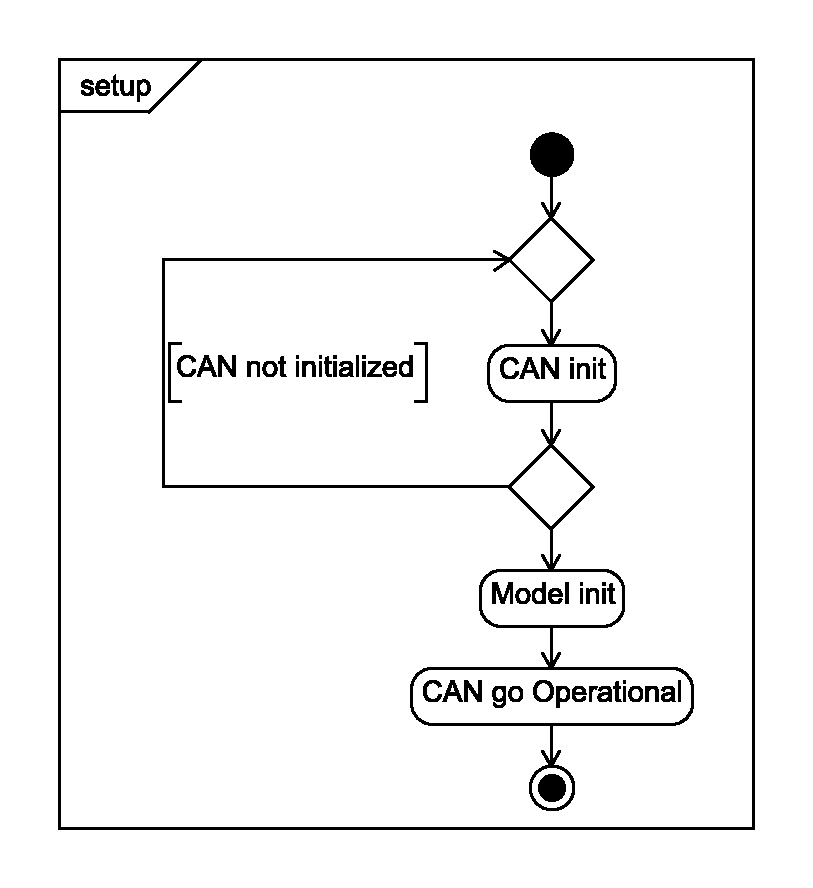
\includegraphics[width=10cm]{setup_activity}
\doxyfigcaption{Setup Activity}
\end{DoxyImage}


\begin{DoxyAuthor}{Author}
Arella Matteo ~\newline
 (mail\+: \href{mailto:arella.1646983@studenti.uniroma1.it}{\tt arella.\+1646983@studenti.\+uniroma1.\+it}) 
\end{DoxyAuthor}


Definition at line 48 of file V\+C\+U.\+ino.


\chapter{File Documentation}
\hypertarget{board__pinout_8h}{}\section{board\+\_\+pinout.\+h File Reference}
\label{board__pinout_8h}\index{board\+\_\+pinout.\+h@{board\+\_\+pinout.\+h}}
\subsection*{Macros}
\begin{DoxyCompactItemize}
\item 
\#define \mbox{\hyperlink{board__pinout_8h_aea8caf3e051442ba02c4e44a59602796}{C\+A\+N\+\_\+\+F\+U\+N\+Z\+I\+O\+N\+A\+LE}}~Can1
\item 
\#define \mbox{\hyperlink{board__pinout_8h_a8d2f70cd4c07aafe94fd9944121922d9}{C\+A\+N\+\_\+\+S\+E\+R\+V\+I\+ZI}}~Can0
\item 
\#define \mbox{\hyperlink{board__pinout_8h_a15003800bba3fb64e770c6a920613419}{A\+I\+Rcc}}~48
\item 
\#define \mbox{\hyperlink{board__pinout_8h_ab421578437964f5c645163739a0803e7}{A\+I\+R\+Gnd}}~49
\item 
\#define \mbox{\hyperlink{board__pinout_8h_a349316092037fdd0773335fab4e15ee8}{P\+RE}}~47
\item 
\#define \mbox{\hyperlink{board__pinout_8h_a145103118f6d9d1129aa4509cf214a13}{B\+U\+Z\+Z\+ER}}~52
\item 
\#define \mbox{\hyperlink{board__pinout_8h_a78a99c4f7bcb7723d7bf21810c4ce09b}{A\+I\+RB}}~14
\item 
\#define \mbox{\hyperlink{board__pinout_8h_a1bcd7461cf494d3235f792bf3d814923}{R\+T\+DB}}~15
\item 
\#define \mbox{\hyperlink{board__pinout_8h_acd9448edb89c378d843fc3cb93a098d3}{F\+AN}}~9
\item 
\#define \mbox{\hyperlink{board__pinout_8h_ad6c9e9b63f53c664772ee858436e0ae9}{I\+N\+V\+E\+R\+T\+E\+R\+\_\+\+A\+N\+A\+L\+O\+G\+\_\+\+P\+IN}}~D\+A\+C1
\item 
\#define \mbox{\hyperlink{board__pinout_8h_a604c7f4c9fe74f1d9877071bbee1c9e0}{B\+R\+A\+K\+E\+\_\+\+R\+E\+G\+E\+N\+\_\+\+P\+IN}}~D\+A\+C0
\item 
\#define \mbox{\hyperlink{board__pinout_8h_ae9aa914854f611488701c96a330b0bd4}{T\+P\+S1\+\_\+\+P\+IN}}~A0
\item 
\#define \mbox{\hyperlink{board__pinout_8h_a99b2a7dadaf495e3c559a46440f9141f}{T\+P\+S1\+\_\+\+A\+D\+C\+\_\+\+C\+H\+A\+N\+\_\+\+N\+UM}}~A\+D\+C\+\_\+\+C\+H\+E\+R\+\_\+\+C\+H7
\item 
\#define \mbox{\hyperlink{board__pinout_8h_ab13a816bae3ca994897fc6f1cb590a67}{T\+P\+S2\+\_\+\+P\+IN}}~A1
\item 
\#define \mbox{\hyperlink{board__pinout_8h_a4cecb8c10512873904099a1a88d69ed3}{T\+P\+S2\+\_\+\+A\+D\+C\+\_\+\+C\+H\+A\+N\+\_\+\+N\+UM}}~A\+D\+C\+\_\+\+C\+H\+E\+R\+\_\+\+C\+H6
\item 
\#define \mbox{\hyperlink{board__pinout_8h_ad632b56bf4c6259a390c3db91607078e}{B\+R\+A\+K\+E\+\_\+\+P\+IN}}~A2
\item 
\#define \mbox{\hyperlink{board__pinout_8h_a310547321c4a016c4ad19922920fadfd}{B\+R\+A\+K\+E\+\_\+\+A\+D\+C\+\_\+\+C\+H\+A\+N\+\_\+\+N\+UM}}~A\+D\+C\+\_\+\+C\+H\+E\+R\+\_\+\+C\+H5
\item 
\#define \mbox{\hyperlink{board__pinout_8h_abbdb157ae4ad39d102935c21fa30d1c5}{S\+C\+\_\+\+P\+IN}}~A3
\item 
\#define \mbox{\hyperlink{board__pinout_8h_a564adb575db2620ac85e3abdd6a5bbaf}{S\+C\+\_\+\+A\+D\+C\+\_\+\+C\+H\+A\+N\+\_\+\+N\+UM}}~A\+D\+C\+\_\+\+C\+H\+E\+R\+\_\+\+C\+H4
\end{DoxyCompactItemize}


\subsection{Macro Definition Documentation}
\mbox{\Hypertarget{board__pinout_8h_a78a99c4f7bcb7723d7bf21810c4ce09b}\label{board__pinout_8h_a78a99c4f7bcb7723d7bf21810c4ce09b}} 
\index{board\+\_\+pinout.\+h@{board\+\_\+pinout.\+h}!A\+I\+RB@{A\+I\+RB}}
\index{A\+I\+RB@{A\+I\+RB}!board\+\_\+pinout.\+h@{board\+\_\+pinout.\+h}}
\subsubsection{\texorpdfstring{A\+I\+RB}{AIRB}}
{\footnotesize\ttfamily \#define A\+I\+RB~14}



Definition at line 11 of file board\+\_\+pinout.\+h.

\mbox{\Hypertarget{board__pinout_8h_a15003800bba3fb64e770c6a920613419}\label{board__pinout_8h_a15003800bba3fb64e770c6a920613419}} 
\index{board\+\_\+pinout.\+h@{board\+\_\+pinout.\+h}!A\+I\+Rcc@{A\+I\+Rcc}}
\index{A\+I\+Rcc@{A\+I\+Rcc}!board\+\_\+pinout.\+h@{board\+\_\+pinout.\+h}}
\subsubsection{\texorpdfstring{A\+I\+Rcc}{AIRcc}}
{\footnotesize\ttfamily \#define A\+I\+Rcc~48}



Definition at line 7 of file board\+\_\+pinout.\+h.

\mbox{\Hypertarget{board__pinout_8h_ab421578437964f5c645163739a0803e7}\label{board__pinout_8h_ab421578437964f5c645163739a0803e7}} 
\index{board\+\_\+pinout.\+h@{board\+\_\+pinout.\+h}!A\+I\+R\+Gnd@{A\+I\+R\+Gnd}}
\index{A\+I\+R\+Gnd@{A\+I\+R\+Gnd}!board\+\_\+pinout.\+h@{board\+\_\+pinout.\+h}}
\subsubsection{\texorpdfstring{A\+I\+R\+Gnd}{AIRGnd}}
{\footnotesize\ttfamily \#define A\+I\+R\+Gnd~49}



Definition at line 8 of file board\+\_\+pinout.\+h.

\mbox{\Hypertarget{board__pinout_8h_a310547321c4a016c4ad19922920fadfd}\label{board__pinout_8h_a310547321c4a016c4ad19922920fadfd}} 
\index{board\+\_\+pinout.\+h@{board\+\_\+pinout.\+h}!B\+R\+A\+K\+E\+\_\+\+A\+D\+C\+\_\+\+C\+H\+A\+N\+\_\+\+N\+UM@{B\+R\+A\+K\+E\+\_\+\+A\+D\+C\+\_\+\+C\+H\+A\+N\+\_\+\+N\+UM}}
\index{B\+R\+A\+K\+E\+\_\+\+A\+D\+C\+\_\+\+C\+H\+A\+N\+\_\+\+N\+UM@{B\+R\+A\+K\+E\+\_\+\+A\+D\+C\+\_\+\+C\+H\+A\+N\+\_\+\+N\+UM}!board\+\_\+pinout.\+h@{board\+\_\+pinout.\+h}}
\subsubsection{\texorpdfstring{B\+R\+A\+K\+E\+\_\+\+A\+D\+C\+\_\+\+C\+H\+A\+N\+\_\+\+N\+UM}{BRAKE\_ADC\_CHAN\_NUM}}
{\footnotesize\ttfamily \#define B\+R\+A\+K\+E\+\_\+\+A\+D\+C\+\_\+\+C\+H\+A\+N\+\_\+\+N\+UM~A\+D\+C\+\_\+\+C\+H\+E\+R\+\_\+\+C\+H5}



Definition at line 25 of file board\+\_\+pinout.\+h.

\mbox{\Hypertarget{board__pinout_8h_ad632b56bf4c6259a390c3db91607078e}\label{board__pinout_8h_ad632b56bf4c6259a390c3db91607078e}} 
\index{board\+\_\+pinout.\+h@{board\+\_\+pinout.\+h}!B\+R\+A\+K\+E\+\_\+\+P\+IN@{B\+R\+A\+K\+E\+\_\+\+P\+IN}}
\index{B\+R\+A\+K\+E\+\_\+\+P\+IN@{B\+R\+A\+K\+E\+\_\+\+P\+IN}!board\+\_\+pinout.\+h@{board\+\_\+pinout.\+h}}
\subsubsection{\texorpdfstring{B\+R\+A\+K\+E\+\_\+\+P\+IN}{BRAKE\_PIN}}
{\footnotesize\ttfamily \#define B\+R\+A\+K\+E\+\_\+\+P\+IN~A2}



Definition at line 24 of file board\+\_\+pinout.\+h.

\mbox{\Hypertarget{board__pinout_8h_a604c7f4c9fe74f1d9877071bbee1c9e0}\label{board__pinout_8h_a604c7f4c9fe74f1d9877071bbee1c9e0}} 
\index{board\+\_\+pinout.\+h@{board\+\_\+pinout.\+h}!B\+R\+A\+K\+E\+\_\+\+R\+E\+G\+E\+N\+\_\+\+P\+IN@{B\+R\+A\+K\+E\+\_\+\+R\+E\+G\+E\+N\+\_\+\+P\+IN}}
\index{B\+R\+A\+K\+E\+\_\+\+R\+E\+G\+E\+N\+\_\+\+P\+IN@{B\+R\+A\+K\+E\+\_\+\+R\+E\+G\+E\+N\+\_\+\+P\+IN}!board\+\_\+pinout.\+h@{board\+\_\+pinout.\+h}}
\subsubsection{\texorpdfstring{B\+R\+A\+K\+E\+\_\+\+R\+E\+G\+E\+N\+\_\+\+P\+IN}{BRAKE\_REGEN\_PIN}}
{\footnotesize\ttfamily \#define B\+R\+A\+K\+E\+\_\+\+R\+E\+G\+E\+N\+\_\+\+P\+IN~D\+A\+C0}



Definition at line 16 of file board\+\_\+pinout.\+h.

\mbox{\Hypertarget{board__pinout_8h_a145103118f6d9d1129aa4509cf214a13}\label{board__pinout_8h_a145103118f6d9d1129aa4509cf214a13}} 
\index{board\+\_\+pinout.\+h@{board\+\_\+pinout.\+h}!B\+U\+Z\+Z\+ER@{B\+U\+Z\+Z\+ER}}
\index{B\+U\+Z\+Z\+ER@{B\+U\+Z\+Z\+ER}!board\+\_\+pinout.\+h@{board\+\_\+pinout.\+h}}
\subsubsection{\texorpdfstring{B\+U\+Z\+Z\+ER}{BUZZER}}
{\footnotesize\ttfamily \#define B\+U\+Z\+Z\+ER~52}



Definition at line 10 of file board\+\_\+pinout.\+h.

\mbox{\Hypertarget{board__pinout_8h_aea8caf3e051442ba02c4e44a59602796}\label{board__pinout_8h_aea8caf3e051442ba02c4e44a59602796}} 
\index{board\+\_\+pinout.\+h@{board\+\_\+pinout.\+h}!C\+A\+N\+\_\+\+F\+U\+N\+Z\+I\+O\+N\+A\+LE@{C\+A\+N\+\_\+\+F\+U\+N\+Z\+I\+O\+N\+A\+LE}}
\index{C\+A\+N\+\_\+\+F\+U\+N\+Z\+I\+O\+N\+A\+LE@{C\+A\+N\+\_\+\+F\+U\+N\+Z\+I\+O\+N\+A\+LE}!board\+\_\+pinout.\+h@{board\+\_\+pinout.\+h}}
\subsubsection{\texorpdfstring{C\+A\+N\+\_\+\+F\+U\+N\+Z\+I\+O\+N\+A\+LE}{CAN\_FUNZIONALE}}
{\footnotesize\ttfamily \#define C\+A\+N\+\_\+\+F\+U\+N\+Z\+I\+O\+N\+A\+LE~Can1}



Definition at line 4 of file board\+\_\+pinout.\+h.

\mbox{\Hypertarget{board__pinout_8h_a8d2f70cd4c07aafe94fd9944121922d9}\label{board__pinout_8h_a8d2f70cd4c07aafe94fd9944121922d9}} 
\index{board\+\_\+pinout.\+h@{board\+\_\+pinout.\+h}!C\+A\+N\+\_\+\+S\+E\+R\+V\+I\+ZI@{C\+A\+N\+\_\+\+S\+E\+R\+V\+I\+ZI}}
\index{C\+A\+N\+\_\+\+S\+E\+R\+V\+I\+ZI@{C\+A\+N\+\_\+\+S\+E\+R\+V\+I\+ZI}!board\+\_\+pinout.\+h@{board\+\_\+pinout.\+h}}
\subsubsection{\texorpdfstring{C\+A\+N\+\_\+\+S\+E\+R\+V\+I\+ZI}{CAN\_SERVIZI}}
{\footnotesize\ttfamily \#define C\+A\+N\+\_\+\+S\+E\+R\+V\+I\+ZI~Can0}



Definition at line 5 of file board\+\_\+pinout.\+h.

\mbox{\Hypertarget{board__pinout_8h_acd9448edb89c378d843fc3cb93a098d3}\label{board__pinout_8h_acd9448edb89c378d843fc3cb93a098d3}} 
\index{board\+\_\+pinout.\+h@{board\+\_\+pinout.\+h}!F\+AN@{F\+AN}}
\index{F\+AN@{F\+AN}!board\+\_\+pinout.\+h@{board\+\_\+pinout.\+h}}
\subsubsection{\texorpdfstring{F\+AN}{FAN}}
{\footnotesize\ttfamily \#define F\+AN~9}



Definition at line 13 of file board\+\_\+pinout.\+h.

\mbox{\Hypertarget{board__pinout_8h_ad6c9e9b63f53c664772ee858436e0ae9}\label{board__pinout_8h_ad6c9e9b63f53c664772ee858436e0ae9}} 
\index{board\+\_\+pinout.\+h@{board\+\_\+pinout.\+h}!I\+N\+V\+E\+R\+T\+E\+R\+\_\+\+A\+N\+A\+L\+O\+G\+\_\+\+P\+IN@{I\+N\+V\+E\+R\+T\+E\+R\+\_\+\+A\+N\+A\+L\+O\+G\+\_\+\+P\+IN}}
\index{I\+N\+V\+E\+R\+T\+E\+R\+\_\+\+A\+N\+A\+L\+O\+G\+\_\+\+P\+IN@{I\+N\+V\+E\+R\+T\+E\+R\+\_\+\+A\+N\+A\+L\+O\+G\+\_\+\+P\+IN}!board\+\_\+pinout.\+h@{board\+\_\+pinout.\+h}}
\subsubsection{\texorpdfstring{I\+N\+V\+E\+R\+T\+E\+R\+\_\+\+A\+N\+A\+L\+O\+G\+\_\+\+P\+IN}{INVERTER\_ANALOG\_PIN}}
{\footnotesize\ttfamily \#define I\+N\+V\+E\+R\+T\+E\+R\+\_\+\+A\+N\+A\+L\+O\+G\+\_\+\+P\+IN~D\+A\+C1}



Definition at line 15 of file board\+\_\+pinout.\+h.

\mbox{\Hypertarget{board__pinout_8h_a349316092037fdd0773335fab4e15ee8}\label{board__pinout_8h_a349316092037fdd0773335fab4e15ee8}} 
\index{board\+\_\+pinout.\+h@{board\+\_\+pinout.\+h}!P\+RE@{P\+RE}}
\index{P\+RE@{P\+RE}!board\+\_\+pinout.\+h@{board\+\_\+pinout.\+h}}
\subsubsection{\texorpdfstring{P\+RE}{PRE}}
{\footnotesize\ttfamily \#define P\+RE~47}



Definition at line 9 of file board\+\_\+pinout.\+h.

\mbox{\Hypertarget{board__pinout_8h_a1bcd7461cf494d3235f792bf3d814923}\label{board__pinout_8h_a1bcd7461cf494d3235f792bf3d814923}} 
\index{board\+\_\+pinout.\+h@{board\+\_\+pinout.\+h}!R\+T\+DB@{R\+T\+DB}}
\index{R\+T\+DB@{R\+T\+DB}!board\+\_\+pinout.\+h@{board\+\_\+pinout.\+h}}
\subsubsection{\texorpdfstring{R\+T\+DB}{RTDB}}
{\footnotesize\ttfamily \#define R\+T\+DB~15}



Definition at line 12 of file board\+\_\+pinout.\+h.

\mbox{\Hypertarget{board__pinout_8h_a564adb575db2620ac85e3abdd6a5bbaf}\label{board__pinout_8h_a564adb575db2620ac85e3abdd6a5bbaf}} 
\index{board\+\_\+pinout.\+h@{board\+\_\+pinout.\+h}!S\+C\+\_\+\+A\+D\+C\+\_\+\+C\+H\+A\+N\+\_\+\+N\+UM@{S\+C\+\_\+\+A\+D\+C\+\_\+\+C\+H\+A\+N\+\_\+\+N\+UM}}
\index{S\+C\+\_\+\+A\+D\+C\+\_\+\+C\+H\+A\+N\+\_\+\+N\+UM@{S\+C\+\_\+\+A\+D\+C\+\_\+\+C\+H\+A\+N\+\_\+\+N\+UM}!board\+\_\+pinout.\+h@{board\+\_\+pinout.\+h}}
\subsubsection{\texorpdfstring{S\+C\+\_\+\+A\+D\+C\+\_\+\+C\+H\+A\+N\+\_\+\+N\+UM}{SC\_ADC\_CHAN\_NUM}}
{\footnotesize\ttfamily \#define S\+C\+\_\+\+A\+D\+C\+\_\+\+C\+H\+A\+N\+\_\+\+N\+UM~A\+D\+C\+\_\+\+C\+H\+E\+R\+\_\+\+C\+H4}



Definition at line 28 of file board\+\_\+pinout.\+h.

\mbox{\Hypertarget{board__pinout_8h_abbdb157ae4ad39d102935c21fa30d1c5}\label{board__pinout_8h_abbdb157ae4ad39d102935c21fa30d1c5}} 
\index{board\+\_\+pinout.\+h@{board\+\_\+pinout.\+h}!S\+C\+\_\+\+P\+IN@{S\+C\+\_\+\+P\+IN}}
\index{S\+C\+\_\+\+P\+IN@{S\+C\+\_\+\+P\+IN}!board\+\_\+pinout.\+h@{board\+\_\+pinout.\+h}}
\subsubsection{\texorpdfstring{S\+C\+\_\+\+P\+IN}{SC\_PIN}}
{\footnotesize\ttfamily \#define S\+C\+\_\+\+P\+IN~A3}



Definition at line 27 of file board\+\_\+pinout.\+h.

\mbox{\Hypertarget{board__pinout_8h_a99b2a7dadaf495e3c559a46440f9141f}\label{board__pinout_8h_a99b2a7dadaf495e3c559a46440f9141f}} 
\index{board\+\_\+pinout.\+h@{board\+\_\+pinout.\+h}!T\+P\+S1\+\_\+\+A\+D\+C\+\_\+\+C\+H\+A\+N\+\_\+\+N\+UM@{T\+P\+S1\+\_\+\+A\+D\+C\+\_\+\+C\+H\+A\+N\+\_\+\+N\+UM}}
\index{T\+P\+S1\+\_\+\+A\+D\+C\+\_\+\+C\+H\+A\+N\+\_\+\+N\+UM@{T\+P\+S1\+\_\+\+A\+D\+C\+\_\+\+C\+H\+A\+N\+\_\+\+N\+UM}!board\+\_\+pinout.\+h@{board\+\_\+pinout.\+h}}
\subsubsection{\texorpdfstring{T\+P\+S1\+\_\+\+A\+D\+C\+\_\+\+C\+H\+A\+N\+\_\+\+N\+UM}{TPS1\_ADC\_CHAN\_NUM}}
{\footnotesize\ttfamily \#define T\+P\+S1\+\_\+\+A\+D\+C\+\_\+\+C\+H\+A\+N\+\_\+\+N\+UM~A\+D\+C\+\_\+\+C\+H\+E\+R\+\_\+\+C\+H7}



Definition at line 19 of file board\+\_\+pinout.\+h.

\mbox{\Hypertarget{board__pinout_8h_ae9aa914854f611488701c96a330b0bd4}\label{board__pinout_8h_ae9aa914854f611488701c96a330b0bd4}} 
\index{board\+\_\+pinout.\+h@{board\+\_\+pinout.\+h}!T\+P\+S1\+\_\+\+P\+IN@{T\+P\+S1\+\_\+\+P\+IN}}
\index{T\+P\+S1\+\_\+\+P\+IN@{T\+P\+S1\+\_\+\+P\+IN}!board\+\_\+pinout.\+h@{board\+\_\+pinout.\+h}}
\subsubsection{\texorpdfstring{T\+P\+S1\+\_\+\+P\+IN}{TPS1\_PIN}}
{\footnotesize\ttfamily \#define T\+P\+S1\+\_\+\+P\+IN~A0}



Definition at line 18 of file board\+\_\+pinout.\+h.

\mbox{\Hypertarget{board__pinout_8h_a4cecb8c10512873904099a1a88d69ed3}\label{board__pinout_8h_a4cecb8c10512873904099a1a88d69ed3}} 
\index{board\+\_\+pinout.\+h@{board\+\_\+pinout.\+h}!T\+P\+S2\+\_\+\+A\+D\+C\+\_\+\+C\+H\+A\+N\+\_\+\+N\+UM@{T\+P\+S2\+\_\+\+A\+D\+C\+\_\+\+C\+H\+A\+N\+\_\+\+N\+UM}}
\index{T\+P\+S2\+\_\+\+A\+D\+C\+\_\+\+C\+H\+A\+N\+\_\+\+N\+UM@{T\+P\+S2\+\_\+\+A\+D\+C\+\_\+\+C\+H\+A\+N\+\_\+\+N\+UM}!board\+\_\+pinout.\+h@{board\+\_\+pinout.\+h}}
\subsubsection{\texorpdfstring{T\+P\+S2\+\_\+\+A\+D\+C\+\_\+\+C\+H\+A\+N\+\_\+\+N\+UM}{TPS2\_ADC\_CHAN\_NUM}}
{\footnotesize\ttfamily \#define T\+P\+S2\+\_\+\+A\+D\+C\+\_\+\+C\+H\+A\+N\+\_\+\+N\+UM~A\+D\+C\+\_\+\+C\+H\+E\+R\+\_\+\+C\+H6}



Definition at line 22 of file board\+\_\+pinout.\+h.

\mbox{\Hypertarget{board__pinout_8h_ab13a816bae3ca994897fc6f1cb590a67}\label{board__pinout_8h_ab13a816bae3ca994897fc6f1cb590a67}} 
\index{board\+\_\+pinout.\+h@{board\+\_\+pinout.\+h}!T\+P\+S2\+\_\+\+P\+IN@{T\+P\+S2\+\_\+\+P\+IN}}
\index{T\+P\+S2\+\_\+\+P\+IN@{T\+P\+S2\+\_\+\+P\+IN}!board\+\_\+pinout.\+h@{board\+\_\+pinout.\+h}}
\subsubsection{\texorpdfstring{T\+P\+S2\+\_\+\+P\+IN}{TPS2\_PIN}}
{\footnotesize\ttfamily \#define T\+P\+S2\+\_\+\+P\+IN~A1}



Definition at line 21 of file board\+\_\+pinout.\+h.


\hypertarget{can__funzionale_8cpp}{\section{can\-\_\-funzionale.\-cpp File Reference}
\label{can__funzionale_8cpp}\index{can\-\_\-funzionale.\-cpp@{can\-\_\-funzionale.\-cpp}}
}


C\-A\-N funzionale module implementation.  


{\ttfamily \#include \char`\"{}can\-\_\-funzionale.\-h\char`\"{}}\\*
{\ttfamily \#include \char`\"{}def.\-h\char`\"{}}\\*
{\ttfamily \#include $<$due\-\_\-can.\-h$>$}\\*
{\ttfamily \#include $<$Due\-Timer.\-h$>$}\\*
\subsection*{Functions}
\begin{DoxyCompactItemize}
\item 
volatile bool \hyperlink{group___c_a_n__funzionale__group_gaf1acdfa5537f47656edd6ffa3e7c24bd}{can\-\_\-funzionale\-\_\-initialized} ()
\begin{DoxyCompactList}\small\item\em This function returns C\-A\-N funzionale initialization status. \end{DoxyCompactList}\item 
void \hyperlink{group___c_a_n__funzionale__group_gac93bbbf1b84f1bc82b26d54d7f898172}{can\-\_\-funzionale\-\_\-send\-\_\-sync} ()
\begin{DoxyCompactList}\small\item\em This function sends a periodic C\-A\-N\-Open sync message to inverter slave node. \end{DoxyCompactList}\item 
void \hyperlink{group___c_a_n__funzionale__group_gaf4990e00c0c4a9f9eeb9cb5bdaecfa94}{C\-A\-N\-\_\-\-F\-U\-N\-Z\-\_\-\-B\-O\-O\-T\-U\-P\-\_\-\-C\-B} (C\-A\-N\-\_\-\-F\-R\-A\-M\-E $\ast$frame)
\begin{DoxyCompactList}\small\item\em This function manage boot-\/up message sent over C\-A\-N funzionale network by inverter slave node. Upon boot-\/up message reception the V\-C\-U send a S\-D\-O client request for check inverter vendor I\-D; then inverter is considered online over C\-A\-N funzionale network. \end{DoxyCompactList}\item 
void \hyperlink{group___c_a_n__funzionale__group_ga81bbc4c65d579febfbcae399f0ecbffc}{C\-A\-N\-\_\-\-F\-U\-N\-Z\-\_\-\-V\-E\-N\-D\-O\-R\-\_\-\-I\-D\-\_\-\-C\-B} (C\-A\-N\-\_\-\-F\-R\-A\-M\-E $\ast$frame)
\begin{DoxyCompactList}\small\item\em This function manage S\-D\-O server response with inverter Vendor I\-D. V\-C\-U sends N\-M\-T operational and P\-D\-Os to enable P\-W\-M; then inverter is considered correctly configured and a timer is started for sending periodic sync messages. \end{DoxyCompactList}\item 
void \hyperlink{group___c_a_n__funzionale__group_ga1fcfa8e31cfbfe2461328c345b5b8e19}{C\-A\-N\-\_\-\-F\-U\-N\-Z\-\_\-\-G\-E\-N\-E\-R\-A\-L\-\_\-\-C\-B} (C\-A\-N\-\_\-\-F\-R\-A\-M\-E $\ast$frame)
\begin{DoxyCompactList}\small\item\em This function manage T\-P\-D\-O from inverter and deserializes data\-: \end{DoxyCompactList}\item 
bool \hyperlink{group___c_a_n__funzionale__group_ga578b28192b0c78942fcc0452d070accb}{can\-\_\-funzionale\-\_\-init} ()
\begin{DoxyCompactList}\small\item\em This function initialize C\-A\-N funzionale hardware port with baudrate \hyperlink{common_8h_adee7e3800c996a5a977034531d94570d}{C\-A\-N\-\_\-\-F\-U\-N\-Z\-\_\-\-B\-A\-U\-D\-R\-A\-T\-E}. Mailbox 0 is configured for receiving boot-\/up messages from inverter slave node (filter = 0x00000700 + \hyperlink{group___c_a_n__funzionale__group_ga59ea82aec4abe07072cbdad555a8c1b9}{I\-N\-V\-E\-R\-T\-E\-R\-\_\-\-N\-O\-D\-E\-\_\-\-I\-D}, mask = 0x1\-F\-F\-F\-F\-F\-F\-F); mailbox 1 is configured for receiving vendor\-I\-D S\-D\-O response from inverter (filter = 0x00000580 + \hyperlink{group___c_a_n__funzionale__group_ga59ea82aec4abe07072cbdad555a8c1b9}{I\-N\-V\-E\-R\-T\-E\-R\-\_\-\-N\-O\-D\-E\-\_\-\-I\-D}, mask = 0x1\-F\-F\-F\-F\-F\-F\-F); remaining mailboxes are configured for receiving T\-P\-D\-Os from inverter slave node (filter = 0x00000080, mask = 0x1\-F\-F\-F\-F\-C\-F\-F). \end{DoxyCompactList}\item 
volatile bool \hyperlink{group___c_a_n__funzionale__group_ga7d74fd826c5df3b86fd751f91c61671f}{can\-\_\-funzionale\-\_\-online} ()
\begin{DoxyCompactList}\small\item\em This function returns if inverter is online and active over C\-A\-N funzionale. \end{DoxyCompactList}\item 
void \hyperlink{group___c_a_n__funzionale__group_ga41854ab275f2b3cb7efb9385502d7d65}{inverter\-\_\-torque\-\_\-request} (uint16\-\_\-t torque)
\begin{DoxyCompactList}\small\item\em This function send torque request to inverter. If inverter is active over C\-A\-N funzionale network then the request is done via R\-P\-D\-O1 viceversa it's done via analog signal. \end{DoxyCompactList}\item 
void \hyperlink{group___c_a_n__funzionale__group_ga75820e0d72b7f264a70d99f414745518}{inverter\-\_\-regen\-\_\-request} (uint16\-\_\-t regen)
\begin{DoxyCompactList}\small\item\em This function send regen request to inverter. \end{DoxyCompactList}\item 
volatile uint16\-\_\-t \hyperlink{group___c_a_n__funzionale__group_ga3c4828f57a818b8e1b2f277c2174b5da}{get\-\_\-torque\-\_\-actual\-\_\-value} ()
\begin{DoxyCompactList}\small\item\em This function return the torque value requested by inverter to motor retrieved from T\-P\-D\-O1 from inverter over C\-A\-N funzionale network. \end{DoxyCompactList}\end{DoxyCompactItemize}
\subsection*{Variables}
\begin{DoxyCompactItemize}
\item 
\hypertarget{group___c_a_n__funzionale__group_ga8cd40fe9b965184307fe5886fcef6236}{volatile bool \hyperlink{group___c_a_n__funzionale__group_ga8cd40fe9b965184307fe5886fcef6236}{can\-\_\-funz\-\_\-initialized} = false}\label{group___c_a_n__funzionale__group_ga8cd40fe9b965184307fe5886fcef6236}

\begin{DoxyCompactList}\small\item\em C\-A\-N funzionale initialization status flag (true if initialized) \end{DoxyCompactList}\item 
\hypertarget{group___c_a_n__funzionale__group_ga392f688b1edd69f29b48818a5b9b19ae}{volatile bool \hyperlink{group___c_a_n__funzionale__group_ga392f688b1edd69f29b48818a5b9b19ae}{inverter\-\_\-online} = false}\label{group___c_a_n__funzionale__group_ga392f688b1edd69f29b48818a5b9b19ae}

\begin{DoxyCompactList}\small\item\em Inverter online status flag (true if online) \end{DoxyCompactList}\item 
\hypertarget{group___c_a_n__funzionale__group_ga979fff19d884e9a83eecc2309b36ad0c}{volatile bool \hyperlink{group___c_a_n__funzionale__group_ga979fff19d884e9a83eecc2309b36ad0c}{inverter\-\_\-configured} = false}\label{group___c_a_n__funzionale__group_ga979fff19d884e9a83eecc2309b36ad0c}

\begin{DoxyCompactList}\small\item\em Inverter configured status flag (true if configured) \end{DoxyCompactList}\item 
\hypertarget{group___c_a_n__funzionale__group_ga99ead1878913db87bc7cc808a8392e21}{volatile uint16\-\_\-t \hyperlink{group___c_a_n__funzionale__group_ga99ead1878913db87bc7cc808a8392e21}{torque\-\_\-actual\-\_\-value} = 0}\label{group___c_a_n__funzionale__group_ga99ead1878913db87bc7cc808a8392e21}

\begin{DoxyCompactList}\small\item\em Torque requested by inverter to motor. \end{DoxyCompactList}\end{DoxyCompactItemize}


\subsection{Detailed Description}
C\-A\-N funzionale module implementation. \begin{DoxyAuthor}{Author}
Arella Matteo \par
 (mail\-: \href{mailto:arella.1646983@studenti.uniroma1.it}{\tt arella.\-1646983@studenti.\-uniroma1.\-it}) 
\end{DoxyAuthor}
\begin{DoxyDate}{Date}
2018 
\end{DoxyDate}


Definition in file \hyperlink{can__funzionale_8cpp_source}{can\-\_\-funzionale.\-cpp}.


\hypertarget{can__funzionale_8h}{}\section{can\+\_\+funzionale.\+h File Reference}
\label{can__funzionale_8h}\index{can\+\_\+funzionale.\+h@{can\+\_\+funzionale.\+h}}


C\+AN funzionale module header.  


{\ttfamily \#include \char`\"{}common.\+h\char`\"{}}\newline
\subsection*{Functions}
\begin{DoxyCompactItemize}
\item 
bool \mbox{\hyperlink{group___c_a_n__funzionale__group_ga578b28192b0c78942fcc0452d070accb}{can\+\_\+funzionale\+\_\+init}} ()
\begin{DoxyCompactList}\small\item\em This function initialize C\+AN funzionale hardware port with baudrate \mbox{\hyperlink{common_8h_adee7e3800c996a5a977034531d94570d}{C\+A\+N\+\_\+\+F\+U\+N\+Z\+\_\+\+B\+A\+U\+D\+R\+A\+TE}}. Mailbox 0 is configured for receiving boot-\/up messages from inverter slave node (filter = 0x00000700 + \mbox{\hyperlink{group___c_a_n__funzionale__group_ga59ea82aec4abe07072cbdad555a8c1b9}{I\+N\+V\+E\+R\+T\+E\+R\+\_\+\+N\+O\+D\+E\+\_\+\+ID}}, mask = 0x1\+F\+F\+F\+F\+F\+FF); mailbox 1 is configured for receiving vendor\+ID S\+DO response from inverter (filter = 0x00000580 + \mbox{\hyperlink{group___c_a_n__funzionale__group_ga59ea82aec4abe07072cbdad555a8c1b9}{I\+N\+V\+E\+R\+T\+E\+R\+\_\+\+N\+O\+D\+E\+\_\+\+ID}}, mask = 0x1\+F\+F\+F\+F\+F\+FF); remaining mailboxes are configured for receiving T\+P\+D\+Os from inverter slave node (filter = 0x00000080, mask = 0x1\+F\+F\+F\+F\+C\+FF). \end{DoxyCompactList}\item 
volatile bool \mbox{\hyperlink{group___c_a_n__funzionale__group_gaf1acdfa5537f47656edd6ffa3e7c24bd}{can\+\_\+funzionale\+\_\+initialized}} ()
\begin{DoxyCompactList}\small\item\em This function returns C\+AN funzionale initialization status. \end{DoxyCompactList}\item 
volatile bool \mbox{\hyperlink{group___c_a_n__funzionale__group_ga7d74fd826c5df3b86fd751f91c61671f}{can\+\_\+funzionale\+\_\+online}} ()
\begin{DoxyCompactList}\small\item\em This function returns if inverter is online and active over C\+AN funzionale. \end{DoxyCompactList}\item 
void \mbox{\hyperlink{group___c_a_n__funzionale__group_ga41854ab275f2b3cb7efb9385502d7d65}{inverter\+\_\+torque\+\_\+request}} (uint16\+\_\+t torque)
\begin{DoxyCompactList}\small\item\em This function send torque request to inverter. If inverter is active over C\+AN funzionale network then the request is done via R\+P\+D\+O1 viceversa it\textquotesingle{}s done via analog signal. \end{DoxyCompactList}\item 
void \mbox{\hyperlink{group___c_a_n__funzionale__group_ga75820e0d72b7f264a70d99f414745518}{inverter\+\_\+regen\+\_\+request}} (uint16\+\_\+t regen)
\begin{DoxyCompactList}\small\item\em This function send regen request to inverter. \end{DoxyCompactList}\item 
volatile uint16\+\_\+t \mbox{\hyperlink{group___c_a_n__funzionale__group_ga3c4828f57a818b8e1b2f277c2174b5da}{get\+\_\+torque\+\_\+actual\+\_\+value}} ()
\begin{DoxyCompactList}\small\item\em This function return the torque value requested by inverter to motor retrieved from T\+P\+D\+O1 from inverter over C\+AN funzionale network. \end{DoxyCompactList}\end{DoxyCompactItemize}


\subsection{Detailed Description}
C\+AN funzionale module header. 

\begin{DoxyAuthor}{Author}
Arella Matteo ~\newline
 (mail\+: \href{mailto:arella.1646983@studenti.uniroma1.it}{\tt arella.\+1646983@studenti.\+uniroma1.\+it}) 
\end{DoxyAuthor}
\begin{DoxyDate}{Date}
2018 
\end{DoxyDate}

\hypertarget{_c_a_n___i_d_8h}{\section{C\-A\-N\-\_\-\-I\-D.\-h File Reference}
\label{_c_a_n___i_d_8h}\index{C\-A\-N\-\_\-\-I\-D.\-h@{C\-A\-N\-\_\-\-I\-D.\-h}}
}


C\-A\-N nodes I\-D definitions module.  


\subsection*{Macros}
\begin{DoxyCompactItemize}
\item 
\hypertarget{group___c_a_n__module__group_ga5703fd8de5ab8d0dcedb561f2178829e}{\#define \hyperlink{group___c_a_n__module__group_ga5703fd8de5ab8d0dcedb561f2178829e}{V\-C\-U\-\_\-\-N\-O\-D\-E\-\_\-\-I\-D}~2}\label{group___c_a_n__module__group_ga5703fd8de5ab8d0dcedb561f2178829e}

\begin{DoxyCompactList}\small\item\em V\-C\-U Node I\-D. \end{DoxyCompactList}\item 
\hypertarget{group___c_a_n__funzionale__group_ga59ea82aec4abe07072cbdad555a8c1b9}{\#define \hyperlink{group___c_a_n__funzionale__group_ga59ea82aec4abe07072cbdad555a8c1b9}{I\-N\-V\-E\-R\-T\-E\-R\-\_\-\-N\-O\-D\-E\-\_\-\-I\-D}~1}\label{group___c_a_n__funzionale__group_ga59ea82aec4abe07072cbdad555a8c1b9}

\begin{DoxyCompactList}\small\item\em Inverter Node I\-D. \end{DoxyCompactList}\item 
\hypertarget{group___c_a_n__servizi__group_ga8d64b6b4c0f02ebded5440c6250e03b9}{\#define \hyperlink{group___c_a_n__servizi__group_ga8d64b6b4c0f02ebded5440c6250e03b9}{S\-C\-U\-\_\-\-F\-R\-O\-N\-T\-A\-L\-\_\-\-N\-O\-D\-E\-\_\-\-I\-D}~1}\label{group___c_a_n__servizi__group_ga8d64b6b4c0f02ebded5440c6250e03b9}

\begin{DoxyCompactList}\small\item\em Frontal S\-C\-U Node I\-D. \end{DoxyCompactList}\item 
\hypertarget{group___c_a_n__servizi__group_gaceef3f7366b39e88d89cb98ad8094c7b}{\#define \hyperlink{group___c_a_n__servizi__group_gaceef3f7366b39e88d89cb98ad8094c7b}{T\-C\-U\-\_\-\-N\-O\-D\-E\-\_\-\-I\-D}~4}\label{group___c_a_n__servizi__group_gaceef3f7366b39e88d89cb98ad8094c7b}

\begin{DoxyCompactList}\small\item\em T\-C\-U Node I\-D. \end{DoxyCompactList}\end{DoxyCompactItemize}


\subsection{Detailed Description}
C\-A\-N nodes I\-D definitions module. \begin{DoxyAuthor}{Author}
Arella Matteo \par
 (mail\-: \href{mailto:arella.1646983@studenti.uniroma1.it}{\tt arella.\-1646983@studenti.\-uniroma1.\-it}) 
\end{DoxyAuthor}
\begin{DoxyDate}{Date}
2018 
\end{DoxyDate}


Definition in file \hyperlink{_c_a_n___i_d_8h_source}{C\-A\-N\-\_\-\-I\-D.\-h}.


\hypertarget{can__servizi_8cpp}{\section{can\-\_\-servizi.\-cpp File Reference}
\label{can__servizi_8cpp}\index{can\-\_\-servizi.\-cpp@{can\-\_\-servizi.\-cpp}}
}


C\-A\-N servizi module implementation.  


{\ttfamily \#include \char`\"{}can\-\_\-servizi.\-h\char`\"{}}\\*
{\ttfamily \#include $<$due\-\_\-can.\-h$>$}\\*
{\ttfamily \#include $<$Due\-Timer.\-h$>$}\\*
\subsection*{Functions}
\begin{DoxyCompactItemize}
\item 
void \hyperlink{group___c_a_n__servizi__group_gad446b5782bcb2d8ffc0aa1f8c4d16ded}{timeout} ()
\begin{DoxyCompactList}\small\item\em This function is executed periodically after C\-A\-N servizi 'go Operational' N\-M\-T request is sent. When timeout occurs if \hyperlink{group___c_a_n__servizi__group_gadcbd4ad67b50cf61731266bf5c5ba158}{next\-\_\-pedals\-\_\-seq\-\_\-num} is greater than \hyperlink{group___c_a_n__servizi__group_gacad002b7cb06bffa8811859e6f53cb28}{curr\-\_\-pedals\-\_\-seq\-\_\-num} then frontal S\-C\-U is considered active, viceversa it is considered offline. \end{DoxyCompactList}\item 
volatile bool \hyperlink{group___c_a_n__servizi__group_gaa460928ec03256a076ebafceab10c2be}{can\-\_\-servizi\-\_\-initialized} ()
\begin{DoxyCompactList}\small\item\em This function returns C\-A\-N servizi initialization status. \end{DoxyCompactList}\item 
void \hyperlink{group___c_a_n__servizi__group_gaab9a1dbabaf97e474f5597e8b2a02c6e}{C\-A\-N\-\_\-\-S\-E\-R\-V\-\_\-\-B\-O\-O\-T\-U\-P\-\_\-\-C\-B} (C\-A\-N\-\_\-\-F\-R\-A\-M\-E $\ast$frame)
\begin{DoxyCompactList}\small\item\em This function manage boot-\/up messages sent over C\-A\-N servizi network by slave nodes. \end{DoxyCompactList}\item 
void \hyperlink{group___c_a_n__servizi__group_ga5897a28288e24aa5131ff5b81f5fedc8}{C\-A\-N\-\_\-\-S\-E\-R\-V\-\_\-\-G\-E\-N\-E\-R\-A\-L\-\_\-\-C\-B} (C\-A\-N\-\_\-\-F\-R\-A\-M\-E $\ast$frame)
\begin{DoxyCompactList}\small\item\em This function manage P\-D\-Os received over C\-A\-N servizi network and deserializes data\-: \end{DoxyCompactList}\item 
bool \hyperlink{group___c_a_n__servizi__group_ga2d29bd107e96ae1986e8874f004ffc84}{can\-\_\-servizi\-\_\-init} ()
\begin{DoxyCompactList}\small\item\em This function initialize C\-A\-N servizi hardware port with baudrate \hyperlink{common_8h_a2a5e84dfc7fa972b75e7ddbc6cc52a45}{C\-A\-N\-\_\-\-S\-E\-R\-V\-\_\-\-B\-A\-U\-D\-R\-A\-T\-E}. Mailbox 0 is configured for receiving boot-\/up messages from C\-A\-N servizi slave nodes (filter = 0x00000700, mask = 0x1\-F\-F\-F\-F\-F80); remaining mailboxes are configured for receiving T\-P\-D\-Os from C\-A\-N servizi slave nodes (filter = 0x00000080, mask = 0x1\-F\-F\-F\-F\-C80). \end{DoxyCompactList}\item 
void \hyperlink{group___c_a_n__servizi__group_gad444fb6be3b439dcfbefff66e85efd94}{can\-\_\-servizi\-\_\-go\-\_\-operational} ()
\begin{DoxyCompactList}\small\item\em This function send a C\-A\-N\-Open master N\-M\-T message for request 'go to Operational' state to C\-A\-N servizi slave nodes (S\-C\-Us and T\-C\-U). \end{DoxyCompactList}\item 
volatile bool \hyperlink{group___c_a_n__servizi__group_ga43e9ef52770f760c5751d83b138c7e6b}{can\-\_\-servizi\-\_\-online} ()
\begin{DoxyCompactList}\small\item\em This function returns if C\-A\-N servizi network is online. \end{DoxyCompactList}\item 
volatile bool \hyperlink{group___c_a_n__servizi__group_ga0c5f72386ae62e3e0b6908efa2fb2b28}{tcs\-\_\-online} ()
\begin{DoxyCompactList}\small\item\em This function returns if T\-C\-U node is active and online on the C\-A\-N servizi network. \end{DoxyCompactList}\item 
volatile uint8\-\_\-t \hyperlink{group___c_a_n__servizi__group_gac899876f81f391e2daafcd8b22d2f32e}{get\-\_\-servizi\-\_\-tps1} ()
\begin{DoxyCompactList}\small\item\em This function returns the value of the first A\-P\-P\-S in percentage, retrieved by frontal S\-C\-U node over C\-A\-N servizi network. \end{DoxyCompactList}\item 
volatile uint8\-\_\-t \hyperlink{group___c_a_n__servizi__group_ga431b31efe978864b1a2db0d57a5b572a}{get\-\_\-servizi\-\_\-tps2} ()
\begin{DoxyCompactList}\small\item\em This function returns the value of the second A\-P\-P\-S in percentage, retrieved by frontal S\-C\-U node over C\-A\-N servizi network. \end{DoxyCompactList}\item 
volatile uint8\-\_\-t \hyperlink{group___c_a_n__servizi__group_ga21c09880bef645f24962658ef3dbb16e}{get\-\_\-servizi\-\_\-brake} ()
\begin{DoxyCompactList}\small\item\em This function returns the value of brake pedal position sensor in percentage, retrieved by frontal S\-C\-U node over C\-A\-N servizi network. \end{DoxyCompactList}\item 
volatile bool \hyperlink{group___c_a_n__servizi__group_ga66135a8978149fc6fa0b62446131ce95}{get\-\_\-servizi\-\_\-apps\-\_\-plausibility} ()
\begin{DoxyCompactList}\small\item\em This function returns the value of A\-P\-P\-S plausibility retrieved by frontal S\-C\-U node over C\-A\-N servizi network. \end{DoxyCompactList}\item 
volatile bool \hyperlink{group___c_a_n__servizi__group_ga064fdc5f825b2d50b1b13509e3f135d2}{get\-\_\-servizi\-\_\-brake\-\_\-plausibility} ()
\begin{DoxyCompactList}\small\item\em This function returns the value of brake plausibility retrieved by frontal S\-C\-U node over C\-A\-N servizi network. \end{DoxyCompactList}\item 
volatile uint8\-\_\-t \hyperlink{group___c_a_n__servizi__group_ga68bca94de95a77a3366f46eed661193f}{get\-\_\-tcs\-\_\-torque\-\_\-coefficient} ()
\begin{DoxyCompactList}\small\item\em This function returns the value of torque limiter percentage retrieved by T\-C\-U node over C\-A\-N servizi network. \end{DoxyCompactList}\end{DoxyCompactItemize}
\subsection*{Variables}
\begin{DoxyCompactItemize}
\item 
\hypertarget{group___c_a_n__servizi__group_gaf351ebc02b2d28174f8e4b18ff9edf5f}{volatile bool \hyperlink{group___c_a_n__servizi__group_gaf351ebc02b2d28174f8e4b18ff9edf5f}{can\-\_\-serv\-\_\-initialized} = false}\label{group___c_a_n__servizi__group_gaf351ebc02b2d28174f8e4b18ff9edf5f}

\begin{DoxyCompactList}\small\item\em C\-A\-N servizi initialization status flag (true if initialized) \end{DoxyCompactList}\item 
\hypertarget{group___c_a_n__servizi__group_gafc26efcf97051372e70a8d0f2f0c79f0}{volatile bool \hyperlink{group___c_a_n__servizi__group_gafc26efcf97051372e70a8d0f2f0c79f0}{S\-C\-U\-\_\-\-F\-\_\-online} = false}\label{group___c_a_n__servizi__group_gafc26efcf97051372e70a8d0f2f0c79f0}

\begin{DoxyCompactList}\small\item\em Frontal S\-C\-U online status flag (true if online) \end{DoxyCompactList}\item 
\hypertarget{group___c_a_n__servizi__group_gad3e88db55b4105026b7e451f853a796b}{volatile bool \hyperlink{group___c_a_n__servizi__group_gad3e88db55b4105026b7e451f853a796b}{T\-C\-S\-\_\-online} = false}\label{group___c_a_n__servizi__group_gad3e88db55b4105026b7e451f853a796b}

\begin{DoxyCompactList}\small\item\em T\-C\-S online status flag (true if online) \end{DoxyCompactList}\item 
\hypertarget{group___c_a_n__servizi__group_gacad002b7cb06bffa8811859e6f53cb28}{volatile uint32\-\_\-t \hyperlink{group___c_a_n__servizi__group_gacad002b7cb06bffa8811859e6f53cb28}{curr\-\_\-pedals\-\_\-seq\-\_\-num} = 0}\label{group___c_a_n__servizi__group_gacad002b7cb06bffa8811859e6f53cb28}

\begin{DoxyCompactList}\small\item\em Frontal S\-C\-U P\-D\-Otx1 current sequence number. \end{DoxyCompactList}\item 
\hypertarget{group___c_a_n__servizi__group_gadcbd4ad67b50cf61731266bf5c5ba158}{volatile uint32\-\_\-t \hyperlink{group___c_a_n__servizi__group_gadcbd4ad67b50cf61731266bf5c5ba158}{next\-\_\-pedals\-\_\-seq\-\_\-num} = 0}\label{group___c_a_n__servizi__group_gadcbd4ad67b50cf61731266bf5c5ba158}

\begin{DoxyCompactList}\small\item\em Frontal S\-C\-U P\-D\-Otx1 next sequence number. \end{DoxyCompactList}\item 
volatile uint8\-\_\-t \hyperlink{group___c_a_n__servizi__group_ga1d42f28ccf027a3243fad064fa47ef81}{tps1\-\_\-percentage} = 0
\begin{DoxyCompactList}\small\item\em First A\-P\-P\-S percentage value retrieved by frontal S\-C\-U node. \end{DoxyCompactList}\item 
volatile uint8\-\_\-t \hyperlink{group___c_a_n__servizi__group_gaf69d82f83885abc5adbd5fcbf4c421cf}{tps2\-\_\-percentage} = 0
\begin{DoxyCompactList}\small\item\em Second A\-P\-P\-S percentage value retrieved by frontal S\-C\-U node. \end{DoxyCompactList}\item 
volatile uint8\-\_\-t \hyperlink{group___c_a_n__servizi__group_ga8e50a30864da7026531520887968d4c0}{brake\-\_\-percentage} = 0
\begin{DoxyCompactList}\small\item\em Brake pedal position sensor percentage value retrieved by frontal S\-C\-U node. \end{DoxyCompactList}\item 
\hypertarget{group___c_a_n__servizi__group_gaa9de48f5a49bc92a608ed315c087f3a6}{volatile bool \hyperlink{group___c_a_n__servizi__group_gaa9de48f5a49bc92a608ed315c087f3a6}{apps\-\_\-plausibility} = true}\label{group___c_a_n__servizi__group_gaa9de48f5a49bc92a608ed315c087f3a6}

\begin{DoxyCompactList}\small\item\em A\-P\-P\-S plausibility status retrieved by frontal S\-C\-U node. \end{DoxyCompactList}\item 
\hypertarget{group___c_a_n__servizi__group_gae505d69d6ac9d4e7e3c2268ca6cb20b3}{volatile bool \hyperlink{group___c_a_n__servizi__group_gae505d69d6ac9d4e7e3c2268ca6cb20b3}{brake\-\_\-plausibility} = true}\label{group___c_a_n__servizi__group_gae505d69d6ac9d4e7e3c2268ca6cb20b3}

\begin{DoxyCompactList}\small\item\em Brake plausibility status retrieved by frontal S\-C\-U node. \end{DoxyCompactList}\item 
\hypertarget{group___c_a_n__servizi__group_gac6f04deffa2553115dad7c8b45e14d8b}{volatile uint8\-\_\-t \hyperlink{group___c_a_n__servizi__group_gac6f04deffa2553115dad7c8b45e14d8b}{tcs\-\_\-coefficient} = 0}\label{group___c_a_n__servizi__group_gac6f04deffa2553115dad7c8b45e14d8b}

\begin{DoxyCompactList}\small\item\em torque limiter percentage retrieved by T\-C\-U node \end{DoxyCompactList}\end{DoxyCompactItemize}


\subsection{Detailed Description}
C\-A\-N servizi module implementation. \begin{DoxyAuthor}{Author}
Arella Matteo \par
 (mail\-: \href{mailto:arella.1646983@studenti.uniroma1.it}{\tt arella.\-1646983@studenti.\-uniroma1.\-it}) 
\end{DoxyAuthor}
\begin{DoxyDate}{Date}
2018 
\end{DoxyDate}


Definition in file \hyperlink{can__servizi_8cpp_source}{can\-\_\-servizi.\-cpp}.


\hypertarget{can__servizi_8h}{}\section{can\+\_\+servizi.\+h File Reference}
\label{can__servizi_8h}\index{can\+\_\+servizi.\+h@{can\+\_\+servizi.\+h}}


C\+AN servizi module header.  


{\ttfamily \#include \char`\"{}common.\+h\char`\"{}}\newline
Include dependency graph for can\+\_\+servizi.\+h\+:\nopagebreak
\begin{figure}[H]
\begin{center}
\leavevmode
\includegraphics[width=305pt]{can__servizi_8h__incl}
\end{center}
\end{figure}
This graph shows which files directly or indirectly include this file\+:\nopagebreak
\begin{figure}[H]
\begin{center}
\leavevmode
\includegraphics[width=350pt]{can__servizi_8h__dep__incl}
\end{center}
\end{figure}
\subsection*{Functions}
\begin{DoxyCompactItemize}
\item 
bool \mbox{\hyperlink{group___c_a_n__servizi__group_ga2d29bd107e96ae1986e8874f004ffc84}{can\+\_\+servizi\+\_\+init}} ()
\begin{DoxyCompactList}\small\item\em This function initialize C\+AN servizi hardware port with baudrate \mbox{\hyperlink{group___common__defines__group_ga2a5e84dfc7fa972b75e7ddbc6cc52a45}{C\+A\+N\+\_\+\+S\+E\+R\+V\+\_\+\+B\+A\+U\+D\+R\+A\+TE}}. Mailbox 0 is configured for receiving boot-\/up messages from C\+AN servizi slave nodes (filter = 0x00000700, mask = 0x1\+F\+F\+F\+F\+F80); remaining mailboxes are configured for receiving T\+P\+D\+Os from C\+AN servizi slave nodes (filter = 0x00000080, mask = 0x1\+F\+F\+F\+F\+C80). \end{DoxyCompactList}\item 
volatile bool \mbox{\hyperlink{group___c_a_n__servizi__group_gaa460928ec03256a076ebafceab10c2be}{can\+\_\+servizi\+\_\+initialized}} ()
\begin{DoxyCompactList}\small\item\em This function returns C\+AN servizi initialization status. \end{DoxyCompactList}\item 
void \mbox{\hyperlink{group___c_a_n__servizi__group_gad444fb6be3b439dcfbefff66e85efd94}{can\+\_\+servizi\+\_\+go\+\_\+operational}} ()
\begin{DoxyCompactList}\small\item\em This function send a C\+A\+N\+Open master N\+MT message for request \textquotesingle{}go to Operational\textquotesingle{} state to C\+AN servizi slave nodes (S\+C\+Us and T\+CU). \end{DoxyCompactList}\item 
volatile bool \mbox{\hyperlink{group___c_a_n__servizi__group_ga43e9ef52770f760c5751d83b138c7e6b}{can\+\_\+servizi\+\_\+online}} ()
\begin{DoxyCompactList}\small\item\em This function returns if C\+AN servizi network is online. \end{DoxyCompactList}\item 
volatile bool \mbox{\hyperlink{group___c_a_n__servizi__group_ga0c5f72386ae62e3e0b6908efa2fb2b28}{tcs\+\_\+online}} ()
\begin{DoxyCompactList}\small\item\em This function returns if T\+CU node is active and online on the C\+AN servizi network. \end{DoxyCompactList}\item 
volatile uint8\+\_\+t \mbox{\hyperlink{group___c_a_n__servizi__group_gac899876f81f391e2daafcd8b22d2f32e}{get\+\_\+servizi\+\_\+tps1}} ()
\begin{DoxyCompactList}\small\item\em This function returns the value of the first A\+P\+PS in percentage, retrieved by frontal S\+CU node over C\+AN servizi network. \end{DoxyCompactList}\item 
volatile uint8\+\_\+t \mbox{\hyperlink{group___c_a_n__servizi__group_ga431b31efe978864b1a2db0d57a5b572a}{get\+\_\+servizi\+\_\+tps2}} ()
\begin{DoxyCompactList}\small\item\em This function returns the value of the second A\+P\+PS in percentage, retrieved by frontal S\+CU node over C\+AN servizi network. \end{DoxyCompactList}\item 
volatile uint8\+\_\+t \mbox{\hyperlink{group___c_a_n__servizi__group_ga21c09880bef645f24962658ef3dbb16e}{get\+\_\+servizi\+\_\+brake}} ()
\begin{DoxyCompactList}\small\item\em This function returns the value of brake pedal position sensor in percentage, retrieved by frontal S\+CU node over C\+AN servizi network. \end{DoxyCompactList}\item 
volatile bool \mbox{\hyperlink{group___c_a_n__servizi__group_ga66135a8978149fc6fa0b62446131ce95}{get\+\_\+servizi\+\_\+apps\+\_\+plausibility}} ()
\begin{DoxyCompactList}\small\item\em This function returns the value of A\+P\+PS plausibility retrieved by frontal S\+CU node over C\+AN servizi network. \end{DoxyCompactList}\item 
volatile bool \mbox{\hyperlink{group___c_a_n__servizi__group_ga064fdc5f825b2d50b1b13509e3f135d2}{get\+\_\+servizi\+\_\+brake\+\_\+plausibility}} ()
\begin{DoxyCompactList}\small\item\em This function returns the value of brake plausibility retrieved by frontal S\+CU node over C\+AN servizi network. \end{DoxyCompactList}\item 
volatile uint8\+\_\+t \mbox{\hyperlink{group___c_a_n__servizi__group_ga68bca94de95a77a3366f46eed661193f}{get\+\_\+tcs\+\_\+torque\+\_\+coefficient}} ()
\begin{DoxyCompactList}\small\item\em This function returns the value of torque limiter percentage retrieved by T\+CU node over C\+AN servizi network. \end{DoxyCompactList}\end{DoxyCompactItemize}


\subsection{Detailed Description}
C\+AN servizi module header. 

\begin{DoxyAuthor}{Author}
Arella Matteo ~\newline
 (mail\+: \href{mailto:arella.1646983@studenti.uniroma1.it}{\tt arella.\+1646983@studenti.\+uniroma1.\+it}) 
\end{DoxyAuthor}
\begin{DoxyDate}{Date}
2018 
\end{DoxyDate}

\hypertarget{_c_o__can_8cpp}{}\section{C\+O\+\_\+can.\+cpp File Reference}
\label{_c_o__can_8cpp}\index{C\+O\+\_\+can.\+cpp@{C\+O\+\_\+can.\+cpp}}


C\+AN setup module implementation.  


{\ttfamily \#include \char`\"{}C\+O\+\_\+can.\+h\char`\"{}}\newline
{\ttfamily \#include \char`\"{}can\+\_\+servizi.\+h\char`\"{}}\newline
{\ttfamily \#include \char`\"{}can\+\_\+funzionale.\+h\char`\"{}}\newline
\subsection*{Functions}
\begin{DoxyCompactItemize}
\item 
bool \mbox{\hyperlink{group___c_a_n__module__group_ga36b6b5924eb84ef2e4c2bd548b28436f}{can\+\_\+init}} ()
\begin{DoxyCompactList}\small\item\em This function initializes both C\+AN funzionale and C\+AN servizi networks. \end{DoxyCompactList}\end{DoxyCompactItemize}


\subsection{Detailed Description}
C\+AN setup module implementation. 

\begin{DoxyAuthor}{Author}
Arella Matteo ~\newline
 (mail\+: \href{mailto:arella.1646983@studenti.uniroma1.it}{\tt arella.\+1646983@studenti.\+uniroma1.\+it}) 
\end{DoxyAuthor}
\begin{DoxyDate}{Date}
2018 
\end{DoxyDate}

\hypertarget{_c_o__can_8h}{}\section{C\+O\+\_\+can.\+h File Reference}
\label{_c_o__can_8h}\index{C\+O\+\_\+can.\+h@{C\+O\+\_\+can.\+h}}


C\+AN setup header module.  


{\ttfamily \#include \char`\"{}common.\+h\char`\"{}}\newline
{\ttfamily \#include \char`\"{}board\+\_\+pinout.\+h\char`\"{}}\newline
Include dependency graph for C\+O\+\_\+can.\+h\+:\nopagebreak
\begin{figure}[H]
\begin{center}
\leavevmode
\includegraphics[width=305pt]{_c_o__can_8h__incl}
\end{center}
\end{figure}
This graph shows which files directly or indirectly include this file\+:\nopagebreak
\begin{figure}[H]
\begin{center}
\leavevmode
\includegraphics[width=276pt]{_c_o__can_8h__dep__incl}
\end{center}
\end{figure}
\subsection*{Functions}
\begin{DoxyCompactItemize}
\item 
bool \mbox{\hyperlink{group___c_a_n__module__group_ga36b6b5924eb84ef2e4c2bd548b28436f}{can\+\_\+init}} ()
\begin{DoxyCompactList}\small\item\em This function initializes both C\+AN funzionale and C\+AN servizi networks. \end{DoxyCompactList}\end{DoxyCompactItemize}


\subsection{Detailed Description}
C\+AN setup header module. 

\begin{DoxyAuthor}{Author}
Arella Matteo ~\newline
 (mail\+: \href{mailto:arella.1646983@studenti.uniroma1.it}{\tt arella.\+1646983@studenti.\+uniroma1.\+it}) 
\end{DoxyAuthor}
\begin{DoxyDate}{Date}
2018 
\end{DoxyDate}

\hypertarget{common_8h}{}\section{common.\+h File Reference}
\label{common_8h}\index{common.\+h@{common.\+h}}


common macro definitions module  


{\ttfamily \#include $<$stdint.\+h$>$}\newline
{\ttfamily \#include \char`\"{}C\+A\+N\+\_\+\+I\+D.\+h\char`\"{}}\newline
{\ttfamily \#include \char`\"{}board\+\_\+pinout.\+h\char`\"{}}\newline
\subsection*{Macros}
\begin{DoxyCompactItemize}
\item 
\mbox{\Hypertarget{common_8h_adee7e3800c996a5a977034531d94570d}\label{common_8h_adee7e3800c996a5a977034531d94570d}} 
\#define \mbox{\hyperlink{common_8h_adee7e3800c996a5a977034531d94570d}{C\+A\+N\+\_\+\+F\+U\+N\+Z\+\_\+\+B\+A\+U\+D\+R\+A\+TE}}~1000000
\begin{DoxyCompactList}\small\item\em Defines C\+AN funzionale baudrate. \end{DoxyCompactList}\item 
\mbox{\Hypertarget{common_8h_a2a5e84dfc7fa972b75e7ddbc6cc52a45}\label{common_8h_a2a5e84dfc7fa972b75e7ddbc6cc52a45}} 
\#define \mbox{\hyperlink{common_8h_a2a5e84dfc7fa972b75e7ddbc6cc52a45}{C\+A\+N\+\_\+\+S\+E\+R\+V\+\_\+\+B\+A\+U\+D\+R\+A\+TE}}~1000000
\begin{DoxyCompactList}\small\item\em Defines C\+AN servizi baudrate. \end{DoxyCompactList}\item 
\mbox{\Hypertarget{common_8h_a89f82a9d44beaa52b00c7245a50a105c}\label{common_8h_a89f82a9d44beaa52b00c7245a50a105c}} 
\#define \mbox{\hyperlink{common_8h_a89f82a9d44beaa52b00c7245a50a105c}{S\+E\+R\+I\+A\+L\+\_\+\+B\+A\+U\+D\+R\+A\+TE}}~115200
\begin{DoxyCompactList}\small\item\em Defines serial baudrate. \end{DoxyCompactList}\item 
\mbox{\Hypertarget{common_8h_a88b70295d519fa0e69facb9837567b2f}\label{common_8h_a88b70295d519fa0e69facb9837567b2f}} 
\#define \mbox{\hyperlink{common_8h_a88b70295d519fa0e69facb9837567b2f}{I\+N\+V\+E\+R\+T\+E\+R\+\_\+\+T\+O\+R\+Q\+U\+E\+\_\+\+M\+IN}}~0
\begin{DoxyCompactList}\small\item\em Defines inverter torque request lower bound. \end{DoxyCompactList}\item 
\mbox{\Hypertarget{common_8h_a72d863a60f837177f8e2d72da9b9f6b8}\label{common_8h_a72d863a60f837177f8e2d72da9b9f6b8}} 
\#define \mbox{\hyperlink{common_8h_a72d863a60f837177f8e2d72da9b9f6b8}{I\+N\+V\+E\+R\+T\+E\+R\+\_\+\+T\+O\+R\+Q\+U\+E\+\_\+\+M\+AX}}~32767
\begin{DoxyCompactList}\small\item\em Defines inverter torque request upper bound. \end{DoxyCompactList}\item 
\mbox{\Hypertarget{common_8h_a141aed1ea96be5f08ec65951b9b29592}\label{common_8h_a141aed1ea96be5f08ec65951b9b29592}} 
\#define \mbox{\hyperlink{common_8h_a141aed1ea96be5f08ec65951b9b29592}{C\+A\+N\+\_\+\+F\+U\+N\+Z\+\_\+\+S\+Y\+N\+C\+\_\+\+P\+E\+R\+I\+OD}}~5000
\begin{DoxyCompactList}\small\item\em Defines C\+AN funzionale sync message trasmission period. \end{DoxyCompactList}\item 
\mbox{\Hypertarget{common_8h_a203445f69e05597667dd8d4f43451ffc}\label{common_8h_a203445f69e05597667dd8d4f43451ffc}} 
\#define \mbox{\hyperlink{common_8h_a203445f69e05597667dd8d4f43451ffc}{C\+A\+N\+\_\+\+S\+E\+R\+V\+I\+Z\+I\+\_\+\+T\+I\+M\+E\+O\+U\+T\+\_\+\+P\+E\+R\+I\+OD}}~30000
\begin{DoxyCompactList}\small\item\em Defines C\+AN servizi timeout period for fault check. \end{DoxyCompactList}\end{DoxyCompactItemize}


\subsection{Detailed Description}
common macro definitions module 

\begin{DoxyAuthor}{Author}
Arella Matteo ~\newline
 (mail\+: \href{mailto:arella.1646983@studenti.uniroma1.it}{\tt arella.\+1646983@studenti.\+uniroma1.\+it}) 
\end{DoxyAuthor}
\begin{DoxyDate}{Date}
2018 
\end{DoxyDate}

\hypertarget{filter_8cpp}{}\section{filter.\+cpp File Reference}
\label{filter_8cpp}\index{filter.\+cpp@{filter.\+cpp}}


Filter module implementation file.  


{\ttfamily \#include \char`\"{}filter.\+h\char`\"{}}\newline
Include dependency graph for filter.\+cpp\+:\nopagebreak
\begin{figure}[H]
\begin{center}
\leavevmode
\includegraphics[width=202pt]{filter_8cpp__incl}
\end{center}
\end{figure}
\subsection*{Macros}
\begin{DoxyCompactItemize}
\item 
\#define \mbox{\hyperlink{group___filter__module__group_ga1646c21a91b653eeb516c9d508c1cab6}{U\+S\+E\+\_\+\+L\+O\+O\+P\+\_\+\+U\+N\+R\+O\+L\+L\+I\+NG}}~(1)
\begin{DoxyCompactList}\small\item\em Flag macro for using or not loop unrolling into filter function. \end{DoxyCompactList}\item 
\#define \mbox{\hyperlink{group___filter__module__group_gaa505bfa61df2c48cb76be56720dae3d1}{pos}}(x,  offset)~((x) $\ast$ offset)
\begin{DoxyCompactList}\small\item\em Buffer indexing macro. \end{DoxyCompactList}\end{DoxyCompactItemize}
\subsection*{Functions}
\begin{DoxyCompactItemize}
\item 
uint16\+\_\+t \mbox{\hyperlink{group___filter__module__group_ga676952eee893902e5a15b3f5adca1f86}{filter\+\_\+buffer}} (volatile uint16\+\_\+t $\ast$buffer, int size, unsigned offset)
\begin{DoxyCompactList}\small\item\em This function filters the input buffer with an average filter. \end{DoxyCompactList}\end{DoxyCompactItemize}


\subsection{Detailed Description}
Filter module implementation file. 

\begin{DoxyAuthor}{Author}
Arella Matteo ~\newline
 (mail\+: \href{mailto:arella.1646983@studenti.uniroma1.it}{\tt arella.\+1646983@studenti.\+uniroma1.\+it}) 
\end{DoxyAuthor}
\begin{DoxyDate}{Date}
2018 
\end{DoxyDate}

\hypertarget{filter_8h}{}\section{filter.\+h File Reference}
\label{filter_8h}\index{filter.\+h@{filter.\+h}}


Filter module header file.  


{\ttfamily \#include $<$stdint.\+h$>$}\newline
{\ttfamily \#include \char`\"{}model.\+h\char`\"{}}\newline
Include dependency graph for filter.\+h\+:\nopagebreak
\begin{figure}[H]
\begin{center}
\leavevmode
\includegraphics[width=202pt]{filter_8h__incl}
\end{center}
\end{figure}
This graph shows which files directly or indirectly include this file\+:\nopagebreak
\begin{figure}[H]
\begin{center}
\leavevmode
\includegraphics[width=214pt]{filter_8h__dep__incl}
\end{center}
\end{figure}
\subsection*{Functions}
\begin{DoxyCompactItemize}
\item 
uint16\+\_\+t \mbox{\hyperlink{group___filter__module__group_ga676952eee893902e5a15b3f5adca1f86}{filter\+\_\+buffer}} (volatile uint16\+\_\+t $\ast$buffer, int size, unsigned offset)
\begin{DoxyCompactList}\small\item\em This function filters the input buffer with an average filter. \end{DoxyCompactList}\end{DoxyCompactItemize}


\subsection{Detailed Description}
Filter module header file. 

\begin{DoxyAuthor}{Author}
Arella Matteo ~\newline
 (mail\+: \href{mailto:arella.1646983@studenti.uniroma1.it}{\tt arella.\+1646983@studenti.\+uniroma1.\+it}) 
\end{DoxyAuthor}
\begin{DoxyDate}{Date}
2018 
\end{DoxyDate}

\hypertarget{model_8cpp}{}\section{model.\+cpp File Reference}
\label{model_8cpp}\index{model.\+cpp@{model.\+cpp}}


Board model implementation file.  


{\ttfamily \#include \char`\"{}model.\+h\char`\"{}}\newline
{\ttfamily \#include \char`\"{}filter.\+h\char`\"{}}\newline
{\ttfamily \#include \char`\"{}can\+\_\+servizi.\+h\char`\"{}}\newline
{\ttfamily \#include $<$Due\+Flash\+Storage.\+h$>$}\newline
\subsection*{Classes}
\begin{DoxyCompactItemize}
\item 
struct \mbox{\hyperlink{structpedals__ranges__s}{pedals\+\_\+ranges\+\_\+s}}
\end{DoxyCompactItemize}
\subsection*{Macros}
\begin{DoxyCompactItemize}
\item 
\mbox{\Hypertarget{model_8cpp_a602abb8ec84dcb3b6f854a738310ea46}\label{model_8cpp_a602abb8ec84dcb3b6f854a738310ea46}} 
\#define {\bfseries A\+D\+C\+\_\+\+B\+U\+F\+F\+E\+R\+\_\+\+S\+I\+ZE}~128
\item 
\mbox{\Hypertarget{model_8cpp_aabe0f927d44a09f458bd5fe5ab4e2f7f}\label{model_8cpp_aabe0f927d44a09f458bd5fe5ab4e2f7f}} 
\#define {\bfseries B\+U\+F\+F\+E\+RS}~4
\item 
\mbox{\Hypertarget{model_8cpp_af0098a1eafb8a60a1c65773e1064d595}\label{model_8cpp_af0098a1eafb8a60a1c65773e1064d595}} 
\#define {\bfseries A\+D\+C\+\_\+\+M\+IN}~0
\item 
\mbox{\Hypertarget{model_8cpp_a555a695bf58df062dc03f0e892d95cd7}\label{model_8cpp_a555a695bf58df062dc03f0e892d95cd7}} 
\#define {\bfseries A\+D\+C\+\_\+\+M\+AX}~4095
\item 
\mbox{\Hypertarget{model_8cpp_a3e1022cd2e2154437b583f7ff83f2960}\label{model_8cpp_a3e1022cd2e2154437b583f7ff83f2960}} 
\#define {\bfseries A\+P\+P\+S\+\_\+\+P\+L\+A\+U\+S\+\_\+\+R\+A\+N\+GE}~10
\item 
\mbox{\Hypertarget{model_8cpp_a8b6fbd5b46174be3b86bc1ab5daa9080}\label{model_8cpp_a8b6fbd5b46174be3b86bc1ab5daa9080}} 
\#define {\bfseries A\+D\+C\+\_\+\+C\+H\+A\+N\+N\+E\+L\+S\+\_\+\+L\+I\+ST}~T\+P\+S1\+\_\+\+A\+D\+C\+\_\+\+C\+H\+A\+N\+\_\+\+N\+UM $\vert$ T\+P\+S2\+\_\+\+A\+D\+C\+\_\+\+C\+H\+A\+N\+\_\+\+N\+UM $\vert$ B\+R\+A\+K\+E\+\_\+\+A\+D\+C\+\_\+\+C\+H\+A\+N\+\_\+\+N\+UM $\vert$ S\+C\+\_\+\+A\+D\+C\+\_\+\+C\+H\+A\+N\+\_\+\+N\+UM
\item 
\mbox{\Hypertarget{model_8cpp_a065dcfa648ca52ed6214008cb177de36}\label{model_8cpp_a065dcfa648ca52ed6214008cb177de36}} 
\#define {\bfseries A\+D\+C\+\_\+\+C\+H\+A\+N\+N\+E\+LS}~4
\item 
\mbox{\Hypertarget{model_8cpp_a7ce02d79fba23321a377a26a963e2bdf}\label{model_8cpp_a7ce02d79fba23321a377a26a963e2bdf}} 
\#define {\bfseries T\+P\+S1\+\_\+\+A\+D\+C\+\_\+\+O\+F\+F\+S\+ET}~0
\item 
\mbox{\Hypertarget{model_8cpp_a24019e59e805c7acf8f816e141d3d689}\label{model_8cpp_a24019e59e805c7acf8f816e141d3d689}} 
\#define {\bfseries T\+P\+S2\+\_\+\+A\+D\+C\+\_\+\+O\+F\+F\+S\+ET}~1
\item 
\mbox{\Hypertarget{model_8cpp_ade98eccd60c9b68cde78ca4c0009a84c}\label{model_8cpp_ade98eccd60c9b68cde78ca4c0009a84c}} 
\#define {\bfseries B\+R\+A\+K\+E\+\_\+\+A\+D\+C\+\_\+\+O\+F\+F\+S\+ET}~2
\item 
\mbox{\Hypertarget{model_8cpp_a58133efa918e1af6c0cc436137c78cc0}\label{model_8cpp_a58133efa918e1af6c0cc436137c78cc0}} 
\#define {\bfseries S\+C\+\_\+\+A\+D\+C\+\_\+\+O\+F\+F\+S\+ET}~3
\item 
\mbox{\Hypertarget{model_8cpp_af7b7dc9a200cb1404c280bd500fd1551}\label{model_8cpp_af7b7dc9a200cb1404c280bd500fd1551}} 
\#define {\bfseries B\+U\+F\+F\+E\+R\+\_\+\+L\+E\+N\+G\+TH}~A\+D\+C\+\_\+\+B\+U\+F\+F\+E\+R\+\_\+\+S\+I\+ZE $\ast$ A\+D\+C\+\_\+\+C\+H\+A\+N\+N\+E\+LS
\item 
\mbox{\Hypertarget{model_8cpp_a6741cba3daf129b6f73eed1b1db09519}\label{model_8cpp_a6741cba3daf129b6f73eed1b1db09519}} 
\#define {\bfseries T\+P\+S1\+\_\+\+U\+P\+P\+E\+R\+\_\+\+B\+O\+U\+ND}~3723
\item 
\mbox{\Hypertarget{model_8cpp_a9c9aa914f6b372d9ef3f15ce4108da6a}\label{model_8cpp_a9c9aa914f6b372d9ef3f15ce4108da6a}} 
\#define {\bfseries T\+P\+S1\+\_\+\+L\+O\+W\+E\+R\+\_\+\+B\+O\+U\+ND}~993
\item 
\mbox{\Hypertarget{model_8cpp_ac8be8d89c699c40b79d04c0fdf6238f4}\label{model_8cpp_ac8be8d89c699c40b79d04c0fdf6238f4}} 
\#define {\bfseries T\+P\+S2\+\_\+\+U\+P\+P\+E\+R\+\_\+\+B\+O\+U\+ND}~1861
\item 
\mbox{\Hypertarget{model_8cpp_adfcc723e175ac44e73e38407299ac875}\label{model_8cpp_adfcc723e175ac44e73e38407299ac875}} 
\#define {\bfseries T\+P\+S2\+\_\+\+L\+O\+W\+E\+R\+\_\+\+B\+O\+U\+ND}~496
\item 
\mbox{\Hypertarget{model_8cpp_a891de03ab9e1bd9a92ffffe69a1b10ca}\label{model_8cpp_a891de03ab9e1bd9a92ffffe69a1b10ca}} 
\#define {\bfseries B\+R\+A\+K\+E\+\_\+\+U\+P\+P\+E\+R\+\_\+\+B\+O\+U\+ND}~0
\item 
\mbox{\Hypertarget{model_8cpp_a0aed20cafcc206360abda47b125432c7}\label{model_8cpp_a0aed20cafcc206360abda47b125432c7}} 
\#define {\bfseries B\+R\+A\+K\+E\+\_\+\+L\+O\+W\+E\+R\+\_\+\+B\+O\+U\+ND}~A\+D\+C\+\_\+\+M\+AX
\item 
\mbox{\Hypertarget{model_8cpp_a67f3ed7e4d434620243264095f680f33}\label{model_8cpp_a67f3ed7e4d434620243264095f680f33}} 
\#define {\bfseries F\+I\+R\+S\+T\+\_\+\+R\+U\+N\+\_\+\+F\+L\+A\+G\+\_\+\+A\+D\+DR}~0
\item 
\mbox{\Hypertarget{model_8cpp_a445787e42bb697a944ea501a0169a084}\label{model_8cpp_a445787e42bb697a944ea501a0169a084}} 
\#define {\bfseries P\+E\+D\+A\+L\+S\+\_\+\+R\+A\+N\+G\+E\+S\+\_\+\+F\+L\+A\+S\+H\+\_\+\+A\+D\+DR}~4
\end{DoxyCompactItemize}
\subsection*{Typedefs}
\begin{DoxyCompactItemize}
\item 
\mbox{\Hypertarget{model_8cpp_a3726080ee22ab4d5408ae9e07b5e9a41}\label{model_8cpp_a3726080ee22ab4d5408ae9e07b5e9a41}} 
typedef struct \mbox{\hyperlink{structpedals__ranges__s}{pedals\+\_\+ranges\+\_\+s}} {\bfseries pedals\+\_\+ranges\+\_\+t}
\end{DoxyCompactItemize}
\subsection*{Functions}
\begin{DoxyCompactItemize}
\item 
\mbox{\Hypertarget{model_8cpp_aedc241164d501dcbc52cde232333c9cf}\label{model_8cpp_aedc241164d501dcbc52cde232333c9cf}} 
void {\bfseries A\+D\+C\+\_\+\+Handler} ()
\item 
void \mbox{\hyperlink{group___board__model__group_gace5a444da39d4366693503c53f0841c2}{model\+\_\+init}} ()
\begin{DoxyCompactList}\small\item\em This function initializes hardware board. \end{DoxyCompactList}\item 
volatile uint8\+\_\+t \mbox{\hyperlink{group___board__model__group_ga9239a95f68fab3d9b6832fbe85eb87cd}{get\+\_\+tps1\+\_\+percentage}} ()
\begin{DoxyCompactList}\small\item\em This function returns the value of the first A\+P\+PS in percentage, retrieved by C\+AN servizi network, if online, or by analog signal. \end{DoxyCompactList}\item 
volatile uint8\+\_\+t \mbox{\hyperlink{group___board__model__group_gae563bbe9e3c31913df498ebd7cbf6c10}{get\+\_\+tps2\+\_\+percentage}} ()
\begin{DoxyCompactList}\small\item\em This function returns the value of the second A\+P\+PS in percentage, retrieved by C\+AN servizi network, if online, or by analog signal. \end{DoxyCompactList}\item 
volatile uint8\+\_\+t \mbox{\hyperlink{group___board__model__group_ga6db41e7368919bc4dfafaf4e400ae1a9}{get\+\_\+brake\+\_\+percentage}} ()
\begin{DoxyCompactList}\small\item\em This function returns the value of the brake pedal position sensor in percentage, retrieved by C\+AN servizi network, if online, or by analog signal. \end{DoxyCompactList}\item 
volatile bool \mbox{\hyperlink{group___board__model__group_gae0acabf32ee7f2a82b2f9149ba3d1978}{get\+\_\+apps\+\_\+plausibility}} ()
\begin{DoxyCompactList}\small\item\em This function returns the value of A\+P\+PS plausibility retrieved by C\+AN servizi network, if online, or by analog signal. \end{DoxyCompactList}\item 
volatile bool \mbox{\hyperlink{group___board__model__group_gad47b702f79115e19d75b22f39b45efeb}{get\+\_\+brake\+\_\+plausibility}} ()
\begin{DoxyCompactList}\small\item\em This function returns the value of brake plausibility retrieved by C\+AN servizi network, if online, or by analog signal. \end{DoxyCompactList}\item 
volatile uint16\+\_\+t \mbox{\hyperlink{group___board__model__group_ga36eddbc000c8d1820fd2a644a39c87ea}{get\+\_\+\+S\+C\+\_\+value}} ()
\begin{DoxyCompactList}\small\item\em This function returns the value of the SC. \end{DoxyCompactList}\item 
void {\bfseries model\+\_\+enable\+\_\+calibrations} ()
\item 
void {\bfseries model\+\_\+disable\+\_\+calibrations} ()
\end{DoxyCompactItemize}
\subsection*{Variables}
\begin{DoxyCompactItemize}
\item 
\mbox{\Hypertarget{model_8cpp_a7c7f5690cca986bc3fb2f6dcbda24690}\label{model_8cpp_a7c7f5690cca986bc3fb2f6dcbda24690}} 
volatile uint8\+\_\+t {\bfseries tps1\+\_\+adc\+\_\+percentage} = 0
\item 
\mbox{\Hypertarget{model_8cpp_ae1f465253d690605c0948394a3f055f4}\label{model_8cpp_ae1f465253d690605c0948394a3f055f4}} 
volatile uint8\+\_\+t {\bfseries tps2\+\_\+adc\+\_\+percentage} = 0
\item 
\mbox{\Hypertarget{model_8cpp_a709add26e40f60e3add32981ea2a5868}\label{model_8cpp_a709add26e40f60e3add32981ea2a5868}} 
volatile uint8\+\_\+t {\bfseries brake\+\_\+adc\+\_\+percentage} = 0
\item 
\mbox{\Hypertarget{model_8cpp_a3e919d1e6477d52b4ccddd497351d3ec}\label{model_8cpp_a3e919d1e6477d52b4ccddd497351d3ec}} 
volatile bool {\bfseries apps\+\_\+adc\+\_\+plausibility} = false
\item 
\mbox{\Hypertarget{model_8cpp_af6aa7f974533c4306128757d0634572a}\label{model_8cpp_af6aa7f974533c4306128757d0634572a}} 
volatile bool {\bfseries brake\+\_\+adc\+\_\+plausibility} = false
\item 
\mbox{\Hypertarget{model_8cpp_a3d6043851868b7da3c1d6381f835a559}\label{model_8cpp_a3d6043851868b7da3c1d6381f835a559}} 
volatile uint16\+\_\+t {\bfseries tps1\+\_\+value} = 0
\item 
\mbox{\Hypertarget{model_8cpp_aa8a9b03858f40eadfd5d3d6c3e266834}\label{model_8cpp_aa8a9b03858f40eadfd5d3d6c3e266834}} 
volatile uint16\+\_\+t {\bfseries tps2\+\_\+value} = 0
\item 
\mbox{\Hypertarget{model_8cpp_ad7966e70fb4bebc6947eb3fbb059a3c9}\label{model_8cpp_ad7966e70fb4bebc6947eb3fbb059a3c9}} 
volatile uint16\+\_\+t {\bfseries brake\+\_\+value} = 0
\item 
\mbox{\Hypertarget{model_8cpp_a0b4151ed3267a5fae4789f4b3ffe7bbd}\label{model_8cpp_a0b4151ed3267a5fae4789f4b3ffe7bbd}} 
volatile uint16\+\_\+t {\bfseries S\+C\+\_\+value} = 0
\item 
\mbox{\Hypertarget{model_8cpp_a4bef309dadbf7820bcb6a396516f9db9}\label{model_8cpp_a4bef309dadbf7820bcb6a396516f9db9}} 
Due\+Flash\+Storage {\bfseries due\+Flash\+Storage}
\item 
\mbox{\Hypertarget{model_8cpp_af1d46fb483b2a63c3da25c11688af7c4}\label{model_8cpp_af1d46fb483b2a63c3da25c11688af7c4}} 
volatile uint16\+\_\+t {\bfseries tps1\+\_\+max} = 3723
\item 
\mbox{\Hypertarget{model_8cpp_a51d40eb16833e50f71e595ab0a45795e}\label{model_8cpp_a51d40eb16833e50f71e595ab0a45795e}} 
volatile uint16\+\_\+t {\bfseries tps1\+\_\+low} = 993
\item 
\mbox{\Hypertarget{model_8cpp_a53381436ea8db96c356db8b305bec988}\label{model_8cpp_a53381436ea8db96c356db8b305bec988}} 
volatile uint16\+\_\+t {\bfseries tps2\+\_\+max} = 1861
\item 
\mbox{\Hypertarget{model_8cpp_ab03e92ec2b5f742e5a147a6589d3975e}\label{model_8cpp_ab03e92ec2b5f742e5a147a6589d3975e}} 
volatile uint16\+\_\+t {\bfseries tps2\+\_\+low} = 496
\item 
\mbox{\Hypertarget{model_8cpp_a744857a9bc060647cfc4ad47017c5bee}\label{model_8cpp_a744857a9bc060647cfc4ad47017c5bee}} 
volatile uint16\+\_\+t {\bfseries brake\+\_\+max} = 0
\item 
\mbox{\Hypertarget{model_8cpp_aaf843a7e652e5cf9b270d0b211be937c}\label{model_8cpp_aaf843a7e652e5cf9b270d0b211be937c}} 
volatile uint16\+\_\+t {\bfseries brake\+\_\+low} = 4095
\item 
\mbox{\Hypertarget{model_8cpp_ad2658b77f345b15c03759c02d1ba0e81}\label{model_8cpp_ad2658b77f345b15c03759c02d1ba0e81}} 
volatile int {\bfseries bufn}
\item 
\mbox{\Hypertarget{model_8cpp_afef4d6ed48b3edc5f7a74defba82e7d8}\label{model_8cpp_afef4d6ed48b3edc5f7a74defba82e7d8}} 
volatile int {\bfseries obufn}
\item 
\mbox{\Hypertarget{model_8cpp_ae2914df4576584b74251c106756eac9c}\label{model_8cpp_ae2914df4576584b74251c106756eac9c}} 
volatile uint16\+\_\+t {\bfseries buf} \mbox{[}4\mbox{]}\mbox{[}128 $\ast$4\mbox{]}
\item 
\mbox{\Hypertarget{model_8cpp_a481292a7bd814aefcdc2deb9872f5421}\label{model_8cpp_a481292a7bd814aefcdc2deb9872f5421}} 
volatile bool {\bfseries calibrate} = false
\end{DoxyCompactItemize}


\subsection{Detailed Description}
Board model implementation file. 

\begin{DoxyAuthor}{Author}
Arella Matteo ~\newline
 (mail\+: \href{mailto:arella.1646983@studenti.uniroma1.it}{\tt arella.\+1646983@studenti.\+uniroma1.\+it}) 
\end{DoxyAuthor}
\begin{DoxyDate}{Date}
2018 
\end{DoxyDate}

\hypertarget{model_8h}{\section{model.\-h File Reference}
\label{model_8h}\index{model.\-h@{model.\-h}}
}


Board model header file.  


{\ttfamily \#include $<$Arduino.\-h$>$}\\*
\subsection*{Functions}
\begin{DoxyCompactItemize}
\item 
void \hyperlink{group___board__model__group_gace5a444da39d4366693503c53f0841c2}{model\-\_\-init} ()
\begin{DoxyCompactList}\small\item\em This function initializes hardware board. \end{DoxyCompactList}\item 
volatile uint8\-\_\-t \hyperlink{group___board__model__group_ga9239a95f68fab3d9b6832fbe85eb87cd}{get\-\_\-tps1\-\_\-percentage} ()
\begin{DoxyCompactList}\small\item\em This function returns the value of the first A\-P\-P\-S in percentage, retrieved by C\-A\-N servizi network, if online, or by analog signal. \end{DoxyCompactList}\item 
volatile uint8\-\_\-t \hyperlink{group___board__model__group_gae563bbe9e3c31913df498ebd7cbf6c10}{get\-\_\-tps2\-\_\-percentage} ()
\begin{DoxyCompactList}\small\item\em This function returns the value of the second A\-P\-P\-S in percentage, retrieved by C\-A\-N servizi network, if online, or by analog signal. \end{DoxyCompactList}\item 
volatile uint8\-\_\-t \hyperlink{group___board__model__group_ga6db41e7368919bc4dfafaf4e400ae1a9}{get\-\_\-brake\-\_\-percentage} ()
\begin{DoxyCompactList}\small\item\em This function returns the value of the brake pedal position sensor in percentage, retrieved by C\-A\-N servizi network, if online, or by analog signal. \end{DoxyCompactList}\item 
volatile bool \hyperlink{group___board__model__group_gae0acabf32ee7f2a82b2f9149ba3d1978}{get\-\_\-apps\-\_\-plausibility} ()
\begin{DoxyCompactList}\small\item\em This function returns the value of A\-P\-P\-S plausibility retrieved by C\-A\-N servizi network, if online, or by analog signal. \end{DoxyCompactList}\item 
volatile bool \hyperlink{group___board__model__group_gad47b702f79115e19d75b22f39b45efeb}{get\-\_\-brake\-\_\-plausibility} ()
\begin{DoxyCompactList}\small\item\em This function returns the value of brake plausibility retrieved by C\-A\-N servizi network, if online, or by analog signal. \end{DoxyCompactList}\item 
volatile uint16\-\_\-t \hyperlink{group___board__model__group_ga36eddbc000c8d1820fd2a644a39c87ea}{get\-\_\-\-S\-C\-\_\-value} ()
\begin{DoxyCompactList}\small\item\em This function returns the value of the S\-C. \end{DoxyCompactList}\item 
\hypertarget{group___board__model__group_ga56b9cca331f294c3249df72b9f37ff2a}{void {\bfseries model\-\_\-enable\-\_\-calibrations} ()}\label{group___board__model__group_ga56b9cca331f294c3249df72b9f37ff2a}

\item 
\hypertarget{group___board__model__group_ga8ce089b65afda1dee23f7ecefd0cb873}{void {\bfseries model\-\_\-disable\-\_\-calibrations} ()}\label{group___board__model__group_ga8ce089b65afda1dee23f7ecefd0cb873}

\end{DoxyCompactItemize}


\subsection{Detailed Description}
Board model header file. \begin{DoxyAuthor}{Author}
Arella Matteo \par
 (mail\-: \href{mailto:arella.1646983@studenti.uniroma1.it}{\tt arella.\-1646983@studenti.\-uniroma1.\-it}) 
\end{DoxyAuthor}
\begin{DoxyDate}{Date}
2018 
\end{DoxyDate}


Definition in file \hyperlink{model_8h_source}{model.\-h}.


\hypertarget{rtds_8cpp}{\section{rtds.\-cpp File Reference}
\label{rtds_8cpp}\index{rtds.\-cpp@{rtds.\-cpp}}
}


R\-T\-D\-S module implementation file.  


{\ttfamily \#include \char`\"{}rtds.\-h\char`\"{}}\\*
{\ttfamily \#include \char`\"{}board\-\_\-pinout.\-h\char`\"{}}\\*
{\ttfamily \#include $<$Arduino.\-h$>$}\\*
\subsection*{Functions}
\begin{DoxyCompactItemize}
\item 
void \hyperlink{group___r_t_d_s__group_ga31ffdce7a44b4bb83ea5b83a5ebe1188}{ready\-\_\-to\-\_\-drive\-\_\-sound\-\_\-start} ()
\begin{DoxyCompactList}\small\item\em This function starts R\-T\-D\-S. \end{DoxyCompactList}\end{DoxyCompactItemize}


\subsection{Detailed Description}
R\-T\-D\-S module implementation file. \begin{DoxyAuthor}{Author}
Arella Matteo \par
 (mail\-: \href{mailto:arella.1646983@studenti.uniroma1.it}{\tt arella.\-1646983@studenti.\-uniroma1.\-it}) 
\end{DoxyAuthor}
\begin{DoxyDate}{Date}
2018 
\end{DoxyDate}


Definition in file \hyperlink{rtds_8cpp_source}{rtds.\-cpp}.


\hypertarget{rtds_8h}{}\section{rtds.\+h File Reference}
\label{rtds_8h}\index{rtds.\+h@{rtds.\+h}}
\subsection*{Functions}
\begin{DoxyCompactItemize}
\item 
void \mbox{\hyperlink{rtds_8h_a31ffdce7a44b4bb83ea5b83a5ebe1188}{ready\+\_\+to\+\_\+drive\+\_\+sound\+\_\+start}} ()
\end{DoxyCompactItemize}


\subsection{Function Documentation}
\mbox{\Hypertarget{rtds_8h_a31ffdce7a44b4bb83ea5b83a5ebe1188}\label{rtds_8h_a31ffdce7a44b4bb83ea5b83a5ebe1188}} 
\index{rtds.\+h@{rtds.\+h}!ready\+\_\+to\+\_\+drive\+\_\+sound\+\_\+start@{ready\+\_\+to\+\_\+drive\+\_\+sound\+\_\+start}}
\index{ready\+\_\+to\+\_\+drive\+\_\+sound\+\_\+start@{ready\+\_\+to\+\_\+drive\+\_\+sound\+\_\+start}!rtds.\+h@{rtds.\+h}}
\subsubsection{\texorpdfstring{ready\+\_\+to\+\_\+drive\+\_\+sound\+\_\+start()}{ready\_to\_drive\_sound\_start()}}
{\footnotesize\ttfamily void ready\+\_\+to\+\_\+drive\+\_\+sound\+\_\+start (\begin{DoxyParamCaption}{ }\end{DoxyParamCaption})}



Definition at line 7 of file rtds.\+cpp.


\hypertarget{states_8cpp}{}\section{states.\+cpp File Reference}
\label{states_8cpp}\index{states.\+cpp@{states.\+cpp}}


F\+SM implementation file.  


{\ttfamily \#include \char`\"{}states.\+h\char`\"{}}\newline
{\ttfamily \#include \char`\"{}can\+\_\+funzionale.\+h\char`\"{}}\newline
{\ttfamily \#include \char`\"{}can\+\_\+servizi.\+h\char`\"{}}\newline
{\ttfamily \#include \char`\"{}rtds.\+h\char`\"{}}\newline
{\ttfamily \#include \char`\"{}model.\+h\char`\"{}}\newline
{\ttfamily \#include \char`\"{}common.\+h\char`\"{}}\newline
Include dependency graph for states.\+cpp\+:\nopagebreak
\begin{figure}[H]
\begin{center}
\leavevmode
\includegraphics[width=350pt]{states_8cpp__incl}
\end{center}
\end{figure}
\subsection*{Macros}
\begin{DoxyCompactItemize}
\item 
\#define \mbox{\hyperlink{group__stages__group_ga9688af4f17ae88b4d149269d71b7ff1f}{S\+C\+\_\+\+T\+H\+R\+ES}}~600
\begin{DoxyCompactList}\small\item\em SC voltage minimum value. \end{DoxyCompactList}\item 
\#define \mbox{\hyperlink{group__stages__group_ga83586e8309ed2076018ef686b6154a78}{Run\+BK}}~10
\begin{DoxyCompactList}\small\item\em Brake pedal position percentage threshold to pass from N\+O\+T\+D\+R\+I\+VE to D\+R\+I\+VE. \end{DoxyCompactList}\item 
\#define \mbox{\hyperlink{group__stages__group_ga87841f6a3eeb660263b624e20c4f072f}{R\+T\+D\+BK}}~10
\begin{DoxyCompactList}\small\item\em Brake pedal position percentage threshold to pass from H\+V\+ON to D\+R\+I\+VE. \end{DoxyCompactList}\item 
\#define \mbox{\hyperlink{group__stages__group_ga5d31d58edb14312cf64a13efd7abfca2}{R\+E\+G\+E\+N\+\_\+\+B\+K\+\_\+\+P\+E\+R\+C\+E\+N\+T\+A\+GE}}~40
\begin{DoxyCompactList}\small\item\em Brake pedal position percentage threshold to active regen request. \end{DoxyCompactList}\end{DoxyCompactItemize}
\subsection*{Functions}
\begin{DoxyCompactItemize}
\item 
\mbox{\hyperlink{group__stages__group_ga29e04432d3efcac24a5ae62572a6e8f2}{e\+\_\+node\+State}} \mbox{\hyperlink{group__stages__group_ga2802a8c3f0174f4e54dd2381968212a0}{get\+State}} ()
\begin{DoxyCompactList}\small\item\em Return current state on the F\+SM. \end{DoxyCompactList}\item 
void \mbox{\hyperlink{group__stages__group_ga47cb7615bbcf2c96cc4a7656f9a76bab}{set\+State}} (\mbox{\hyperlink{group__stages__group_ga29e04432d3efcac24a5ae62572a6e8f2}{e\+\_\+node\+State}} new\+State)
\begin{DoxyCompactList}\small\item\em Set current state on the F\+SM. \end{DoxyCompactList}\item 
void \mbox{\hyperlink{group__stages__group_ga506140395cba78bffc95d77985780ca5}{stand}} ()
\begin{DoxyCompactList}\small\item\em S\+T\+A\+ND state task on the F\+SM\+: ignition of the car. If A\+IR button is pressed and SC voltage value is greater than \mbox{\hyperlink{group__stages__group_ga9688af4f17ae88b4d149269d71b7ff1f}{S\+C\+\_\+\+T\+H\+R\+ES}} then current state passes to H\+V\+ON, activating Precharge, A\+I\+R-\/ and A\+I\+R+. \end{DoxyCompactList}\item 
void \mbox{\hyperlink{group__stages__group_ga6fada8f571df828c8fe6b920e2558c37}{hvon}} ()
\begin{DoxyCompactList}\small\item\em HV ON state task on the F\+SM\+: active high voltage. \end{DoxyCompactList}\item 
void \mbox{\hyperlink{group__stages__group_ga928e32686c7e00c1ecde24c3da3019f7}{drive}} ()
\begin{DoxyCompactList}\small\item\em D\+R\+I\+VE state task on the F\+SM. \end{DoxyCompactList}\item 
void \mbox{\hyperlink{group__stages__group_ga3ac5d1576c7d3ef76c2dfe724d4849fa}{notdrive}} ()
\begin{DoxyCompactList}\small\item\em N\+OT D\+R\+I\+VE state task on the F\+SM\+: inconsistent pedals values. \end{DoxyCompactList}\item 
void \mbox{\hyperlink{group__stages__group_gac534eb879fa26941a06ffadeb69d92ff}{state\+\_\+dispatch}} ()
\begin{DoxyCompactList}\small\item\em Execute current state task. \end{DoxyCompactList}\end{DoxyCompactItemize}
\subsection*{Variables}
\begin{DoxyCompactItemize}
\item 
volatile bool \mbox{\hyperlink{group__stages__group_ga1fd7369abe3c391498e2e8714bf1b2c7}{R\+TD}} = false
\begin{DoxyCompactList}\small\item\em Ready To Drive flag. \end{DoxyCompactList}\item 
volatile \mbox{\hyperlink{group__stages__group_ga29e04432d3efcac24a5ae62572a6e8f2}{e\+\_\+node\+State}} \mbox{\hyperlink{group__stages__group_ga924e56dabe104382db4ee1a3bb507ed9}{current\+\_\+state}} = \mbox{\hyperlink{group__stages__group_gga3136d2815abe9d284f985e0a7ec68646af422fb81d42ecd479de08e64b6533d18}{S\+T\+A\+ND}}
\begin{DoxyCompactList}\small\item\em Current state on the F\+SM. \end{DoxyCompactList}\item 
void($\ast$ \mbox{\hyperlink{group__stages__group_gac6be9d5998378197fc666c4bcb01f3f2}{state\+\_\+table}} \mbox{[}$\,$\mbox{]})(void) = \{\mbox{\hyperlink{group__stages__group_ga506140395cba78bffc95d77985780ca5}{stand}}, \mbox{\hyperlink{group__stages__group_ga6fada8f571df828c8fe6b920e2558c37}{hvon}}, \mbox{\hyperlink{group__stages__group_ga928e32686c7e00c1ecde24c3da3019f7}{drive}}, \mbox{\hyperlink{group__stages__group_ga3ac5d1576c7d3ef76c2dfe724d4849fa}{notdrive}}\}
\begin{DoxyCompactList}\small\item\em F\+SM tasks function pointers. \end{DoxyCompactList}\end{DoxyCompactItemize}


\subsection{Detailed Description}
F\+SM implementation file. 

\begin{DoxyAuthor}{Author}
Arella Matteo ~\newline
 (mail\+: \href{mailto:arella.1646983@studenti.uniroma1.it}{\tt arella.\+1646983@studenti.\+uniroma1.\+it}) 
\end{DoxyAuthor}
\begin{DoxyDate}{Date}
2018 
\end{DoxyDate}

\hypertarget{states_8h}{}\section{states.\+h File Reference}
\label{states_8h}\index{states.\+h@{states.\+h}}


F\+SM header file.  


{\ttfamily \#include \char`\"{}C\+O\+\_\+can.\+h\char`\"{}}\newline
Include dependency graph for states.\+h\+:\nopagebreak
\begin{figure}[H]
\begin{center}
\leavevmode
\includegraphics[width=305pt]{states_8h__incl}
\end{center}
\end{figure}
This graph shows which files directly or indirectly include this file\+:\nopagebreak
\begin{figure}[H]
\begin{center}
\leavevmode
\includegraphics[width=214pt]{states_8h__dep__incl}
\end{center}
\end{figure}
\subsection*{Typedefs}
\begin{DoxyCompactItemize}
\item 
typedef enum \mbox{\hyperlink{group__stages__group_ga3136d2815abe9d284f985e0a7ec68646}{enum\+\_\+node\+State}} \mbox{\hyperlink{group__stages__group_ga29e04432d3efcac24a5ae62572a6e8f2}{e\+\_\+node\+State}}
\begin{DoxyCompactList}\small\item\em F\+SM states enum. \end{DoxyCompactList}\end{DoxyCompactItemize}
\subsection*{Enumerations}
\begin{DoxyCompactItemize}
\item 
enum \mbox{\hyperlink{group__stages__group_ga3136d2815abe9d284f985e0a7ec68646}{enum\+\_\+node\+State}} \{ \newline
\mbox{\hyperlink{group__stages__group_gga3136d2815abe9d284f985e0a7ec68646af422fb81d42ecd479de08e64b6533d18}{S\+T\+A\+ND}} = 0, 
\mbox{\hyperlink{group__stages__group_gga3136d2815abe9d284f985e0a7ec68646a1fa0533f275ef4762e6eafc3b35bfd02}{H\+V\+ON}}, 
\mbox{\hyperlink{group__stages__group_gga3136d2815abe9d284f985e0a7ec68646af7b6d6d8e5e14633d388ef9cc7a941b7}{D\+R\+I\+VE}}, 
\mbox{\hyperlink{group__stages__group_gga3136d2815abe9d284f985e0a7ec68646a58841f2207f211031fa8cdfa2152537a}{N\+O\+T\+D\+R\+I\+VE}}, 
\newline
\mbox{\hyperlink{group__stages__group_gga3136d2815abe9d284f985e0a7ec68646a6e301d1f2fcd23ccfc4de60c6e6cc9ce}{M\+A\+X\+\_\+\+S\+T\+A\+T\+ES}}
 \}
\begin{DoxyCompactList}\small\item\em F\+SM states enum. \end{DoxyCompactList}\end{DoxyCompactItemize}
\subsection*{Functions}
\begin{DoxyCompactItemize}
\item 
\mbox{\hyperlink{group__stages__group_ga29e04432d3efcac24a5ae62572a6e8f2}{e\+\_\+node\+State}} \mbox{\hyperlink{group__stages__group_ga2802a8c3f0174f4e54dd2381968212a0}{get\+State}} ()
\begin{DoxyCompactList}\small\item\em Return current state on the \mbox{\hyperlink{_f_s_m_page}{Finite State Machine (F\+SM)}}. \end{DoxyCompactList}\item 
void \mbox{\hyperlink{group__stages__group_ga47cb7615bbcf2c96cc4a7656f9a76bab}{set\+State}} (\mbox{\hyperlink{group__stages__group_ga29e04432d3efcac24a5ae62572a6e8f2}{e\+\_\+node\+State}} new\+State)
\begin{DoxyCompactList}\small\item\em Set current state on the \mbox{\hyperlink{_f_s_m_page}{Finite State Machine (F\+SM)}}. \end{DoxyCompactList}\item 
void \mbox{\hyperlink{group__stages__group_gac534eb879fa26941a06ffadeb69d92ff}{state\+\_\+dispatch}} ()
\begin{DoxyCompactList}\small\item\em Execute current state task. \end{DoxyCompactList}\end{DoxyCompactItemize}


\subsection{Detailed Description}
F\+SM header file. 

\begin{DoxyAuthor}{Author}
Arella Matteo ~\newline
 (mail\+: \href{mailto:arella.1646983@studenti.uniroma1.it}{\tt arella.\+1646983@studenti.\+uniroma1.\+it}) 
\end{DoxyAuthor}
\begin{DoxyDate}{Date}
2018 
\end{DoxyDate}

\hypertarget{_v_c_u_8ino}{}\section{V\+C\+U.\+ino File Reference}
\label{_v_c_u_8ino}\index{V\+C\+U.\+ino@{V\+C\+U.\+ino}}


Main module file.  


{\ttfamily \#include \char`\"{}common.\+h\char`\"{}}\newline
{\ttfamily \#include \char`\"{}C\+O\+\_\+can.\+h\char`\"{}}\newline
{\ttfamily \#include \char`\"{}can\+\_\+servizi.\+h\char`\"{}}\newline
{\ttfamily \#include \char`\"{}model.\+h\char`\"{}}\newline
{\ttfamily \#include \char`\"{}states.\+h\char`\"{}}\newline
Include dependency graph for V\+C\+U.\+ino\+:\nopagebreak
\begin{figure}[H]
\begin{center}
\leavevmode
\includegraphics[width=350pt]{_v_c_u_8ino__incl}
\end{center}
\end{figure}
\subsection*{Functions}
\begin{DoxyCompactItemize}
\item 
void \mbox{\hyperlink{_v_c_u_8ino_a4fc01d736fe50cf5b977f755b675f11d}{setup}} ()
\begin{DoxyCompactList}\small\item\em This function perform basic board setup. \end{DoxyCompactList}\item 
void \mbox{\hyperlink{_v_c_u_8ino_afe461d27b9c48d5921c00d521181f12f}{loop}} ()
\begin{DoxyCompactList}\small\item\em This function is called into endless while main loop. It takes care of dispatching states of the finite state machine (T\+O\+DO\+: see states) \end{DoxyCompactList}\end{DoxyCompactItemize}


\subsection{Detailed Description}
Main module file. 

\begin{DoxyAuthor}{Author}
Arella Matteo ~\newline
 (mail\+: \href{mailto:arella.1646983@studenti.uniroma1.it}{\tt arella.\+1646983@studenti.\+uniroma1.\+it}) 
\end{DoxyAuthor}
\begin{DoxyDate}{Date}
2018 
\end{DoxyDate}


\subsection{Function Documentation}
\mbox{\Hypertarget{_v_c_u_8ino_afe461d27b9c48d5921c00d521181f12f}\label{_v_c_u_8ino_afe461d27b9c48d5921c00d521181f12f}} 
\index{V\+C\+U.\+ino@{V\+C\+U.\+ino}!loop@{loop}}
\index{loop@{loop}!V\+C\+U.\+ino@{V\+C\+U.\+ino}}
\subsubsection{\texorpdfstring{loop()}{loop()}}
{\footnotesize\ttfamily void loop (\begin{DoxyParamCaption}{ }\end{DoxyParamCaption})}



This function is called into endless while main loop. It takes care of dispatching states of the finite state machine (T\+O\+DO\+: see states) 

\begin{DoxyAuthor}{Author}
Arella Matteo ~\newline
 (mail\+: \href{mailto:arella.1646983@studenti.uniroma1.it}{\tt arella.\+1646983@studenti.\+uniroma1.\+it}) 
\end{DoxyAuthor}


Definition at line 59 of file V\+C\+U.\+ino.

\mbox{\Hypertarget{_v_c_u_8ino_a4fc01d736fe50cf5b977f755b675f11d}\label{_v_c_u_8ino_a4fc01d736fe50cf5b977f755b675f11d}} 
\index{V\+C\+U.\+ino@{V\+C\+U.\+ino}!setup@{setup}}
\index{setup@{setup}!V\+C\+U.\+ino@{V\+C\+U.\+ino}}
\subsubsection{\texorpdfstring{setup()}{setup()}}
{\footnotesize\ttfamily void setup (\begin{DoxyParamCaption}{ }\end{DoxyParamCaption})}



This function perform basic board setup. 


\begin{DoxyItemize}
\item It starts initializing both C\+AN funzionale (with inverter) and C\+AN servizi (with the two S\+C\+Us and T\+CS); if the comunication between inverter and V\+CU can\textquotesingle{}t be established via C\+AN bus then the V\+CU is configured to request torque value to inverter by analog signal.
\item It initializes board hardware (\mbox{\hyperlink{group___board__model__group}{Board model}})
\item If the configuration over C\+AN servizi with the frontal S\+CU was successful then V\+CU (master) send an N\+MT request to go in \textquotesingle{}Operational\textquotesingle{} state. \begin{DoxyAuthor}{Author}
Arella Matteo ~\newline
 (mail\+: \href{mailto:arella.1646983@studenti.uniroma1.it}{\tt arella.\+1646983@studenti.\+uniroma1.\+it}) 
\end{DoxyAuthor}

\end{DoxyItemize}

Definition at line 39 of file V\+C\+U.\+ino.


%--- End generated contents ---

% Index
\backmatter
\newpage
\phantomsection
\clearemptydoublepage
\addcontentsline{toc}{chapter}{Index}
\printindex

\end{document}
